
% SWT without epsilon-transitions
% SWT do not read the other tape in "skip" transitions 10 or 01
%     (hence this version is simpler  than V2)
% SWA without epsilon-transitions
% SW-VPA read top of stack (when not empty) at every transition
%        (6 kinds of transitions).

% default style article.cls
%% !TEX root = main.tex

% default style article.cls
\documentclass[a4paper]{article}  %11pt
\setcounter{page}{1}

\usepackage[T1]{fontenc}
\usepackage[utf8]{inputenc}
\usepackage[english]{babel}




%% theorem environments
\usepackage{theorem}
\newtheorem{theorem}{Theorem} %[section]
\newtheorem{definition}[theorem]{Definition}
\newtheorem{lemma}[theorem]{Lemma}
\newtheorem{corollary}[theorem]{Corollary}
\newtheorem{proposition}[theorem]{Proposition}
\newenvironment{proof}{\vspace{-2ex}{\it Proof. }}{\hspace*{\fill} $\Box$\smallskip }
\theorembodyfont{\slshape}
\newtheorem{example}[theorem]{Example}
\newtheorem{remark}[theorem]{Remark}
\def\endex{\hspace*{\fill} $\Diamond$\smallskip }
\def\qed{}
{\theorembodyfont{\rmfamily} \theoremstyle{break} \newtheorem{algo}{Algorithm}}

\author{Florent Jacquemard\\
        INRIA \& CNAM, Paris, France\\
   \url{florent.jacquemard@inria.fr}
} % end author


% Springer llncs style
% https://www.springer.com/gp/computer-science/lncs/conference-proceedings-guidelines
% !TEX root = main.tex

% https://www.springer.com/gp/computer-science/lncs/conference-proceedings-guidelines
\documentclass[runningheads]{llncs}

%\usepackage[T1]{fontenc}
%\usepackage[utf8]{inputenc}
\usepackage[english]{babel}


%% extra theorem environments
\usepackage{theorem}
%\theorembodyfont{\slshape}
%\newtheorem{example}[theorem]{Example}
%\newtheorem{remark}[theorem]{Remark}
\def\endex{\hspace*{\fill} $\Diamond$\smallskip }
{\theorembodyfont{\rmfamily} \theoremstyle{break} \newtheorem{algo}{Algorithm}}


% author
\author{Florent Jacquemard}
\institute{INRIA \& CNAM, Paris, France\\
    \email{florent.jacquemard@inria.fr}}
    
    

% EPTCS style
% http://www.eptcs.org
%% !TEX root = main.tex

% http://www.eptcs.org
\documentclass[submission,copyright,creativecommons]{eptcs}
\providecommand{\event}{GandALF 2021} % Name of the event you are submitting to
\usepackage{breakurl}                 % Not needed if you use pdflatex only.
\usepackage{underscore}               % Only needed if you use pdflatex.


%% theorem environments
\usepackage{theorem}
\newtheorem{theorem}{Theorem} %[section]
\newtheorem{definition}[theorem]{Definition}
\newtheorem{lemma}[theorem]{Lemma}
\newtheorem{corollary}[theorem]{Corollary}
\newtheorem{proposition}[theorem]{Proposition}
\newenvironment{proof}{\vspace{-2ex}{\it Proof. }}{\hspace*{\fill} $\Box$\smallskip }
\theorembodyfont{\slshape}
\newtheorem{example}[theorem]{Example}
\newtheorem{remark}[theorem]{Remark}
\def\endex{\hspace*{\fill} $\Diamond$\smallskip }
\def\qed{}
{\theorembodyfont{\rmfamily} \theoremstyle{break} \newtheorem{algo}{Algorithm}}

\author{Florent Jacquemard
\institute{INRIA \& CNAM, Paris, France\\
\email{florent.jacquemard@inria.fr}}
} % end author

\def\titlerunning{Symbolic Weighted Language Models and\\ Parsing over Infinite Alphabets}
\def\authorrunning{Florent Jacquemard}



% LIPICS v.2021 style
% https://submission.dagstuhl.de/documentation/authors
%% !TEX root = main.tex

% https://submission.dagstuhl.de/documentation/authors
\documentclass[a4paper,UKenglish,cleveref, autoref, thm-restate]{lipics-v2021}
%This is a template for producing LIPIcs articles.
%See lipics-v2021-authors-guidelines.pdf for further information.
%for A4 paper format use option "a4paper", for US-letter use option "letterpaper"
%for british hyphenation rules use option "UKenglish", for american hyphenation rules use option "USenglish"
%for section-numbered lemmas etc., use "numberwithinsect"
%for enabling cleveref support, use "cleveref"
%for enabling autoref support, use "autoref"
%for anonymousing the authors (e.g. for double-blind review), add "anonymous"
%for enabling thm-restate support, use "thm-restate"
%for enabling a two-column layout for the author/affilation part (only applicable for > 6 authors), use "authorcolumns"
%for producing a PDF according the PDF/A standard, add "pdfa"


%% extra theorem environments
%\usepackage{theorem}
%\theorembodyfont{\slshape}
%\newtheorem{example}[theorem]{Example}
%\newtheorem{remark}[theorem]{Remark}
\def\endex{\hspace*{\fill} $\triangleleft$\smallskip } %\Diamond
%{\theorembodyfont{\rmfamily} \theoremstyle{break} \newtheorem{algo}{Algorithm}}



%\titlerunning{WVPA \& AMT}
\titlerunning{Symbolic Weighted Language Models and Parsing over Infinite Alphabets}


% author
\author{Florent Jacquemard}{Inria \& CNAM, Paris, France %\and My second affiliation, Country
\and \url{https://jacquema.gitlabpages.inria.fr} }{florent.jacquemard@inria.fr}{https://orcid.org/0000-0003-2269-7550}{}
%funding Inria AEx Codex, ANR Collabscore,  %ANR-20-CE27-0014 , EU H2020 Polifonia}
%TODO mandatory, please use full name; only 1 author per \author macro; first two parameters are mandatory, other parameters can be empty. Please provide at least the name of the affiliation and the country. The full address is optional

\author{Philippe Rigaux}{CNAM, Paris, France}{philippe.rigaux@cnam.fr}{}{}

\author{Lydia Rodrigez de la Nava}{Inria \& CNAM, Paris, France}{lydia.rodrigez-de-la-nava.fr}{}{}


%\author{Florent Jacquemard}
%\institute{INRIA \& CNAM, Paris, France\\
%    \email{florent.jacquemard@inria.fr}}

\authorrunning{F. Jacquemard, P. Rigaux, L. Rodriguez} 
%TODO mandatory. First: Use abbreviated first/middle names. Second (only in severe cases): Use first author plus 'et al.'

\Copyright{Florent Jacquemard et al.} 
%TODO mandatory, please use full first names. LIPIcs license is "CC-BY";  http://creativecommons.org/licenses/by/3.0/

\ccsdesc[500]{Theory of computation~Quantitative automata}
%\ccsdesc[100]{\textcolor{red}{Replace ccsdesc macro with valid one}}
%TODO mandatory: Please choose ACM 2012 classifications from https://dl.acm.org/ccs/ccs_flat.cfm

\keywords{weighted automata, symbolic automata, visibly pushdown automata, parsing}
%TODO mandatory; please add comma-separated list of keywords

%\category{} %optional, e.g. invited paper

\relatedversion{} %optional, e.g. full version hosted on arXiv, HAL, or other respository/website
%\relatedversiondetails[linktext={opt. text shown instead of the URL}, cite=DBLP:books/mk/GrayR93]{Classification (e.g. Full Version, Extended Version, Previous Version}{URL to related version} %linktext and cite are optional

%\supplement{}%optional, e.g. related research data, source code, ... hosted on a repository like zenodo, figshare, GitHub, ...
%\supplementdetails[linktext={opt. text shown instead of the URL}, cite=DBLP:books/mk/GrayR93, subcategory={Description, Subcategory}, swhid={Software Heritage Identifier}]{General Classification (e.g. Software, Dataset, Model, ...)}{URL to related version} %linktext, cite, and subcategory are optional

%\funding{(Optional) general funding statement \dots}%optional, to capture a funding statement, which applies to all authors. Please enter author specific funding statements as fifth argument of the \author macro.

%\acknowledgements{I want to thank \dots}%optional


% comments in margin with \todo command
\usepackage[colorinlistoftodos]{todonotes} % option disable to hide todos
% command todo : options
% - noline: no line connecting the note with the place in the text
%   where the note occurs in the latex code
% - fancyline : curved arrow from note to inssertion point
% - inline: place a todonote inside the text instead of in the margin
% - author=name
\newcommand{\florent}[1]{\todo[noline,size=\tiny,color=yellow!40]{#1}}
%\renewcommand{\florent}[1]{} % uncomment for final
\newcommand{\lydia}[1]{\todo[noline,size=\tiny,color=red!30]{#1}}
%\renewcommand{\lydia}[1]{} % uncomment for final
\newcommand{\philippe}[1]{\todo[noline,size=\tiny,color=green!30]{#1}}
%\renewcommand{\philippe}[1]{} % uncomment for final
\newcommand{\reviews}[1]{\todo[noline,size=\tiny,color=blue!30]{#1}}
%\renewcommand{\reviews}[1]{} % uncomment for final

\usepackage{hyperref}
%\usepackage[bookmarks,bookmarksnumbered,naturalnames,plainpages=false]{hyperref}
%usepackage{url}

% for footnote ref
\usepackage{refcount}

% array and tabular
\usepackage{array}
\newcolumntype{C}[1]{>{\centering\arraybackslash\hspace{0pt}}p{#1}}

% extension of enumerate env. (style for displaying counters)
% \usepackage{enumerate}

%% pictures
% \usepackage{graphicx}
% \DeclareGraphicsExtensions{.pdf,.png,.jpg}
% \graphicspath{fig/}

%% PGF, Tikz
\usepackage{tikz-cd}
%% \usepackage{pgfplots}
%% \usepgfplotslibrary{dateplot}
%% \usepackage{pgf,pgfarrows,pgfnodes, pgfautomata}
% \usepackage{tikz}
% \usetikzlibrary{cd}
%% \usetikzlibrary{arrows}
%% \usetikzlibrary{calc}
%% \usetikzlibrary{snakes}
%% \usetikzlibrary{backgrounds}
% \usetikzlibrary{trees}
%% \usetikzlibrary{automata}
%% \usetikzlibrary{positioning}
%% \usetikzlibrary{matrix}
%% \usetikzlibrary{patterns}
%% \usetikzlibrary{shapes}

% symbols
\usepackage{amsmath}
\allowdisplaybreaks
\usepackage{amssymb}
\usepackage{amsbsy}
\usepackage{bbold}
\usepackage{latexsym}
%\usepackage{amsfonts}
\usepackage{stmaryrd}
%\usepackage{mathabx}
%\usepackage{MnSymbol}
\usepackage{harmony} % simple music fonts
\usepackage{mathtools} % for arrows
%\usepackage{mathptmx}
\usepackage{comment}

%% algorithms
%\usepackage{algorithm}
%\usepackage{program}
\usepackage[ruled,vlined]{algorithm2e}

%% allows for page break within arrays
\usepackage{longtable}

%% arrows etc
%
%% Extensible arrows from amsmath
%\newcommand{\lrstep}[2]{\xrightarrow{#1}{#2}}    %\mathrel ? 
%\newcommand{\rlstep}[2]{\xleftarrow{#1}{#2}}
%\newcommand{\eqstep}[2]{\xleftrightarrow{#1}{#2}}
%\newcommand{\mapstep}[2]{\mathop{\xmapsto[\scriptstyle #2]{\scriptstyle #1}}}
\makeatletter
\newcommand{\xleftrightarrow}[2][]{\ext@arrow 3359\leftrightarrowfill@{#1}{#2}}
\newcommand{\xdashrightarrow}[2][]{\ext@arrow 0359\rightarrowfill@@{#1}{#2}}
\newcommand{\xdashleftarrow}[2][]{\ext@arrow 3095\leftarrowfill@@{#1}{#2}}
\newcommand{\xdashleftrightarrow}[2][]{\ext@arrow 3359\leftrightarrowfill@@{#1}{#2}}
\def\rightarrowfill@@{\arrowfill@@\relax\relbar\rightarrow}
\def\leftarrowfill@@{\arrowfill@@\leftarrow\relbar\relax}
\def\leftrightarrowfill@@{\arrowfill@@\leftarrow\relbar\rightarrow}
\def\arrowfill@@#1#2#3#4{%
  $\m@th\thickmuskip0mu\medmuskip\thickmuskip\thinmuskip\thickmuskip
   \relax#4#1
   \xleaders\hbox{$#4#2$}\hfill
   #3$%
}
\makeatother


%% Extensible arrows from pgf/tikz
\usetikzlibrary{arrows}
\usetikzlibrary{cd}
\makeatletter
\newbox\xrat@below
\newbox\xrat@above
\newcommand{\yrightarrowhook}[2][]{%
  \setbox\xrat@below=\hbox{\ensuremath{\scriptstyle #1}}%
  \setbox\xrat@above=\hbox{\ensuremath{\scriptstyle #2}}%
  \pgfmathsetlengthmacro{\xrat@len}{max(\wd\xrat@below,\wd\xrat@above)+.7em}%
  \mathrel{\tikz [right hook->,baseline=-.75ex]
                 \draw (0,0) -- node[below=-1.5pt] {\box\xrat@below}
                                node[above=-1.5pt] {\box\xrat@above}
                       (\xrat@len,0) ;}}
\newcommand{\yrightarrow}[2][]{%
  \setbox\xrat@below=\hbox{\ensuremath{\scriptstyle #1}}%
  \setbox\xrat@above=\hbox{\ensuremath{\scriptstyle #2}}%
  \pgfmathsetlengthmacro{\xrat@len}{max(\wd\xrat@below,\wd\xrat@above)+.7em}%
  \mathrel{\tikz [->,baseline=-.75ex]
                 \draw (0,0) -- node[below=-1.5pt] {\box\xrat@below}
                                node[above=-1.5pt] {\box\xrat@above}
                       (\xrat@len,0) ;}}
\makeatother


%% Arrows
\def\Reduction#1#2#3#4{%
\mathrel{\raise1.0ex\hbox{%
\vtop{\ialign{##\crcr%
\raise0.0ex\hbox{$\hfil\scriptstyle{\ #1\ }\hfil$}\crcr%
\noalign{\nointerlineskip}%
\rightarrowfill\crcr%
\noalign{\nointerlineskip}%
\raise0.0ex\hbox{$\hfil\scriptstyle{\ #2\ }\hfil$}\crcr}}}{}^{#3}_{#4}}}
%
\def\Leduction#1#2#3#4{%
\mathrel{\raise1.0ex\hbox{%
\vtop{\ialign{##\crcr%
\raise0.0ex\hbox{$\hfil\scriptstyle{\ #1\ }\hfil$}\crcr%
\noalign{\nointerlineskip}%
\leftarrowfill\crcr%
\noalign{\nointerlineskip}%
$\hfil\scriptstyle{\ #2\ }\hfil$\crcr}}}{}^{#3}_{#4}}}
%
%\def\hookxrightarrow[#1]#2{{\lhook\hspace{-0.20em}\xrightarrow[#1]{#2}}}
\def\hookReduction#1#2#3#4{%
%\lhook\joinrel\hspace{-0.35em}
\mathrel{\raise1.2ex\hbox{%
\vtop{\ialign{##\crcr%
\raise0.0ex\hbox{$\hfil\scriptstyle{\ #1\ }\hfil$}\crcr%
\noalign{\nointerlineskip}%
$\lhook\joinrel$\hspace{-0.35em}
\rightarrowfill\crcr%
\noalign{\nointerlineskip}%
$\hfil\scriptstyle{\ #2\ }\hfil$\crcr}}}{}^{#3}_{#4}}}
%
\def\hoookReduction#1#2#3#4{%
\lhook\joinrel\hspace{-0.50em}
\raise0.85ex\hbox{%
\vtop{\ialign{##\crcr%
\raise0.4ex\hbox{$\hfil\scriptstyle{\ #1\ }\hfil$}\crcr%
\noalign{\nointerlineskip}%
\rightarrowfill\crcr%
\noalign{\nointerlineskip}%
$\hfil\scriptstyle{\ #2\ }\hfil$\crcr}}}{}^{#3}_{#4}}

%\def\reach#1#2{\mathop{#1}[#2]}

%% rewrite steps
%% \frew#1#2#3#4#5#6#7#8
\def\frew#1#2#3#4#5#6#7#8{
\setbox0=\hbox{$#6 #7 #1 #8$}%
\setbox1=\hbox{$#6 #7 #2 #8$}%
\ifdim \wd0>\wd1 \rlap{\rlap{\hbox to \wd0{#5}}%
                            {\hbox to\wd0{\hfil\lower #3\box1\relax\hfil}}}{\raise #4\box0}%
\else \rlap{\rlap{\hbox to \wd1{#5}}{\hbox to\wd1{\hfil\raise #4\box0\relax\hfil}}}{\lower #3\box1}%
\fi
}
%% \fstep
\def\fstep#1#2#3#4#5{\mathchoice{\frew{#1}{#2}{1.10ex}{1.20ex}{#5}{\scriptstyle}{#3}{#4}}%
                                {\frew{#1}{#2}{0.82ex}{1.20ex}{#5}{\scriptstyle}{#3}{#4}}%
                                {\frew{#1}{#2}{0.51ex}{0.82ex}{#5}{\scriptscriptstyle}{#3}{#4}}%
                                {\frew{#1}{#2}{0.51ex}{0.69ex}{#5}{\scriptscriptstyle}{#3}{#4}}}
%% \lrstep, \rlstep, \eqstep
% #1 top label
% #2 bottom_right label
\newcommand{\lrstep}[2]{\mathrel{\fstep{#1}{#2}{\;\>}{\>\>\;}{\rightarrowfill}}}
\newcommand{\lrsteptc}[2]{\mathrel{\fstep{#1\ }{#2\ }{\;\>}{\>\>\;}{\rightarrowfill$^*$}}}
\newcommand{\rlstep}[2]{\mathrel{\fstep{#1}{#2}{\;\>\>}{\;\>}{\leftarrowfill}}}
\newcommand{\eqstep}[2]{\mathrel{\fstep{#1}{#2}{\;\>}{\>\;}{\rlap{\leftarrowfill}{\rightarrowfill}}}}

%% \fstepd   ad hoc.... to avoid hidden overline
\def\fstepd#1#2#3#4#5{\mathchoice{\frew{#1}{#2}{1.10ex}{1.20ex}{#5}{\scriptstyle}{#3}{#4}}%
                                {\frew{#1}{#2}{1.12ex}{1.20ex}{#5}{\scriptstyle}{#3}{#4}}%
                                {\frew{#1}{#2}{0.51ex}{0.82ex}{#5}{\scriptscriptstyle}{#3}{#4}}%
                                {\frew{#1}{#2}{0.51ex}{0.69ex}{#5}{\scriptscriptstyle}{#3}{#4}}}
\newcommand{\lrstepd}[2]{\mathrel{\fstepd{#1}{#2}{\;\>}{\>\>\;}{\rightarrowfill}}}


%% music symbols
% see http://tug.ctan.org/info/latex4musicians/latex4musicians.pdf
\usepackage{musicography}

%% for new macros
\usepackage{xspace}

%% Misc macros
\def\ie{\textit{i.e.}\xspace}
\def\eg{\textit{e.g.}\xspace}
\def\wrt{\textit{wrt}\xspace}
%\def\wlog{\textit{wlog}\xspace}
\def\etc{\textit{etc}\xspace}

\def\<#1>{\langle #1 \rangle}
\newcommand{\pair}[2]{\langle{#1}, {#2}\rangle}

%\newcommand{\config}[2]{\ensuremath \genfrac{[}{]}{0pt}{}{#1}{#2}}
\newcommand{\config}[2]{\ensuremath{#1}[{#2}]}
\newcommand{\configup}[2]{\ensuremath{#1}\left[\begin{array}{c} #2 \end{array}\right]}
\def\stacksep{\cdot}
\def\stackup{\\}

\newcommand{\opluseq}{\ensuremath\mathrel{\oplus}=}

% \bigominus
\DeclareFontFamily{U}{mathx}{\hyphenchar\font45}
\DeclareFontShape{U}{mathx}{m}{n}{
<-6> mathx5 <6-7> mathx6 <7-8> matha7
<8-9> mathx8 <9-10> mathx9
<10-12> mathx10 <12-> mathx12
}{}
\DeclareSymbolFont{mathx}{U}{mathx}{m}{n}
\DeclareMathSymbol{\bigominus}{\mathop}{mathx}{"C1}

\newcommand{\A}{\mathcal{A}} % automata, VPA
\newcommand{\B}{\mathcal{B}} % automata (in constructions)
\newcommand{\C}{\mathcal{C}} % automata (in constructions)
\newcommand{\D}{\mathcal{D}}  % transducer = distance
\newcommand{\E}{\mathbb{E}}
\newcommand{\F}{\mathcal{F}}
\newcommand{\G}{\mathcal{G}}
%\newcommand{\P}{\mathcal{P}}
\newcommand{\Q}{\mathcal{Q}}
\newcommand{\R}{\mathcal{R}}
\newcommand{\T}{\mathcal{T}}
\newcommand{\W}{\mathbb{W}}
\newcommand{\Rho}{\mathit{R}}
\newcommand{\Semiring}{\mathbb{S}}
\newcommand{\zero}{\mathbb{0}}
\newcommand{\one}{\mathbb{1}}
\newcommand{\dom}{\ensuremath{\mathit{dom}}}
\newcommand{\seq}{\ensuremath{\mathit{seq}}}
\newcommand{\word}{\mathit{word}}

\def\SA{\textsf{sA}\xspace}
\def\WA{\textsf{wA}\xspace}
\def\SW{\textsf{sw}\xspace}
\def\swM{\textsf{swM}\xspace}
\def\SWT{\textsf{swT}\xspace}
\def\SWA{\textsf{swA}\xspace}
\def\SWTA{\textsf{swTA}\xspace}
\def\SWVPA{\textsf{sw-VPA}\xspace}
\def\VPA{\textsf{VPA}\xspace}
\def\SVPA{\textsf{sVPA}\xspace}
\def\weight{\mathsf{weight}}
\def\mei{\mathsf{m}}
\def\init{\mathsf{in}}
\def\final{\mathsf{out}}
\def\Omegai{{\Omega_\mathsf{i}}}
\def\Omegac{{\Omega_\mathsf{c}}}
\def\Omegar{{\Omega_\mathsf{r}}}
\def\Sigmai{{\Sigma_\mathsf{i}}}
\def\Sigmac{{\Sigma_\mathsf{c}}}
\def\Sigmar{{\Sigma_\mathsf{r}}}
\def\Deltai{{\Delta_\mathsf{i}}}
\def\Deltac{{\Delta_\mathsf{c}}}
\def\Deltar{{\Delta_\mathsf{r}}}
\def\Phii{{\Phi_\mathsf{i}}}
\def\Phic{{\Phi_\mathsf{c}}}
\def\Phir{{\Phi_\mathsf{r}}}
\def\Phix{{\Phi_\mathsf{x}}}
\def\Phici{{\Phi_\mathsf{ci}}}
\def\Phicc{{\Phi_\mathsf{cc}}}
\def\Phicr{{\Phi_\mathsf{cr}}}
\def\Phicx{{\Phi_\mathsf{cx}}}
\def\wei{\mathsf{w}}
\def\weii{{\wei_\mathsf{i}}}
\def\weic{{\wei_\mathsf{c}}}
\def\weir{{\wei_\mathsf{r}}}
\newcommand{\weie[1]}{\wei_{#1}^\mathsf{e}}
\def\weiei{\weie[\mathsf{i}]}
\def\weiec{\weie[\mathsf{c}]}
\def\weier{\weie[\mathsf{r}]}
\def\weiex{\weie[\mathsf{x}]}
\newcommand{\ioi}[1]{\mathsf{ioi}({#1})}
\newcommand{\rank}{\mathsf{rk}}
\newcommand{\lin}{\mathsf{lin}}
\newcommand{\tstamp}[1]{\mathpunct{:}{\scriptstyle #1}} % timestamp marker
%\newcommand{\ts}[1]{^{#1}} % timestamp marker
\newcommand{\call}[1]{\ensuremath #1} %{\ensuremath \langle_{#1}}
\newcommand{\return}[1]{\ensuremath #1} %{\ensuremath {}_{#1}{\rangle}} % $\prescript{}{a}{)}$
\newcommand{\ccall}[1]{\ensuremath \lceil_{#1}}   % \langle
\newcommand{\creturn}[1]{\ensuremath \rceil_{#1}}
%\newcommand{\creturn}[1]{\ensuremath {}_{#1}{\rangle}} % $\prescript{}{a}{)}$
\newcommand{\src}{\mathit{src}}
\newcommand{\trg}{\mathit{trg}}
\newcommand{\fst}{\mathit{fst}}
\newcommand{\snd}{\mathit{snd}}
\newcommand{\first}{\mathit{first}}
\newcommand{\last}{\mathit{last}}

%\sloppy

% Parsing over infinite alphabet as optimal alignment computation
% as edit-distance between string and language
%
%\title{Symbolic Weighted Parsing and Automated Music Transcription}
%\title{Symbolic Weighted Language Models and Automated Music Transcription}
\title{Symbolic Weighted Language Models and\\ Quantitative Parsing over Infinite Alphabets}
%\title{Weighted Visibly Pushdown Automata and Automated Music Transcription}
%\titlerunning{WVPA \& AMT}
%\titlerunning{Symbolic Weighted Parsing} % and Automated Music Transcription
%\authorrunning{Florent Jacquemard}

\date{\today}

\begin{document}
\thispagestyle{empty}
\maketitle

\begin{abstract}
% !TEX root = main.tex
%
% Symbolic Weighted (SW) extension of symbolic automata...
%
We propose a framework for weighted parsing over infinite alphabets.
%
It is based on language models called Symbolic Weighted Automata (\SWA)
at the joint %intersection
between Symbolic Automata (\SA) and Weighted Automata (\WA),
as well as Transducers (\SWT) and Visibly Pushdown (\SWVPA) variants.
%
Like \SA, \SWA deal with large or infinite input alphabets,
and like \WA, they output a weight value in a semiring domain.
The transitions of \SWA are labeled by functions from an infinite alphabet into the weight domain.
This is unlike \SA whose transitions are guarded by Boolean predicates
overs symbols in an infinite alphabet
and also unlike \WA whose transitions are labeled by constant weight values,
and who deal only with finite automata.
%
We present some properties of \SWA, \SWT and \SWVPA models,
%and show how they can be used
that we use to define and solve a variant of parsing
over infinite alphabets.
%
We illustrate the model with a motivating application, namely
automated music transcription.

\end{abstract}



%%%%%%%%%%%%%%%%%%%%%%%%%%%%%%%%%%%%%%%%%%%%%%%%%%%%%%%%%%%%%%%%%%%%%%%%%%%%%%%%%%%%%%%%%%%%%%%%%%%%
%% intro
%%%%%%%%%%%%%%%%%%%%%%%%%%%%%%%%%%%%%%%%%%%%%%%%%%%%%%%%%%%%%%%%%%%%%%%%%%%%%%%%%%%%%%%%%%%%%%%%%%%%

\section{Introduction} \label{sec:intro}
% !TEX root = main.tex
%\todo
% Introduction
%
Parsing %variant of membership problem for formal languages
%- given a language model and an input word $s$, compute a derivation of the model that yields $s$.
is the problem %process
of structuring a linear representation on input %typically
(a finite word), according to a language model. % (a formal grammar).
% natural language, programming language,
%
Most of the context-free parsing approaches~\cite{GruneJacobs08parsing}
assume a finite and reasonably small input alphabet. %models and algorithms
Such a restriction makes perfect sense in the context of
NLP tasks such as constituency parsing,
or of programming languages compilers or interpreters.
Considering large or infinite alphabets can however be of
practical interest, %in other cases.
%
for instance, when dealing with large characters encodings such as UTF-16, % processing strings in
\eg for vulnerability detection in Web-applications~\cite{dAntoni21CACM},
%
for the analysis (\eg validation or filtering)
of data streams or serialization of structured documents
(with textual or numerical attributes)~\cite{Segoufin06csl},
or for processing timed execution traces~\cite{Bouyer03algebraic}.
% algebraic definition of a class of data languages
% (notion of monoid recognizability, based on registers, comparable to Bojancszik et al. data words)
%

The latter case is related to a study that motivated the present work:
automated music transcription. Most representations of music are
essentially linear. This is true for audio files,
but also for widely used symbolic representations like MIDI.
Such representations ignore the hierarchical structures that frame the
conception of music, at least in the western area. These structures, on the other hand,
are present, either explicitly  or implicitly,
in music notation~\cite{Gould11Notation}: music scores are partitioned in measures, measures
in beats, and beats can be further recursively divided.
It follows that music events do not occur at arbitrary timestamps,
but respect a discrete division of the  timeline incurred by
these recursive divisions.
The \emph{transcription problem} takes
as input a linear representation (audio or MIDI) and aims at re-constructing
these structures
by mapping input events to this hierarchical rhythmic space.
It can therefore be stated as a parsing problem~\cite{foscarin:hal-01988990},
over an infinite alphabet of timed events.

Various extensions of language models for handling infinite alphabets have been studied.
%words carrying data values in an infinite domain (e.g. integers) e.g. data processing
For instance, some automata with memory extensions
allow restricted storage and comparison of input symbols,
%and correspond with logics,
(see~\cite{Segoufin06csl} for a survey),
\florent{register: skip refs and details, add Mikolaj recent}
with pebbles for marking positions~\cite{NevenSchwentickVianu04FSMinfinite},
registers~\cite{KaminskiFrancez94},
or %computations in 2 steps
the possibility to compute on subsequences
with the same attribute values~\cite{Bojanczyk11FO2}. % data words automata.
%
%for the and verification of infinite state systems
%(model checkers: alphabet = long bit-vectors)
%...For the representation of  in model checking, verification and
%
The automata at the core of model checkers
compute on input symbols represented by large bitvectors~\cite{Vardi07ciaa} %\cite{BaierKatoen08MC}
(sets of assignments of Boolean variables) %propositional variables)
and in practice,  %implementation
each transition accepts a set of such symbols (instead of an individual symbol),
represented by Boolean formula or Binary Decision Diagrams.
%
Following a similar idea, % and generalizing,
in symbolic automata (\SA)~\cite{dAntoniVeanes17CAV,dAntoni21CACM},
the transitions are guarded by predicates over infinite alphabet domains.
With appropriate closure conditions on the sets of such predicates, % (alphabet theories),
all the good properties enjoyed by automata over finite alphabets are preserved.

Other extensions of language models  %(automata and grammars)
help in dealing with non-determinism, by the computation of weight values.
With an ambiguous grammar, there may exist several derivations
(\emph{abstract syntax trees} -- AST) % \ie the result of an analyze.
yielding one input word. % structuring a word,
The association of one weight value %in semiring domain
to each AST permits to select a best one (or $n$ bests). % a fixed number of bests
% = ...a ranking of ASTs
This is roughly the principle of \emph{weighted parsing}
approaches~\cite{Goodman99SemiringParsing,Nederhof03weightedParsing,MorbitzVogler19weighted-parsing}.
In \emph{weighted language models},
like \eg probabilistic context-free grammars % (CFG),
and weighted automata (\WA) \cite{Droste09handbook},
a weight value is associated to each transition rule, % production rule
and the rule's weights can be combined with an
associative product operator~$\otimes$ into the weight of an AST.
A second operator~$\oplus$, associative and commutative,
is moreover used to resolve the ambiguity raised by the existence
of several (in general exponentially many) AST
associated to a given input word.
Typically, $\oplus$ will select the best of two weight values.
%Intuitively,~$\oplus$ selects, or ranking, the syntax trees.
The weight domain, equipped with these two operators shall be, at minima,
a \emph{semiring} %$\Semiring$
where $\oplus$ can be extended to infinite sums,
%\cite{Eilenberg74automata}
such as the Viterbi semiring and the tropical min-plus algebra, see Figure~\ref{fig:semirings}.
\philippe{La figure 2 est citée avant la figure 1 mais apparait longtemps après. A corriger.}
%of domain $\mathbb{R}^+ \cup \{ +\infty\}$,
%where $\oplus$ is min and $\otimes$ is plus .
%by ranking
%making the weight domain a semiring.
%Some efficient specialized parsing algorithms~\cite{Huang05kbest} have been proposed in this context
%% models represented as hypergraphs \cite{Huang05kbest}
%in order to compute the $n$ best syntax trees of a given input word without having to enumerate them all.
%Generally based on dynamic programming, these algorithms rely on
%additional algebraic properties of~$\Semiring$.
%-- see \eg~\cite{Huang05kbest} for some NLP applications.
%The extraction of $n$ best list is useful
%the problem: quantitative parsing or symbolic parsing
%of parsing of words over infinite input alphabet.


In this paper, we present a uniform framework for weighted parsing over infinite input alphabets.
\philippe{Tu fais une différence entre model et automata?}
It is based on \emph{symbolic weighted} finite states language models (\swM),
generalizing the Boolean guards of~\SA %in transitions
into functions into an arbitrary semiring,
and generalizing also~\WA, by handling infinite alphabets, see Figure~\ref{fig:hierarchy}.

%***
%some weighted language models
%model of weighted CFG
%computing on words over infinite input alphabets %sets of terminal symbol
%- but with finite sets of states and transitions rules.
% non-terminals and production rules).

In short, a transition rule $q \xrightarrow{\phi} q'$ from state $q$ to $q'$ of a \swM,
%input symbols are variables, %(parameters)
is labeled by a function $\phi$ associating to every input symbol $a$ a weight value $\phi(a)$
in a semiring domain.
%and the weight associated to a transition rule is a function of these variables.
\philippe{This sentence (symbols as variables) is not immediately clear to me. Maybe a short example or intuition?}
\florent{modified}
%
\begin{figure}
\centering
\begin{tikzpicture}
\node (NFA) at (0,4) {%
  \(
  \begin{array}{c}
  \mathsf{FA} : \Sigma_{\mathsf{fin}}^* \to \mathbb{B}\\
  q \xrightarrow{a} q' \quad  a \in \Sigma_\mathsf{fin}
  \end{array}
  \)
};
%
\node (WA) at (-2.5,2) {%
  \(
  \begin{array}{c}
  \mathsf{WA} : \Sigma_{\mathsf{fin}}^* \to \mathbb{S}\\
  q \xrightarrow{a, w} q' \quad  a \in \Sigma_\mathsf{fin}, w \in \mathbb{S}
  \end{array}
  \)
};
%
\node (SA) at (2.5,2) {%
  \(
  \begin{array}{c}
  \mathsf{SA} : \Sigma_{\mathsf{inf}}^* \to \mathbb{B}\\
  q \xrightarrow{\phi} q' \quad \phi : \Sigma_\mathsf{inf} \to \mathbb{B}
  \end{array}
  \)
};
%
\node (SWA) at (0,0) {%
  \(
  \begin{array}{c}
  \mathsf{SWA} : \Sigma_{\mathsf{inf}}^* \to \mathbb{S}\\
  q \xrightarrow{\phi} q' \quad \phi : \Sigma_\mathsf{inf} \to \mathbb{S}
  \end{array}
  \)
};
\draw[->] (NFA)--(WA);
\draw[->] (NFA)--(SA);
\draw[->] (WA)--(SWA);
\draw[->] (SA)--(SWA);
%\begin{array}{c} \mathsf{NFA} : \Sigma^* \to \mathbb{B} \end{array}
\end{tikzpicture}
\caption{Classes of Symbolic/Weighted Automata.
$\Sigma_\mathsf{fin}$ is a finite alphabet,
$\Sigma_\mathsf{inf}$ is a countable alphabet,
$\mathbb{B}$ is the Boolean algebra,
$\mathbb{S}$ is a commutative semiring,
$q \xrightarrow{\dots} q'$ is a transition between states $q$ and $q'$.}
\label{fig:hierarchy}
\end{figure}
%
%This approach is close to the case of
%Symbolic Automata (SA)~\cite{dAntoniVeanes17CAV,dAntoni21CACM},
%except that the domain for weight values is not restricted to be Boolean,
%like for the guards in the rules of SA,
%but can be an arbitrary commutative semiring (assuming some restrictions).
%
\philippe{Tu veux dire: les modèles formels que tu combines?}
The models presented here are finite automata called symbolic-weighted (\SWA),
transducers (\SWT), and pushdown automata
with a visibly restriction~\cite{AlurMadhusudan09nested} (\SWVPA).
%\wrt an edit distance
The latter model of automata operates on \emph{nested words}~\cite{AlurMadhusudan09nested},
a structured form of words parenthesized with markup symbols,
corresponding to a linearization of trees.
In the context of parsing, they can represent (weighted) AST of CF grammars.
More precisely, a \SWVPA $A$ associates a weight value $A(t)$ % \in \Semiring$
to a given nested word $t$, which is the linearization of an AST. %representing a parse tree.
%
On the other hand,
a \SWT can define a distance $T(s, t)$ between finite words $s$ and $t$
over infinite alphabets. % following~\cite{Mohri03EDWA}.
Then, the \emph{SW-parsing} problem aims at %computing
finding $t$ minimizing
$T(s, t) \otimes A(t)$ (\wrt the ranking defined by $\oplus$), given an input word $s$.
The latter value is called the distance between $s$ and $A$ in~\cite{Mohri03EDWA}.
%

Like weighted-parsing
methods~\cite{Goodman99SemiringParsing,Nederhof03weightedParsing,MorbitzVogler19weighted-parsing},
our approach proceeds in two steps,
based on properties of the \swM.
The first step is an intersection
(Bar-Hillel construction~\cite{GruneJacobs08parsing})
\florent{chap. intersection in~\cite{GruneJacobs08parsing}}
where, given a \SWT $T$, a \SWVPA $A$, and an input word $s$,
a \SWVPA $A_{T, s}$ is built, such that for all $t$, $A_{T, s}(t) = T(s, t) \otimes A(t)$.
\philippe{The notation  $A_{T, s}$ has  not been introduced so far. It is not clear why $T$ is a parameter there}
In the second step, a best AST $t$ is found by applying to $A_{T, s}$
a best search algorithm similar to the shortest distance
in graphs~\cite{Mohri02semiring,Huang05kbest}.
%In expressiveness, they are equivalent to weighted CFG.
%and can be used in a general approach for parsing over infinite input alphabets.
%
%Let $A$ be a \SWVPA, associating $A(w) \in \Semiring$
%to a given a nested word $w$ (representing a parse tree),
%and let a \SWT compute a distance $d$, in $\Semiring$,
%between 2 strings over respectively an infinite input alphabet and the
%same (infinite) alphabet of $A$.
%Then, the problem of Symbolic Weighted Parsing is,
%given an input string $s$, to find a nested word $w$ minimizing
%(according to the ranking defined by $\oplus$)
%the distance $d(s, w) \otimes A(w)$ between $s$ and $A$,
%as defined in~\cite{Mohri03EDWA}.

% First one general edit-distance is defined by a weighted word
% transducer~\cite{Mohri}
% %Symbolic automata transducers are extended models~\cite{VeanesdAntoniJACM}
% %dealing with infinite set of input symbols...
% value in a semiring...
\florent{expressiveness: VPA have restricted equality test.
        comparable to pebble automata? $\to$ conclusion}
The main contributions of the paper are:
($i$)~the introduction of automata, \SWA, transducers, \SWT (Section~\ref{section:SWA}),
and visibly pushdown automata \SWVPA (Section~\ref{sec:SWVPA}),
generalizing the corresponding classes of symbolic and weighted models,
%for the weighted computation on (nested) words over infinite alphabets;
($ii$)~a polynomial best-search algorithm for \SWVPA, %(Section~\ref{sec:best})
% a framework for parsing over infinite alphabets,
and ($iii$)~a uniform framework (Section~\ref{sec:parsing}) for parsing over infinite alphabets,
the keys to which are
($iii.a$)~the \SWT-based definition of generic edit distances between input and output (yield) words,
and ($iii.b$)~the use, convenient in this context,
of nested words, and \SWVPA,
instead of syntax trees and grammars. %(\S~\ref{sec:trees}).


\begin{example}[Running example]
Throughout the paper we
illustrate our framework with music transcription examples: Given
a \emph{timeline} of musical events with arbitrary timestamps as input, parse it
into a structured music score. In our example, input events
are pairs $\< \eta, \tau>$ made of
a symbol $\eta \in \Sigma$, where $\Sigma$ stands for the
set of MIDI message symbols~\cite{?}
and  $\tau \in \mathbb{Q}$ is a timestamp. The output of parsing
is a representation of the sequence in
Common Western Music Notation (CWMN)~\cite{Gould11Notation}
where event symbols belong to the domain $\Delta$
of \emph{pitches} (e.g., A4, G5, etc.), temporal
information is encoded as \emph{durations} (whole \musWhole$,
$quarter, $\musQuarter$, eight $\musEighth$, etc), and notes are grouped in
high-level structures (beams, measures, tuplets). The following inputs
will be used:
\begin{enumerate}
  \item $I_1  = [ <e_1, 0.07>,<e_2, 0.72>,<e_3, 0.91>]$, over interval $[0,1[$
  \item $I_2  = [ <e_3, 1.05>,<e_4, 1.36>,<e_5, 1.71>]$, over interval $[1,2[$
\end{enumerate}
There exists many possible parsings of $I_1 \cup I_2$ in music notation, among
which
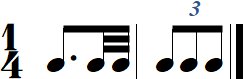
\includegraphics[scale=0.20]{pictures/score5.png}
and 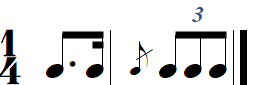
\includegraphics[scale=0.20]{pictures/score4.png}.  Wheighted
parsing associates a cost to each solution, and our framework
aims at selecting the best one with respect to this cost.
\endex
\end{example}



%%%%%%%%%%%%%%%%%%%%%%%%%%%%%%%%%%%%%%%%%%%%%%%%%%%%%%%%%%%%%%%%%%%%%%%%%%%%%%%%%%%%%%%%%%%%%%%%%%%%
%% prelin
%%%%%%%%%%%%%%%%%%%%%%%%%%%%%%%%%%%%%%%%%%%%%%%%%%%%%%%%%%%%%%%%%%%%%%%%%%%%%%%%%%%%%%%%%%%%%%%%%%%%

\section{Preliminary Notions}
\label{section:prelim}\label{sec:prelim}

%notations: for set $S$ : sets of sequences $S^*$ and $S^+$...
%interval $[i..j]$ of natural numbers

%\paragraph*{Semirings}
\label{section:semiring}\label{sec:semiring}
% !TEX root = main.tex
%
% Semiring basics
%
We shall consider semirings for the weight values of our language models.
\florent{The results are established for a general class of semirings. They can be instantiated for concrete cases}
%
\philippe{There is sometimes a confusion in the text between the struture and the domain $\Semiring$. Not
essential}.
A \emph{semiring} $\< \Semiring, \oplus, \zero, \otimes, \one>$ 
is a structure with a domain~$\Semiring$,
equipped with two associative
binary operators~$\oplus$ and $\otimes$,
with respective neutral elements $\zero$ and $\one$, and such that:
%$\< \mathbb{S}, \oplus, \zero>$ is a commutative monoid
%$\< \mathbb{S}, \otimes, \one>$ is a monoid
\begin{itemize}
\item $\oplus$ is commutative: 
 $\< \Semiring, \oplus, \zero>$ is a commutative monoid 
   and $\< \Semiring, \otimes, \one>$ a monoid,
\item $\otimes$ distributes over~$\oplus$:  $\forall x, y, z \in \mathbb{S}$,
$x \otimes (y \oplus z) = (x \otimes y) \oplus (x \otimes z)$, 
and $(x \oplus y) \otimes z = (x \otimes z) \oplus (y \otimes z)$,
\item $\zero$ is absorbing for~$\otimes$: 
$\forall x\in \mathbb{S}$, $\zero \otimes x = x \otimes \zero = \zero$.
\end{itemize}
%Components of a semiring~$\Semiring$ may be subscripted by~$\Semiring$ when needed.
%We simply write $x \in \Semiring$ to mean $x \in \mathbb{S}$.
%
Intuitively, in the models presented in this paper, 
$\oplus$ selects an optimal value from two given values, 
in order to handle non-determinism, 
and $\otimes$ combines two values into a single value, 
in a chaining of transitions.
%and let $\< \Semiring, \oplus, \zero, \otimes, \one>$ be a {semiring}, 

\medskip%\noindent
A semiring $\Semiring$ is \emph{commutative} if $\otimes$ is commutative.
It is \emph{idempotent} if for all $x \in \Semiring$, $x \oplus x = x$.
%
Every idempotent semiring~$\Semiring$ induces 
a partial ordering~$\leq_\oplus$ 
called the \emph{natural ordering} of~$\Semiring$~\cite{Mohri02semiring} 
defined,  by: 
%implicitly defined by the semiring $\Semiring$ 
for all $x, y\in \Semiring$,
$x \leq_\oplus y \;\mbox{iff}\; x \oplus y = x$.
%(see~\cite{Mohri02semiring} for the proof that it is an ordering).
%
The natural ordering is sometimes defined in the opposite direction~\cite{DrosteKuich09semirings};
We follow here the direction  %follows \cite{Mohri02semiring}, and 
that coincides with the usual ordering on the Tropical semiring \emph{min-plus} 
(Figure~\ref{fig:semirings}).
%
\noindent
An idempotent semiring $\Semiring$~is called \emph{total} if
it~$\leq_\oplus$ is total
\ie when for all $x, y \in \Semiring$, either $x \oplus y = x$ or $x \oplus y = y$.
\florent{is total necessary?}

\begin{lemma}[Monotony, \cite{Mohri02semiring}] \label{lem:monotonic}
Let $\< \Semiring, \oplus, \zero, \otimes, \one>$ be an idempotent semiring.
For all $x, y, z  \in \Semiring$,  
if $x \leq_\oplus y$ then
$x \oplus z \leq_\oplus y \oplus z$,
$x \otimes z \leq_\oplus y \otimes z$
and $z \otimes x \leq_\oplus z \otimes y$.
\end{lemma}   
%When  holds, 
%We say in this case that 
To express the property of Lemma~\ref{lem:monotonic}, we call
$\Semiring$ \emph{monotonic} \wrt $\leq_\oplus$.
%A semiring $\Semiring$ 
%is \emph{monotonic} \wrt a partial ordering~$\leq$ 
%iff for all $x, y, z  \in \Semiring$,  $x \leq y$ implies
%$x \oplus z \leq y \oplus z$,
%$x \otimes z \leq y \otimes z$,
%and $z \otimes x \leq z \otimes y$.
%
Another important semiring property in the context of optimization
is {superiority}~\cite{Huang08advanceddynamic}, 
which corresponds to the 
\emph{non-negative weights} condition in shortest-path algorithms~\cite{Dijkstra59anote}.
Intuitively, it means that combining elements with $\otimes$ always increase their weight. 
Formally, it is defined as the property ($i$) below. %of the following lemma.

\begin{lemma}[Superiority, Boundedness]
\label{lem:superior}\label{lem:bounded}
Let $\< \Semiring, \oplus, \zero, \otimes, \one>$ be an idempotent semiring.
The two following statements are equivalent:
\begin{itemize}
\item [$i.$] for all $x, y \in \Semiring$,  
$x \leq_\oplus x \otimes y$ and 
$y \leq_\oplus x \otimes y$
\item[$ii.$] for all $x \in \Semiring$,  $\one \oplus x = \one$.
\end{itemize}
\end{lemma}
%
\begin{proof} %(Lemma~\ref{lem:bounded})
$(ii) \Rightarrow (i)$ : 
$x \oplus (x \otimes y) = x \otimes (\one \oplus y) = x$, 
by distributivity of~$\otimes$ over~$\oplus$. 
Hence $x \leq_\oplus x \otimes y$.
Similarly, $y \oplus (x \otimes y) = (\one \oplus x) \otimes y = y$, 
hence $y \leq_\oplus x \otimes y$.
%
$(i) \Rightarrow (ii)$ :
%$(i)$ implies that $\one \leq_\oplus x$ for all $x \in \Semiring$, 
by the second inequality of ($i$), with $y = \one$, 
$\one \leq_\oplus x \otimes \one = x$, \ie, 
by definition of $\leq_\oplus$, $\one \oplus x = \one$.
%\qed
\end{proof}

In~\cite{Huang08advanceddynamic}, when the property~$(i)$ holds,  
$\Semiring$ is called \emph{superior} \wrt the ordering~$\leq_\oplus$.
We have seen in the proof of Lemma~\ref{lem:bounded} that it implies that 
$\one \leq_\oplus x$ for all $x \in \Semiring$.
Similarly, by the first inequality of ($i$) with $y = \zero$,  
$x \leq_\oplus x \otimes \zero = \zero$.
%
Hence, in a superior semiring, % \wrt~$\leq$, 
it holds that %$\one \leq \zero$
for all $x \in \Semiring$, $\one \leq_\oplus x \leq_\oplus \zero$.
%
Intuitively, from an optimization point of view,
it means that $\one$ is the best value, and $\zero$ the worst.
%** superior implies $\Semiring$ bounded~\cite{Mohri02semiring} see **
%
In~\cite{Mohri02semiring}, 
$\Semiring$ with the property ($ii$) of Lemma~\ref{lem:bounded}  
is called \emph{bounded} -- we shall use this term in the rest of the paper. 
% \emph{negative boundedness} 
It implies that, when looking for a best path in a graph whose edges
are weighted by values of $\Semiring$, the loops can be safely avoided,
because, for all $x \in \Semiring$ and $n \geq 1$, 
 $x \oplus x^n = x \otimes (\one \oplus x^{n-1}) = x$.


\begin{lemma}
Every bounded semiring is idempotent.
\end{lemma}
\begin{proof}
By boundedness, $\one \oplus \one = \one$, 
and idempotency follows by multiplying
both sides by $x$ and distributing. 
%\qed
\end{proof}

%\medskip
\noindent
\philippe{Here the difference between $\Semiring$ as a structure and as a domain is blurred.}
We shall need below infinite sums with~$\oplus$.
A semiring~$\Semiring$ is called \emph{complete}~\cite{Droste09handbook} 
%(\cite{Droste09handbook} chapter 1) %\cite{Kuich97semirings}
if it has an %infinite sum 
operation $\bigoplus_{i \in I} x_i$
for every family
$(x_i)_{i \in I}$ %$\{ x_i \mid i \in I \}$
of elements of $\dom(\Semiring)$ over an index set $I \subset \mathbb{N}$, such that:
\philippe{$j\in \mathbb{N}$: $j$ is en element of $\mathbb{N}$, not the same s $j\subset \mathbb{N}$}
%the following holds: %properties
\begin{description}
\item[$i.$]
\emph{infinite sums extend finite sums:}\\
$\displaystyle\bigoplus_{i \in \emptyset} x_i = \zero$,\quad 
      $\forall j\in \mathbb{N}, \displaystyle\bigoplus_{i \in \{ j \}} x_i = x_j$,
      $\forall j, k\in \mathbb{N}, j\neq k, 
      \displaystyle\bigoplus_{i \in \{ j, k \}} x_i = x_j \oplus x_k$,
%
\item[$ii.$]
\emph{associativity and commutativity:}\\
for all $I \subseteq \mathbb{N}$
and all partition $(I_{j})_{j \in J}$ of $I$, %\subseteq \mathbb{N}$, 
\(
\displaystyle
\bigoplus_{j \in J}\bigoplus_{i \in I_j} x_i = 
\bigoplus_{i \in I} x_i
\),
%
\item[$iii.$] 
\emph{distributivity of product over infinite sum:}\\
for all $I \subseteq \mathbb{N}$,
\(
\displaystyle
\bigoplus_{i \in I} (x \otimes y_i) = x \otimes \bigoplus_{i\in I} y_i\), and
\(
\displaystyle
\bigoplus_{i \in I} (x_i \otimes y) = (\bigoplus_{i \in I} x_i ) \otimes y\).
\end{description}



%\begin{example}
%Figure~\ref{fig:semirings} presents examples of semirings interesting in practice 
%and enjoying the above properties.
%\end{example}


\begin{figure}[t]
\begin{center}
\begin{tabular}{|c|c|C{2em}|C{2em}|C{2em}|C{2em}|}
\hline
        & domain & $\oplus$ & $\otimes$ & $\zero$  & $\one$\\ %& nat. ordering\\
\hline\hline
Boolean & $\{\bot, \top\}$ & $\vee$ & $\wedge$ & $\bot$ & $\top$\\ %& $\top \leq_\oplus \bot$  \\
\hline
Counting & $\mathbb{N}$ & $+$ & $\times$ & 0 & 1 \\
\hline
Viterbi & $[0, 1] \subset \mathbb{R}$ & $\mathit{max}$ & $\times$ & 0 & 1\\ % & $x \leq_\oplus y \iff x \ge y$  \\
\hline
Tropical min-plus & $\mathbb{R}_+ \cup \{ \infty\}$ & $\mathit{min}$ & $+$ & $\infty$ & $0$\\ % & $x \leq_\oplus y \iff x \leq y$   \\
\hline
%MaxPlus & $\mathbb{Q} \cup \{ -\infty\}$ & $\mathsf{max}$ & $+$ & $-\infty$ & $0$ \\
%\hline
%Word lang. & $2^{\Sigma^*}$ & $\cup$ & $\cdot$ & $\emptyset$ & $\{ \varepsilon \}$ \\
%\hline
\end{tabular}
\end{center}
\vskip-1em
\caption{Some commutative, bounded, total and complete semirings.}
\label{fig:semirings}
\end{figure}
\florent{results of this paper: for semirings commutative, bounded, total and complete}

%%% semiring properties used in paper
% - commutative
% - bounded (implies idempotent and superior)
% - total
% - complete






%\paragraph*{Label Theory}
\label{section:symbols}
% !TEX root = main.tex
%
% Label Theory
%
\subsection{Label Theories} 
%\noindent
We define the functions labeling the transitions of SW automata and transducers,
generalizing the Boolean algebras of~\cite{dAntoniVeanes17CAV}.
%from Boolean to other semiring domains.
%
We consider \emph{alphabets}, which are non-empty countable 
%\reviews{1) non-empty}
sets of symbols
denoted by $\Sigma$, $\Delta$,...
Moreover, $\Sigma^*$ is the set of finite sequences (\emph{words}) over
$\Sigma$, $\varepsilon$ the empty word, $\Sigma^+ = \Sigma^* \setminus \{ \varepsilon \}$,
and $u v$ denotes the concatenation of $u, v \in \Sigma^*$.
%where $au$, and $bv$, denote the concatenation
%of the symbol $a \in \Sigma$ (resp. $b \in \Delta$)
%with a word $u \in \Sigma^*$ (resp. $v \in \Delta^*$).
%\lydia{added $u$ and $v$ def}

Given a semiring $\< \Semiring, \oplus, \zero, \otimes, \one>$,
a \emph{label theory} $\bar\Phi$ over~$\Semiring$
is an indexed family of recursively enumerable sets denoted by
%\reviews{1) $\bar\Phi$ is a $(\Sigma \cup \Sigma \times \Delta)$-indexed family...}
%$\Phi_\epsilon \subseteq \Semiring$, % containing constant functions valued in $\Semiring$,
$\Phi_\Sigma$, %and $\Phi_\Delta$,
containing unary functions of type $\Sigma \to \Semiring$, %resp. $\Delta \to \Semiring$,
or $\Phi_{\Sigma, \Delta}$, containing binary functions $\Sigma \times \Delta \to \Semiring$,
and such that:
%\florent{unary for \SWA (weight depends on input symbol) and binary for transducers and VPA (weight depends on input symbol AND output or stack symbol)}
\begin{itemize}
\item %\noindent --
     for all $\Phi_{\Sigma, \Delta} \in \bar\Phi$, we have
     $\Phi_{\Sigma} \in \bar\Phi$ and $\Phi_{\Delta} \in \bar\Phi$
%
%\item %\noindent --
%every $\Phi_{\Sigma}\in \bar\Phi$ contains all the constant functions from $\Sigma$ into $\Semiring$,
%\reviews{3) contradicts $\Sigma$ countable}
%\reviews{1) $\forall \Sigma$...}
%
\item %\noindent --
      for all $\Phi_{\Sigma} \in \bar\Phi$, 
      for all $\phi \in \Phi_\Sigma$, and $\alpha \in \Semiring$ 
      $\alpha \otimes \phi : x \mapsto \alpha \otimes \phi(x)$,
      and $\phi \otimes \alpha : x \mapsto \phi(x) \otimes \alpha$  %\phantom{--} 
      belong to $\Phi_\Sigma$, and similarly for $\oplus$
      and for $\Phi_{\Sigma, \Delta}$
%
\item %\noindent --
      for all $\Phi_{\Sigma} \in \bar\Phi$, 
      for all $\phi, \phi' \in \Phi_\Sigma$,
      $\phi \otimes \phi': x \mapsto \phi(x) \otimes \phi'(x)$ belongs to $\Phi_\Sigma$
%
\item %\noindent --
	  for all $\Phi_{\Sigma, \Delta} \in \bar\Phi$,
      for all $\eta, \eta' \in \Phi_{\Sigma, \Delta}$
      $\eta \otimes \eta': x, y \mapsto \eta(x, y) \otimes \eta'(x, y)$ belongs to $\Phi_{\Sigma, \Delta}$
%
\item %\noindent --
      for all $\Phi_{\Sigma}, \Phi_{\Sigma, \Delta} \in \bar\Phi$,
      for all $\phi \in \Phi_\Sigma$ and $\eta \in \Phi_{\Sigma, \Delta}$,
      $\phi \otimes_1 \eta: x, y \mapsto \phi(x) \otimes \eta(x, y)$ and
      $\eta \otimes_1 \phi: x, y \mapsto \eta(x, y) \otimes \phi(x)$
      belong to $\Phi_{\Sigma, \Delta}$
%
\item %\noindent --
      for all $\Phi_{\Delta}, \Phi_{\Sigma, \Delta} \in \bar\Phi$,
      for all $\psi \in \Phi_\Delta$ and $\eta \in \Phi_{\Sigma, \Delta}$,
      $\psi \otimes_2 \eta: x, y \mapsto \psi(y) \otimes \eta(x, y)$ and
      $\eta \otimes_2 \psi: x, y \mapsto \eta(x, y) \otimes \psi(y)$
      belong to $\Phi_{\Sigma, \Delta}$
%
\item %\noindent --
      similar closures hold for $\oplus$.
\end{itemize}

%\noindent --
%the partial applications $\eta \in \Phi_{\Sigma, \Delta}$
%and $\eta_a: y \mapsto \eta(a, y)$ for $a \in \Sigma$ %and $y \in \Delta$
%and\\
%\phantom{--} $\eta_b: x \mapsto \eta(x, b)$ for $b \in \Delta$ %and $x \in \Sigma$,
%belong respectively to~$\Phi_\Delta$ and~$\Phi_\Sigma$.
\florent{partial application is needed?}

%Moreover, these sets are required to be closed under the
%operators~$\oplus$ and~$\otimes$ of~$\Semiring$:
%for all $\phi, \phi' \in \Phi_\Sigma$,
%$\psi, \psi' \in \Phi_\Delta$,
%and $\eta, \eta' \in \Phi_{\Sigma, \Delta}$, %the function
%%
%\begin{center}
%\begin{tabular}{cclll}
%$\phi \otimes \phi'$ & : & $x \mapsto \phi(x) \otimes \phi'(x)$ & belongs to $\Phi_\Sigma$,\\
%$\psi \otimes \psi'$ & : & $y \mapsto \psi(y) \otimes \psi'(y)$ & belongs to $\Phi_\Delta$,\\
%$\phi \otimes \eta$\;  & : & $x, y \mapsto \phi(x) \otimes \eta(x, y)$ & belongs to $\Phi_{\Sigma, \Delta}$,\\
%$\eta \otimes \psi$  & : & $x, y \mapsto \eta(x, y) \otimes \psi(y)$ & belongs to $\Phi_{\Sigma, \Delta}$,\\
%$\eta \otimes \eta'$ & : & $x, y \mapsto \eta(x, y) \otimes \eta'(x, y)$ & belongs to $\Phi_{\Sigma, \Delta}$, &
%\multicolumn{1}{r}{and similarly for $\oplus$.}\\ %the same also holds for the binary sum operator $\oplus$.
%\end{tabular}
%\end{center}
%
%Finally, it is also required
%% that the codomain of every function of $\Phi_\Sigma$ and $\Phi_\Delta$
%% is a subset of $\Phi_\epsilon$, and
%that the partial applications of a function $\eta \in \Phi_{\Sigma, \Delta}$,
%resp.  $\eta_a: y \mapsto f(a, y)$ for $a \in \Sigma$ and $y \in \Delta$
%and  $\eta_b: x \mapsto f(x, b)$ for $b \in \Delta$ and $x \in \Sigma$,
%belong resp. to~$\Phi_\Sigma$ and~$\Phi_\Delta$.
%
\noindent
When the semiring $\Semiring$ is complete, we consider moreover 
the following operators on the functions of~$\bar\Phi$. % a label theory.
%(we use overloading to simplify notations):
\[
\begin{array}{ll}
\bigoplus_\Sigma : \Phi_\Sigma \to \Semiring,\
  \phi \mapsto \displaystyle\bigoplus_{a \in \Sigma} \phi(a)\\
%  
\bigoplus^1_\Sigma :
  \Phi_{\Sigma,\Delta} \to \Phi_\Delta,\
  \eta \mapsto \bigl( y \mapsto \displaystyle\bigoplus_{a \in \Sigma} \eta(a, y) \bigr) &
%
\bigoplus^2_\Delta :
  \Phi_{\Sigma,\Delta} \to \Phi_\Sigma,\
  \eta \mapsto \bigl( x \mapsto \displaystyle\bigoplus_{b \in \Delta} \eta(x, b) \bigr)\\
\end{array}
\]
Intuitively, $\bigoplus_\Sigma$
returns the global minimum, \wrt $\leq_\oplus$, of a function $\phi$ of~$\Phi_\Sigma$,
and $\bigoplus^1_\Sigma$, $\bigoplus^2_\Delta$ return partial minimums of 
a function $\phi$ of~$\Phi_{\Sigma,\Delta}$.

%\medskip\noindent
%In what follows, we might omit the sub- and superscripts in
%\philippe{On peut simplifier la notation et supprimer cette discussion?}
%$\otimes_1$, $\bigoplus^1_\Sigma$...,
%%$\otimes_2$, $\oplus_1$, $\oplus_2$
%when there is no ambiguity.
%We shall keep them only for the special case $\Sigma = \Delta$,
%\ie $\eta \in \Phi_{\Sigma, \Sigma}$, % for~$\otimes_1$ above,
%%and $\eta \in \Phi_{\Delta, \Delta}$ for~$\otimes_2$.
%%Similarly as for the above product and sum of functions,
%%the superscripts in $\bigoplus^1_\Sigma$ and $\bigoplus^2_\Sigma$
%%shall be reserved to the ambiguous case of $\Phi_{\Sigma,\Sigma}$,
%in order to be able to distinguish between the first and the second argument.
%
%\begin{definition}\label{def:label-th-complete}
%A label theory~$\bar\Phi$ is \emph{complete} when

\noindent
We assume that when the underlying semiring~$\Semiring$ is complete:
\begin{itemize}
\item 
	  for all $\Phi_{\Sigma, \Delta} \in \bar\Phi$
	  and all $\eta \in \Phi_{\Sigma, \Delta}$,
	  $\bigoplus^1_\Sigma \eta \in \Phi_{\Delta}$ and
	  $\bigoplus^2_\Delta \eta \in \Phi_{\Sigma}$.
\end{itemize}


\begin{example}\label{distance-time}
We return to Example~\ref{ex:running}.
Let $\Deltai$ be the subset of $\Delta$ without markup symbols.
In order to align the input in $\Sigma^*$ %sequence
with a music score, % in $\Delta^*$, 
we must account for
the expressive timing of human performance that
results in small time shifts between an input event of~$\Sigma$ and the corresponding
notation event in~$\Deltai$.
These shifts can be weighted as the time distance between both,
computed in the tropical semiring by $\delta \in \Phi_{\Sigma, \Deltai}$,
defined as follows:
\[
%\mbox{for~all}\,
%\mu\ts{\tau} \in \Sigma,
%\nu\ts{\tau'} \in \Deltai,
\delta(\mu\ts{\tau}, \nu\ts{\tau'}) =
\left\{
\begin{array}{ll}
   | \tau' - \tau | & \mathrm{if}\  \nu \rm{\ corresponds\ to\ } \mu,\\
   \zero  & \mathrm{otherwise}
\end{array}
\right.
\]
%The performance is
%$I = [ \mu_1\ts{0.07}, \mu_2, 0.72>, \<\mu_3, 0.91>, \<\mu_4, 1.05>, \<\mu_5, 1.36>, \<\mu_6, 1.71>]$,
%and the (linearized) score is
%$[\<\nu_1,0>, \<\nu_2,\frac{3}{4}>, \<\nu_3,\frac{7}{8}>, \<\nu_4,1>, \<\nu_5,\frac{4}{3}>, \<\nu_6\frac{5}{3}>]$
%Assuming the pairwise correspondence of MIDI symbols
%$\mu_i$ and notation symbols $\nu_i$, for $i \in [1, 6]$,
\florent{$I$ et $O$ deja donnés dans ex.\ref{ex:running}}
The distance between $I$ and $O$ is the  aggregation with $\otimes$
of the pairwise differences between the
timestamps. In the tropical semiring, this yields
$|0.07 - 0| + |0.72 - \frac{3}{4}| + |0.91- \frac{7}{8} | +
|1.05-1| + |1.36-\frac{4}{3}| + |1.71-\frac{5}{3}|= 0.255$.
\endex
\end{example}


% !TEX root = main.tex
%
% Properties of Label Theory

The following facts are immediate consequences of the definitions of 
the operators on the functions of labels theories. % in Section~\ref{sec:prelim}.

\begin{lemma} \label{lem:label-th}
For a complete label theory $\bar\Phi$, 
for all $\Phi_{\Sigma}, \Phi_{\Delta}, \Phi_{\Sigma, \Delta} \in \bar\Phi$, 
$\alpha \in \Semiring$,
$\phi, \phi' \in \Phi_{\Sigma}$,
$\psi \in \Phi_{\Delta}$, and
$\eta \in \Phi_{\Sigma, \Delta}$,
it holds that:
%
\begin{enumerate}
\item[$i.$]
\( \bigoplus_{\Sigma}\bigoplus^2_{\Delta} \eta = \bigoplus_{\Delta}\bigoplus^1_{\Sigma} \eta \).
\item[$ii.$]
\( \alpha \otimes \bigoplus_{\Sigma} \phi = \bigoplus_{\Sigma} (\alpha \otimes \phi) \) and
\( \bigl( \bigoplus_{\Sigma} \phi \bigr) \otimes\alpha = \bigoplus_{\Sigma} (\phi \otimes \alpha) \),
and similarly for~$\oplus$.
\item[$iii.$]
\( \bigl(\bigoplus_{\Sigma} \phi\bigr) \oplus \bigl(\bigoplus_{\Sigma} \phi'\bigr)
   = \bigoplus_{\Sigma} (\phi \oplus \phi') \) and
\( \bigl(\bigoplus_{\Sigma} \phi\bigr) \otimes \bigl(\bigoplus_{\Sigma} \phi'\bigr)
   = \bigoplus_{\Sigma} (\phi \otimes \phi') \).
\item[$iv.$]
\( \bigl(\bigoplus^2_{\Delta} \eta\bigr) \oplus \bigl(\bigoplus^2_{\Delta} \eta' \bigr) =
 \bigoplus^2_{\Delta} (\eta \oplus \eta') \), and
\( \bigl(\bigoplus^2_{\Delta} \eta\bigr) \otimes \bigl(\bigoplus^2_{\Delta} \eta' \bigr) =
 \bigoplus^2_{\Delta} (\eta \otimes \eta') \).
\item[$v.$]
%\( \phi \oplus \bigl(\bigoplus_{\Delta} \eta\bigr) = \bigoplus_{\Delta} (\phi \oplus \eta) \),
\( \phi \otimes \bigl(\bigoplus^2_{\Delta} \eta\bigr) = \bigoplus_{\Delta} (\phi \otimes_1 \eta) \), and
\( \bigl(\bigoplus^2_{\Delta} \eta\bigr) \otimes \phi = \bigoplus_{\Delta} (\eta \otimes_1 \phi) \),\\
and similarly for~$\oplus$.
\item[$vi.$]
%\( \psi \oplus \bigl(\bigoplus_{\Sigma} \eta\bigr) = \bigoplus_{\Sigma} (\psi \oplus \eta) \),
\( \psi \otimes \bigl(\bigoplus^1_{\Sigma} \eta\bigr) = \bigoplus_{\Sigma} (\psi \otimes_2 \eta) \), and
\( \bigl(\bigoplus^1_{\Sigma} \eta\bigr) \otimes \psi = \bigoplus_{\Sigma} (\eta \otimes_2 \psi) \),\\
and similarly for~$\oplus$.
\end{enumerate}
\end{lemma}




\noindent 
The following property of label theories will be useful in 
the following results, in order to ensure 
the computability of the above infinite sum operators.
%
\begin{definition}\label{def:effective}
A label theory $\bar\Phi$ is called \emph{effective} when
for all $\Phi_{\Sigma}, \Phi_{\Sigma, \Delta} \in \bar\Phi$, 
$\phi \in \Phi_\Sigma$ and $\eta \in \Phi_{\Sigma, \Delta}$,
$\bigoplus_{\Sigma} \phi$,
$\bigoplus_{\Delta}\bigoplus^1_{\Sigma} \eta$, and
$\bigoplus_{\Sigma}\bigoplus^2_{\Delta} \eta$
can be effectively computed from $\phi$ and $\eta$,
as well as one symbol, at least, 
reaching each of these bounds.
%the number of symbols reaching these bounds is finite
\end{definition}

The effectiveness is a strong restriction on label theories.
It is however not unrealistic in the context of the problems for languages models considered below, 
namely the combination of automata, best-search and symbolic weighted parsing.
%
In fact, every instance of such problems comes with a finite number of automata, each one containing a finite number of functions in a label theory, in their transitions. 
We may assume that the global minimums $\bigoplus_{\Sigma} \phi$,
$\bigoplus_{\Delta}\bigoplus^1_{\Sigma} \eta$, and
$\bigoplus_{\Sigma}\bigoplus^2_{\Delta} \eta$
of all these functions are known.
%
Then, the other functions considered when solving the problems are obtained by combination with the above operators.  
These operators preserve effectiveness, as long as the semiring is monotonic. 
In practice, the combinations may be represented by structures like 
Algebraic Decision Diagrams~\cite{Bahar97ADD}.

%we call \emph{summary} of a function
%$\phi \in \Phi_\Sigma$,
%resp. $\eta \in \Phi_{\Sigma, \Delta}$,
%the value $\bigoplus_{a \in \Sigma} \phi(a)$,
%resp. $\bigoplus_{a \in \Sigma} \bigoplus_{b \in \Delta} \eta(a, b)$.
%By definition of infinite sums in complete semirings,
%a summary of $\phi \oplus \phi'$, $\alpha \otimes \phi$ and $\phi \otimes \alpha$
%can be computed from $\alpha \in \Semiring$ and summaries of $\phi$ and $\phi'$ in $\Phi_{\Sigma}$,
%using the operators of $\Semiring$,
%and the same holds for $\Phi_{\Delta}$ and $\Phi_{\Sigma, \Delta}$.


%there is an oracle returning, in constant time,
%$\bigoplus_{\Sigma} \phi$,
%$\bigoplus_{\Sigma} \eta$, and
%$\bigoplus_{\Delta} \eta$
%and one symbol where the function reaches this minimum,
%denoted $\bigominus_\Sigma \phi$

%\begin{definition}\label{def:label-th-convex}
%Let $\Omega$ be an alphabet
%A function $\phi \in \Phi_\Sigma$ in a label theory over a complete semiring $\Semiring$
%is called $k$-\emph{convex}, for a natural number $k$, iff
%$\mathrm{card}\{ a \in \Sigma \mid \phi(a) = \bigoplus_{\Sigma} \phi \} \leq k$.
%\end{definition}
%A label theory is $k$-convex if all its functions are $k$-convex.

%s.t. for all $\phi \in \Phii$,
%$\psi \in \Phir$,
%and $\eta \in \Phicr$,
%$\displaystyle\bigoplus_{a \in \Omegai} \phi(a)$
%$\displaystyle\bigoplus_{r \in \Omegar} \phi(r)$ and
%$\displaystyle\bigoplus_{{\call{c}} \in \Omegac}
%\displaystyle\bigoplus_{{\return{r}} \in \Omegar} \eta({\call{c}}, {\return{r}})$
%are computable...
%
% total ?
% monotonic and superior writ natural ordering
%Regarding the infinite sum operator, note that
%$\bigoplus_{x \in \Phi_\Omega} \phi(x)$,
%$\bigoplus_{y \in \Phi_\Delta} \psi(y)$, and
%... exist and in $\Semiring$.



%Concretely, in one of the language models defined below,
%we consider a finite number of base functions $\phi, \eta$ of the underlying label theory,
%labelling transitions, and combine them with the above operators for construction of
%other models.
%The combinations might be represented by dags (diagrams) whose leaves are labeled
%by base functions and inner nodes by operators.
% we can compute the value of a diagram in time...




%%%%%%%%%%%%%%%%%%%%%%%%%%%%%%%%%%%%%%%%%%%%%%%%%%%%%%%%%%%%%%%%%%%%%%%%%%%%%%%%%%%%%%%%%%%%%%%%%%%%
%% SWT & SWA
%%%%%%%%%%%%%%%%%%%%%%%%%%%%%%%%%%%%%%%%%%%%%%%%%%%%%%%%%%%%%%%%%%%%%%%%%%%%%%%%%%%%%%%%%%%%%%%%%%%%

\section{SW Automata and Transducers}
\label{section:transducer}\label{sec:transducer}
\label{section:SWA}\label{sec:SWA}
\label{section:SWT}\label{sec:SWT}

We follow the approach of~\cite{Mohri03ijfcs} for the computation of distances
between words and languages
and extend it to infinite alphabets.
% with models of symbolic weighted automata and transducers.
%
The models presented in this section generalize weighted automata and transducers~\cite{Droste09handbook}
%over finite alphabets, see \eg~\cite{Mohri03ijfcs},
by labeling each transition with a weight function
that takes the input and output symbols as parameters.
These functions generalize the guards 
of symbolic automata~\cite{Veanes12symbolic,dAntoniVeanes17CAV,dAntoni21CACM},
from Boolean domains to commutative semirings.
%
They are particular cases of the very general model of 
Weighted Symbolic Automata with Data Storage~\cite{Herrmann16dlt}. 

%\subsection{Definitions} \label{sec:SWTdef}\label{sec:SWAdef}
%(SWT)
\noindent
Let $\Semiring$ be a commutative semiring,
$\Sigma$ and $\Delta$ be alphabets called \emph{input} and \emph{output} respectively, %{alphabets},
and $\bar\Phi$ be a label theory over $\Semiring$
containing $\Phi_\Sigma$, $\Phi_\Delta$, $\Phi_{\Sigma, \Delta}$.

\begin{definition}
\label{def:transducer} \label{def:SWT}
A \emph{symbolic-weighted transducer} (\SWT)
over $\Sigma$, $\Delta$, $\Semiring$ and $\bar\Phi$
%the input and output alphabets~$\Sigma$ and $\Delta$ with label theory $\bar\Phi$, and the semiring $\Semiring$
is a tuple
$T = \< Q, \init, \bar{\wei}, \final >$,
where $Q$ is a finite set of states,
$\mathsf{in} \colon Q \to \Semiring$   %\Phi_{\Sigma, \Delta}
(respectively $\mathsf{out} \colon Q \to \Semiring$)  %\Phi_{\Sigma, \Delta}
are functions defining the weight for entering
(respectively leaving) computation in a state,
and $\bar{\wei}$ is a triplet of transition functions
$\wei_{10}: Q \times Q \to \Phi_{\Sigma}$,
$\wei_{01}: Q \times Q \to \Phi_{\Delta}$, and
$\wei_{11}: Q \times Q \to \Phi_{\Sigma, \Delta}$.
\end{definition}
%
\noindent
%We call the \emph{number of transitions} of $T$ the number of pairs of states
%$q, q' \in Q$ such that $\wei_{10}$ or $\wei_{01}$ or $\wei_{11}$
%is not the constant $\zero$.
%
\noindent
A tuple of $Q \times (\Sigma \cup \{ \varepsilon \}) \times (\Delta \cup \{ \varepsilon \}) \times Q \to \Semiring$
is called a \emph{transition} of $T$.
For convenience, we shall sometimes present the above $\wei_{10}$, $\wei_{01}$, $\wei_{11}$
%(overloading the function names),
as mappings associating to every transition a weight value in $\Semiring$ as follows,
for every $q, q' \in Q$, $a \in \Sigma$,  $b \in \Delta$:
\[
\begin{array}{rcll}
\wei_{10}(q, a, \varepsilon, q') & = & \phi(a) & %\wei_\Sigma(q, q')(a)
\quad\mathrm{where~} \phi = \wei_{10}(q, q') \in \Phi_\Sigma,\\
\wei_{01}(q, \varepsilon, b, q') & = & \psi(b) &
\quad\mathrm{where~} \psi = \wei_{01}(q, q') \in \Phi_\Delta,\\
\wei_{11}(q, a, b, q') & = & \eta(a, b) &
\quad\mathrm{where~} \eta = \wei_{11}(q, q') \in \Phi_{\Sigma, \Delta}.\\
\end{array}
\]
%
\noindent
% The symbolic-weighted transducer
The \SWT $T$ computes on pairs $\< s, t> \in \Sigma^* \times \Delta^*$,
$s$ and $t$, being respectively called \emph{input} and \emph{output} word.
\florent{It compute asynchronously: advance in $s$ and not in $t$ ($\wei_{10}$),
or the opposite ($\wei_{01}$),
or advance in both $s$ and $t$ ($\wei_{11}$).}
% \noindent
The semantics of $T$ is
based on an intermediate function $\weight_T$
defined recursively as follows, for every states $q, q' \in Q$,
and every pairs of strings $\< s, t> \in \Sigma^* \times \Delta^*$.
% \setminus \{ \< \varepsilon, \varepsilon >\}$,
%
%$a \in \Sigma$, $u \in \Sigma^*$, $b\in \Delta$, $v\in \Delta^*$, by:
%
\begin{align}
%\weight_T(q, \varepsilon, \varepsilon, q)  & = \one \label{eq:SWT-weight}\\ %\final(q)\\
%\weight_T(q, \varepsilon, \varepsilon, q') & = \zero \quad \mathrm{if~} q \neq q'\nonumber\\
\weight_T(q, \varepsilon, \varepsilon, q')  & = \one
 \quad \mathrm{if~} q = q' \mathrm{~and~} \zero \mathrm{~otherwise} \label{eq:SWT-weight}\\
\weight_T(q, s, t, q') & = \displaystyle\bigoplus_{\begin{array}{c}
                                                   \scriptstyle q'' \in Q\\[-1ex]
                                                   \scriptstyle s = ua,\, a \in \Sigma
                                                   \end{array}}
    \weight_T(q, u, t, q'') \otimes \wei_{10}(q'', a, \varepsilon, q')\nonumber\\
                    & \oplus \displaystyle\bigoplus_{\begin{array}{c}
                                                     \scriptstyle q'' \in Q\\[-1ex]
                                                     \scriptstyle t = vb,\, b \in \Delta\\
                                                     \end{array}}
    \weight_T(q, s, v, q'') \otimes \wei_{01}(q'', \varepsilon, b, q')\nonumber\\
                    & \oplus \displaystyle\bigoplus_{\begin{array}{c}
                                                     \scriptstyle q'' \in Q\\[-1ex]
                                                     \scriptstyle s = ua,\, t = vb\\
                                                     \end{array}}
    \weight_T(q, u, v, q'') \otimes \wei_{11}(q'', a, b, q')\nonumber
\end{align}


%
We recall that, by convention (Section~\ref{sec:prelim}),
an empty sum with $\bigoplus$ is equal to~$\zero$.
%
Intuitively,  a transition $\wei_{ij}(q, a, b, q')$ is interpreted as follows:
when reading $a$ and $b$ in the input and output words,
increment the current position in the input word if and only if $i = 1$,
and in the output word iff $j = 1$, %(otherwise, do not change it),
and change state from $q$ to $q'$.
When $a = \varepsilon$ (resp. $b = \varepsilon$), the current symbol
in the input (resp. output) is not read.
%
%In contrast with the models of weighted transducers over finite alphabets~\cite{Mohri03ijfcs},
%the input and output symbols at current positions are always read by transitions,
%even when they do not change the reading position the head's position.
%This is an important feature in the case of an infinite alphabet in
%order to compare input and output symbols.
%which cannot be stored in the finite memory of the transducer.
%
Since~$\zero$ is absorbing for~$\otimes$ in~$\Semiring$,
one term $\wei_{ij}(q, a, b, q'')$ equal to $\zero$ in the above expression
will be ignored in the sum, meaning that there is no possible transition
from state $q$ into state $q'$ while reading $a$ and $b$.
This is analogous to the case of a transition's guard not satisfied by $\<a, b>$ for
symbolic transducers~\cite{Veanes12transducers}.

%whereas considering the current symbol may be useful to compute a transition weight.
%(even when it does not change the head's position, like with $\varepsilon$-transitions).
%
%The cases $\weight_T(q, au, \varepsilon, q')$ and $\weight_T(q, \varepsilon, bv, q')$
%are missing in the definition of $\weight_T$.
%It means that $T$ must avoid configurations where it reached the end of
%the output word and not of the input one, or vice-versa.
%This can be done by using $\wei_{10}$ and $\wei_{01}$
%before reaching the end of word, and using a special state for this purpose.

The expression \eqref{eq:SWT-weight}
can be seen as a stateful definition of
an edit-distance between a word $s \in \Sigma^*$ and a word $t \in \Delta^*$,
see also~\cite{Mohri03ijfcs}.
Intuitively,
$\wei_{10}(q, a, \varepsilon, r)$ is the cost of
the deletion of the symbol~$a \in \Sigma$ in~$s$,
$\wei_{01}(q, \varepsilon, b, r)$ is the cost
of the insertion of~$b \in \Delta$ in $t$,
and $\wei_{11}(q, a, b, r)$ is the cost
of the substitution of  $a \in \Sigma$ by~$b \in \Delta$.
%
The cost of a sequence of such operations transforming $s$ into $t$
is the product in terms of $\otimes$ of the individual costs of the operations involved;
and the distance between $s$ and $t$ is the sum in terms of $\oplus$
of all possible products.
%
\medskip\noindent
%Let $\< s, t> \in \Sigma^* \times \Delta^*$, with $s = s_1\ldots s_n$, and $t = t_1\ldots t_m$.
Formally, the weight associated by $T$ to $\< s, t> \in \Sigma^* \times \Delta^*$ is:
%defined as follows:
\begin{equation}
T(s, t)  =
\displaystyle\bigoplus_{q, q' \in Q} \init(q)
\mathop{\otimes} \weight_T(q, s, t, q') \mathop{\otimes} \final(q')
\label{eq:SWT-value}
\end{equation}

\begin{comment}
%\begin{example}
%We can define with a \SWT the computation of a similarity measure
%between timed sequences
%similar to dynamic time warping (DTW).
%
%Let $\Semiring$  be the tropical (\emph{min-plus}) semiring of Figure~\ref{fig:semirings} and
%let $\Sigma = \Delta = \mathbb{R}_+$ be sets of timestamps.
%We consider a \SWT with one state $q$ and transitions
%$\wei_{11}(q, d, d', q) =
% \wei_{01}(q, d, d', q) =
% \wei_{10}(q, d, d', q) = |d' - d|$,
%for all $d, d' \in \mathbb{R}_+$.
%% needs reading input/output symbols even by epsilon-transitions.
%The recursive definition of $\weight_T$ correspond to the dynamic programming equations of DTW
%for the computation of an optimal match between words,
%the matching cost for two symbols being the
%the time distance between them.
%\endex
%\end{example}
\end{comment}

\begin{example}\label{ex:SWT}
We build a small \SWT over the alphabets $\Sigma$ and $\Deltai$
of Ex.~\ref{ex:running} and~\ref{distance-time},
%weighted transducer model
with two states $q_0$ and $q_1$, that
calculates the temporal distance between an input performance in~$\Sigma^*$
and the subsequence
of $\Deltai$ events in a score.
%the performance $I$ and
%the score $O$ of Example~\ref{ex:running}.
%
Given  a performed event $\mu$
and the corresponding notated event $\nu$
(\eg MIDI pitch 69 and note $\mbox{\footnotesize A4}$),
the weight  computed by the \SWT is the time distance between both,
as modeled by transitions $\wei_{11}$ below.
%
The continuation symbol $'-'$
(met for instance in \emph{ties}
$\musQuarter\!\!\!\mathrel{\raisebox{-1.5mm}{$\smile$}}\!\!\!\musEighth$,
or \emph{dots} \musQuarterDotted{})
%that represents continuation
is  skipped with no cost (transitions $\wei_{01}$).
%Likewise, the markups are ignored.
\[
\begin{array}{lclclcll}
\wei_{11}(q_0, \mu\tstamp{\tau}, \nu\tstamp{\tau'}, q_0) & = &
     \delta(\mu\tstamp{\tau}, \nu\tstamp{\tau'}) & \quad & %|\tau' - \tau| & \quad &
\wei_{11}(q_1, \mu\tstamp{\tau}, \nu\tstamp{\tau'}, q_0) & = &
     \delta(\mu\tstamp{\tau}, \nu\tstamp{\tau'}) &
     \mbox{if~} \nu \neq - \\ %|\tau' - \tau| & \quad &
\wei_{01}(q_0, \varepsilon, \mathsf{-}\tstamp{\tau'}, q_0) & = & \one & &
\wei_{01}(q_1, \varepsilon, \mathsf{-}\tstamp{\tau'}, q_0) & = & \one\\
\wei_{10}(q_0, \mu\tstamp{\tau}, \varepsilon, q_1) & = & \alpha & & %\multicolumn{3}{l}{\mathrm{for~all~} b \in \Delta}
\end{array}
\]
%
We also want to take performing errors into account,
since a performer could, for example, play an unwritten extra note.
%\lydia{reformulated this sentence}
%
%Reading such a note is modelled by
The transition $\wei_{10}$,
with a fixed weight value $\alpha \in \Semiring$,
switches from state $q_0$ (normal) to $q_1$ (error)
when reading an extra note $\mu$.
%\philippe{Comprends pas cette phrase}
%\florent{$\to$ reformulation}
The transitions in the second column below switch back to the normal state $q_0$.
% the metric computed by the \SWT is the smallest sum of point wise distances
% between dates of input and output events.
At last, we let $q_0$ be the only initial and final state, with
$\init(q_0) = \final(q_0) = \one$, and
$\init(q_1) = \final(q_1) = \zero$.
%\florent{dernière phrase utile?}
%This \SWT is capable of evaluating the differences between a score and a performance,
%all the while ensuring that performance errors are plausible.
%$\init(q_0, d, b) = \final(q_0, d, b) = \one$, and
%$\init(q_1, d, b) = \final(q_1, d, b) = \zero$,
%for all $d \in \Sigma$ and $b \in \Delta$.
\endex
\end{example}

\begin{comment}
\begin{example}
In Common Western Music Notation~\cite{Gould11Notation},
several symbols may be used to represent one single sounding event.
\lydia{unique $\to$ similar}
\florent{similar $\to$ single}
For instance, several notes can be combined with a tie,
like in $\musQuarter\!\!\!\mathrel{\raisebox{-1.5mm}{$\smile$}}\!\!\!\musEighth$,
and one note can be augmented by half its duration with a dot like in~\musQuarterDotted{}.
\lydia{modif.}
These notations are perceived equivalent when played, as their duration is equal, yet the notation is different.
We thus want to be able to compare a music score with music played by a performer.
\lydia{changed end}
%
\noindent
We propose a small weighted transducer model with two states $q_0$ and $q_1$
that calculates the distance between an input sequence of sounding
events (music "performance")
to an output sequence of written events (music "score").
% simple pointwise distance between two sequences of timestamped events **
%
Let us consider the tropical (\emph{min-plus}) semiring~$\Semiring$
of Figure~\ref{fig:semirings} and
let $\Sigma = \mathbb{R}_+$ be an input alphabet of event dates
and $\Delta = \{ \mathsf{e}, \mathsf{-} \} \times \mathbb{R}_+$
be an output alphabet of symbols with timestamps.
A symbol $\< \mathsf{e}, d > \in \Delta$ represents an event starting at date $d$,
and $\< \mathsf{-}, d >$ is a continuation of the previous event.
%More precisely, we let
%$\Sigma = \{ a, - \} \times \R_+$ and
%This example of $\Delta$ is motivated by the case of music notation,
%where several notated events (notes) can be tied together,
%with a \emph{tie} or a \emph{dot}
%meaning that they will be played as a unique sounding event.
%The timestamp of $a \in \Sigma$, denoted by $\mathsf{t}(a)$, is expressed as a rational number.

We consider a \SWT with two states $q_0$ and $q_1$ whose purpose
is to compare a recorded performance $s \in \Sigma^*$
with a notated music sheet $t \in \Delta^*$.
One timestamp $d_i \in \Sigma$ may correspond
to one notated event $\<\mathsf{e}, d'_i> \in \Delta$, in which case
the weight value computed by the \SWT is the time distance between both
(see transitions $\wei_{11}$ below).
%
If $\<\mathsf{e}, d'_i>$ is followed by continuations
$\<\mathsf{-}, d'_{i+1}>$..., they are just skipped with no cost (transitions $\wei_{01}$ or weight $\one$).
%transitions
\[
\begin{array}{rclcrcl}
\wei_{11}(q_0, d, \< \mathsf{e}, d'>, q_0) & = & |d' - d| & \quad &
\wei_{11}(q_1, d, \< \mathsf{e}, d'>, q_0) & = & |d' - d|\\
\wei_{01}(q_0, \varepsilon, \< \mathsf{-}, d'>, q_0) & = & \one & &
\wei_{01}(q_1, \varepsilon, \< \mathsf{-}, d'>, q_0) & = & \one\\
\wei_{10}(q_0, d, \varepsilon, q_1) & = & \alpha & & %\multicolumn{3}{l}{\mathrm{for~all~} b \in \Delta}
\end{array}
\]
%
We also must be able to take performing errors into account, while still being able to compare with the score,
since a performer could, for example, play an unwritten extra note.
\lydia{reformulated this sentence}
%
This is modelled by the transition $\wei_{10}$ with an arbitrary weight value $\alpha \in \Semiring$,
switching from state $q_0$ (normal) to $q_1$ (error).
The transitions in the second column below switch back to the normal state $q_0$.
% the metric computed by the \SWT is the smallest sum of point wise distances
% between dates of input and output events.
At last, we let $q_0$ be the only initial and final state, with
$\init(q_0) = \final(q_0) = \one$, and
$\init(q_1) = \final(q_1) = \zero$.

\lydia{ccl to the ex}
That way, an \SWT is capable of evaluating the differences between a score and a performance,
all the while ensuring that performance errors are plausible.

%$\init(q_0, d, b) = \final(q_0, d, b) = \one$, and
%$\init(q_1, d, b) = \final(q_1, d, b) = \zero$,
%for all $d \in \Sigma$ and $b \in \Delta$.
\endex
\end{example}
\end{comment}


\noindent
 \emph{Symbolic Weighted Automata} %$A = \< Q, \init, \weight, \final >$
%over $\Sigma$,  $\Semiring$ and $\bar\Phi$
are defined  as the transducers of Definition~\ref{def:SWT},
by simply omitting the output symbols.
%
%In this case, the label theory $\bar\Phi$ can be reduced to a singleton $\< \Phi_\Sigma>$.
%
\begin{definition} \label{def:SWA}
A \emph{symbolic-weighted automaton} (\SWA)
over $\Sigma$, $\Semiring$ and $\bar\Phi$
%the input alphabet~$\Sigma$ and the commutative semiring $\Semiring$
is a tuple
$A = \< Q, \init, {\wei_1}, \final >$,
where $Q$ is a finite set of states,
$\mathsf{in} : Q \to \Semiring$ %\Phi_\Sigma$,
, respectively $\mathsf{out} : Q \to \Semiring$,  %\Phi_\Sigma,$
are functions defining the weight for entering
(respectively leaving) computation in a state,
and ${\wei_1}$ is a transition function
from $Q \times Q$ into~$\Phi_{\Sigma}$.
\end{definition}
%
\noindent
%\florent{mv formal def. weight for \SWA to app.?}
A \SWA \emph{transition} is a triplet of $Q \times \Sigma \times Q$, 
and, as in the case of \SWT,
we may write $\wei_1(q, a, q')$ for~$\phi(a)$
when $\wei_1(q, q') = \phi \in \Phi_\Sigma$.
%respectively $\mathsf{in}(q) = \phi$, $\mathsf{out}(q') = \phi$,
%respectively $\mathsf{in}(q, a) = \phi(a)$, $\mathsf{out}(q', a) = \phi(a)$.
%$\wei_1: Q \times \Sigma \times Q \to \Semiring$,
The computation of $A$ on words $s \in \Sigma^*$
is based on an intermediate function $\weight_A$,
defined as follows for $q, q' \in Q$, $a \in \Sigma$, $u \in \Sigma^*$
%
\begin{align}
\weight_A(q, \varepsilon, q') & = \one\ \mathrm{if}\  q = q'\ 
          \mathrm{and}\  \zero\  \mathrm{otherwise}\\
%\weight_A(q, \varepsilon, q') & = \zero \quad \mathrm{if~} q \neq q'\nonumber\\
\weight_A(q, ua, q') & =  \displaystyle\bigoplus_{q'' \in Q}
\weight_A(q, u, q'') \otimes  \wei_{1}(q'', a, q')\nonumber
\label{eq:SWA-weight}
\end{align}
%
\noindent
and the weight value associated by $A$ to
$s \in \Sigma^*$ is defined as follows: %$s = s_1\ldots s_n \in \Sigma^+$
\begin{equation}
A(s)  =
\displaystyle\bigoplus_{q, q' \in Q} \init(q)
\mathop{\otimes} \weight_A(q, s, q') \mathop{\otimes} \final(q')
\label{eq:SWA-value}
\end{equation}


%
%When $\wei_\varepsilon(q, q') = \zero$ for all $q, q' \in Q$,
%the automaton~$A$ is called \emph{without $\varepsilon$-transitions}.

%The \emph{summary} of a $\SWT$, resp. a $\SWA$, is ***



%\subsection{Properties}
\noindent
The following property will be useful for
symbolic weighted parsing (Section~\ref{sec:parsing}).

\begin{proposition} \label{prop:epsilon}
Given a \SWT $T$ over $\Sigma$, $\Delta$,
$\Semiring$ commutative, bounded and complete,
and $\bar\Phi$ effective,
and a $\SWA$ $A$ over $\Sigma$, $\Semiring$ and $\bar\Phi$,
there exists a \SWA $B_{A, T}$ over $\Delta$, $\Semiring$ and $\bar\Phi$,
effectively constructible in PTIME, 
such that for every $t \in \Delta^+$,
$B_{A, T}(t) = \displaystyle\bigoplus_{s\in \Sigma^*} A(s) \otimes T(s, t)$.
\end{proposition}
%
\begin{proof}
%(sketch, see Appendix~\ref{sec:closure} for details).
Let $T = \< Q, \init_T, \bar{\wei}, \final_T >$,
where $\bar{\wei}$ contains $\wei_{10}$, $\wei_{01}$, and $\wei_{11}$,
from $Q \times Q$ into respectively
$\Phi_{\Sigma}$, $\Phi_{\Delta}$, and $\Phi_{\Sigma, \Delta}$,
and let $A = \< P, \init_A, \wei_1, \final_A >$
with $\wei_1: P \times P \to \Phi_{\Sigma}$.
The state set of $B_{A, T}$ will be %the Cartesian product of the state sets of $A$ and $T$ 
$Q' = P \times Q$,
and its entering, leaving and transition functions will
simulate, while reading an output word $t \in \Delta^*$, 
the synchronized computations of $A$ and $T$,
when they read both the output word $t$
and an input word $s \in \Sigma^*$.
%The weight for reading the input $s$ is obtained with $\bigoplus^1_\Sigma$.

\noindent
The main difficulty comes from the transitions of $T$
of the form $\wei_{10}$, which read in input $s$ and ignore the output $t$.
Since the automaton $B_{A, T}$ only reads the output word $t$, 
such transitions would correspond to $\varepsilon$-transitions in $B_{A, T}$.
But $\varepsilon$-transitions are not defined for $\SWA$.
Therefore, we shall perform on-the-fly elimination of the $\varepsilon$-transitions
during the construction of~$B_{A, T}$,
following an approach of~\cite{LombardySakarovitch12ciaa}, Algorithm~1.

\noindent
The state entering function of $B_{A, T}$ is defined
for all $\<p_1, q_1> \in Q'$, %$p_1 \in P$, $q_1 \in Q$
by:
%
\begin{equation} \label{eq:initprime}
\init'\bigl(\< p_1, q_1>\bigr) = \init_A(p_1) \otimes \init_T(q_1).
\end{equation}
%
The transition function $\wei'_1$ of $B_{A, T}$
will roughly perform a synchronized product of transitions defined by $\wei_1$
($A$ reading in input word $s$),
$\wei_{01}$ ($T$ reading in output word $t$ and not in input word $s$),
and $\wei_{11}$ ($T$ reading both in input word $s$ and in output word $t$).
%
Moreover, the $\varepsilon$-transitions to eliminate come from the simulation, 
by $\wei'_1$, of the transitions defined by $\wei_1$ and $\wei_{10}$ 
($A$ and $T$ reading in input word $s$ and not in output word $t$).
%
% Initialize state leaving functions i
%and $\final'(p, q) = \final_A(p) \otimes \final_T(q)$.
%
%Every transition of $B_{A, T}$ will
%simulate a sequence of transitions of $T$ performing the following steps:
%advance in the input word while staying immobile in the output word,
%and then make one step in the output word (and advance in the input word or not).
%
\noindent
Let us construct the transition function $\wei'_1$ iteratively.
%
\noindent
Initially, for all $p_1, p_2 \in P$, and $q_1, q_2 \in Q$, let
%
\begin{align}
%\begin{array}{rcl}
\wei'_1\bigl( \< p_1, q_1>, \< p_2, q_2>\bigr) & = 
\bigl({\displaystyle\bigoplus_{p_1 = p_2}} \wei_{01}(q_1, q_2)\;\bigr)
\oplus
{\bigoplus}_\Sigma^1 \bigl(\wei_1(p_1, p_2) \otimes_1 \wei_{11}(q_1, q_2)\bigr)
\label{eq:init-wei}\\
%
\final'\bigl(\<p_1, q_1>\bigr) & =  \final_A(p_1) \otimes \final_T(q_1)
\label{eq:init-final}
%\end{array}
\end{align}
We recall that by convention, 
${\displaystyle\bigoplus_{p_1 = p_2}} \wei_{01}(q_1, q_2)$
is equal to $\zero$ if $p_1 \neq p_2$.


\noindent
Then, we iterate the following updates for all $p_1, p_2, p_3\in P$ 
and $q_1, q_2, q_3 \in Q$:
%
\begin{align}
%\begin{array}{rcl}
\wei'_1\bigl( \< p_1, q_1>, \< p_3, q_3>\bigr) & \opluseq 
%\displaystyle\bigoplus_{\Sigma} 
{\textstyle\bigoplus_\Sigma} \bigl(\wei_{1}(p_1, p_2) \otimes \wei_{10}(q_1, q_2)\bigr)
\otimes \wei'_1\bigl( \< p_2, q_2>, \< p_3, q_3>\bigr) \label{eq:iter-wei}\\
%
\final'\bigl(\<p_2, q_2>\bigr) & \opluseq 
%\displaystyle\bigoplus_{\Sigma} 
{\textstyle\bigoplus_\Sigma} \bigl(\wei_{1}(p_1, p_2)\otimes \wei_{10}(q_1, q_2)\bigr)
\otimes \final'(p_1, q_1) \label{eq:iter-final}
%\end{array}
\end{align}
%
In both cases of updates of $\wei'_1$~\eqref{eq:iter-wei}
and $\final'$~\eqref{eq:iter-final} during the iteration, 
$\wei_{1}(p_1, p_2) \otimes \wei_{10}(q_1, q_2)$ 
is the weight of an $\varepsilon$-transition.
It corresponds to the reading, by~$A$ and~$T$, 
of a symbol $a$ in the input word $s$ without moving in the output word,
\ie the synchronization of 
a transition $\wei_{1}(p_1, a, p_2)$ of $A$ and 
a transition $\wei_{10}(q_1, a, \varepsilon, q_2)$ of~$T$.
%
The iteration stops if it does not change the value of $\wei'_1$ and $\final'$.
By hypothesis and Lemma~\ref{lem:idempotent}, 
$\Semiring$ is idempotent. 
Therefore, the construction of $B_{A, T}$ will stop after 
at most $|P|^2 . |Q|^2$ iterations.
%
The correctness of this construction of $B_{A, T}$
is proved in Appendix~\ref{sec:closure}.
\qed
\end{proof}

%The complexity of construction
%\noindent
%The construction time and size for $B_{A, T}$ are $O(\| T \|^3 . \| A \|^2)$,
%where the sizes $\| T \|$ and $\| A \|$ are their number of states.
%%of~$T$ is its number of states $|Q|$.
%\florent{revise complexity with nb. of tr. and states? 
%         or skip details and just say polynomial?}
%
The particular case of Proposition~\ref{prop:epsilon} with a singleton $A$,
\ie such that $A(s) = \one$ for a given $s \in \Sigma^*$
and $A(s') = \zero$ for every $s' \neq s$,
corresponds to a construction of a \SWA for the partial application of the \SWT $T$,
fixing the first argument $s$.
\begin{corollary} \label{cor:epsilon}
Given a \SWT $T$ over $\Sigma$, $\Delta$,
$\Semiring$ commutative, bounded and complete,
and $\bar\Phi$ effective,
and $s \in \Sigma^+$,
there exists an effectively constructible \SWA
$B_{s, T}$ over $\Delta$, $\Semiring$ and $\bar\Phi$,
such that for every $t \in \Delta^+$, $B_{s, T}(t) = T(s, t)$.
\end{corollary}


%\noindent
%The construction time and size for $B_{T, s}$ are $O(\| T \|^3 . | s |^2)$,
%where the size $\| T \|$ of~$T$ is its number of states $|Q|$.







%%%%%%%%%%%%%%%%%%%%%%%%%%%%%%%%%%%%%%%%%%%%%%%%%%%%%%%%%%%%%%%%%%%%%%%%%%%%%%%%%%%%%%%%%%%%%%%%%%%%
%% SW-VPA
%%%%%%%%%%%%%%%%%%%%%%%%%%%%%%%%%%%%%%%%%%%%%%%%%%%%%%%%%%%%%%%%%%%%%%%%%%%%%%%%%%%%%%%%%%%%%%%%%%%%


\section{SW Visibly Pushdown Automata and Best-Search}
\label{section:SWVPA}\label{sec:SWVPA}
We consider now a language model generalizing symbolic \VPA
(\SVPA~\cite{dAntonyAlur14SVPDA},
 themselves generalizing \VPA~\cite{AlurMadhusudan09nested} to infinite alphabets)
from Boolean semirings to arbitrary semiring domains.
It is also a particular case of 
Weighted Symbolic Automata with Data Storage~\cite{Herrmann16dlt} for a special 
type of data storage.
It associates to every nested word over an infinite alphabet a weight value
in a semiring.
Nested words can describe structures of labeled trees.
In the context of parsing, they will be useful to
represent AST % parse trees.
(see Section~\ref{sec:parsing} and Appendix~\ref{app:trees}). % parse trees. 
%\florent{see \S 5 and App.A}

%\subsection{Definition}
\noindent
\label{sec:SWVPA-def}
\reviews{3) pb countable}
Let $\Delta$ be a countable alphabet,
%finite (large) or infinite,
partitioned into three
pairwise disjoint subsets~$\Deltai$, $\Deltac$, $\Deltar$,
whose elements are respectively called
\emph{internal}, \emph{call} and \emph{return} symbols~\cite{AlurMadhusudan09nested}.
% names are  coined by application to functional program verification
% \begin{itemize}
% \item a set $\Deltai$ of \emph{internal symbols} denoted $a$,
% \item a set $\Deltac$ of \emph{call symbols} denoted $\call{a}$,
% \item a set $\Deltar$ of \emph{return symbols} denoted $\return{a}$.
% \end{itemize}
Let~$\< \Semiring, \oplus, \zero, \otimes, \one>$ be a commutative and complete semiring and let
$\bar\Phi = \< \Phii, \Phic, \Phir, \Phici, \Phicc, \Phicr>$
be a label theory over $\Semiring$
%In order to simplify notations, %and following the definition of Section~\ref{section:transducer},
%we shall write respectively
where $\Phii$, $\Phic$, $\Phir$ and~$\Phicx$ 
(where $\mathsf{x}$ is either $\mathsf{i}$, $\mathsf{c}$, or $\mathsf{r}$)
stand respectively
for~$\Phi_\Deltai$, $\Phi_\Deltac$, $\Phi_\Deltar$ and~$\Phi_{\Deltac, \Delta_\mathsf{x}}$.
%
%Moreover, we extend this theory with a set $\Phii$
%of unary functions in $\Deltai \to \Semiring$,
%closed under $\oplus$ and $\otimes$.

\begin{example}\label{ex:nested-word}
In the nested score representation $O \in \Delta^*$ in Ex.~\ref{ex:running},
$\Deltai$ corresponds to timed notes and continuations,
%the set of music events of the form $<\nu, \tau>$
%where $\nu$ is either a note (e.g. A4), the continuation symbol $-$, or a
%rest symbol R.
and $\Deltac$ and $\Deltar$ contain respectively opening and closing parentheses.
%are used to encode the score structure:
%Let $\Deltac = \{\langle, \prec\}$ and  $\Deltar = \{\rangle, \succ\}$ where $\langle$
%(resp. $\rangle$)
%and $\prec$ (resp. $\succ$) correspond to start/end of measures, and start/end of
%tuplets. Then  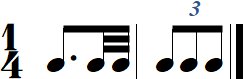
\includegraphics[scale=0.20]{pictures/score5.png}
%is encoded with the nested word $\langle \prec 0, \frac{3}{4}, \frac{7}{8} \succ \rangle %\langle \prec 1, \frac{4}{3}, \frac{5}{3}  \succ \rangle$
Another example is the other candidate
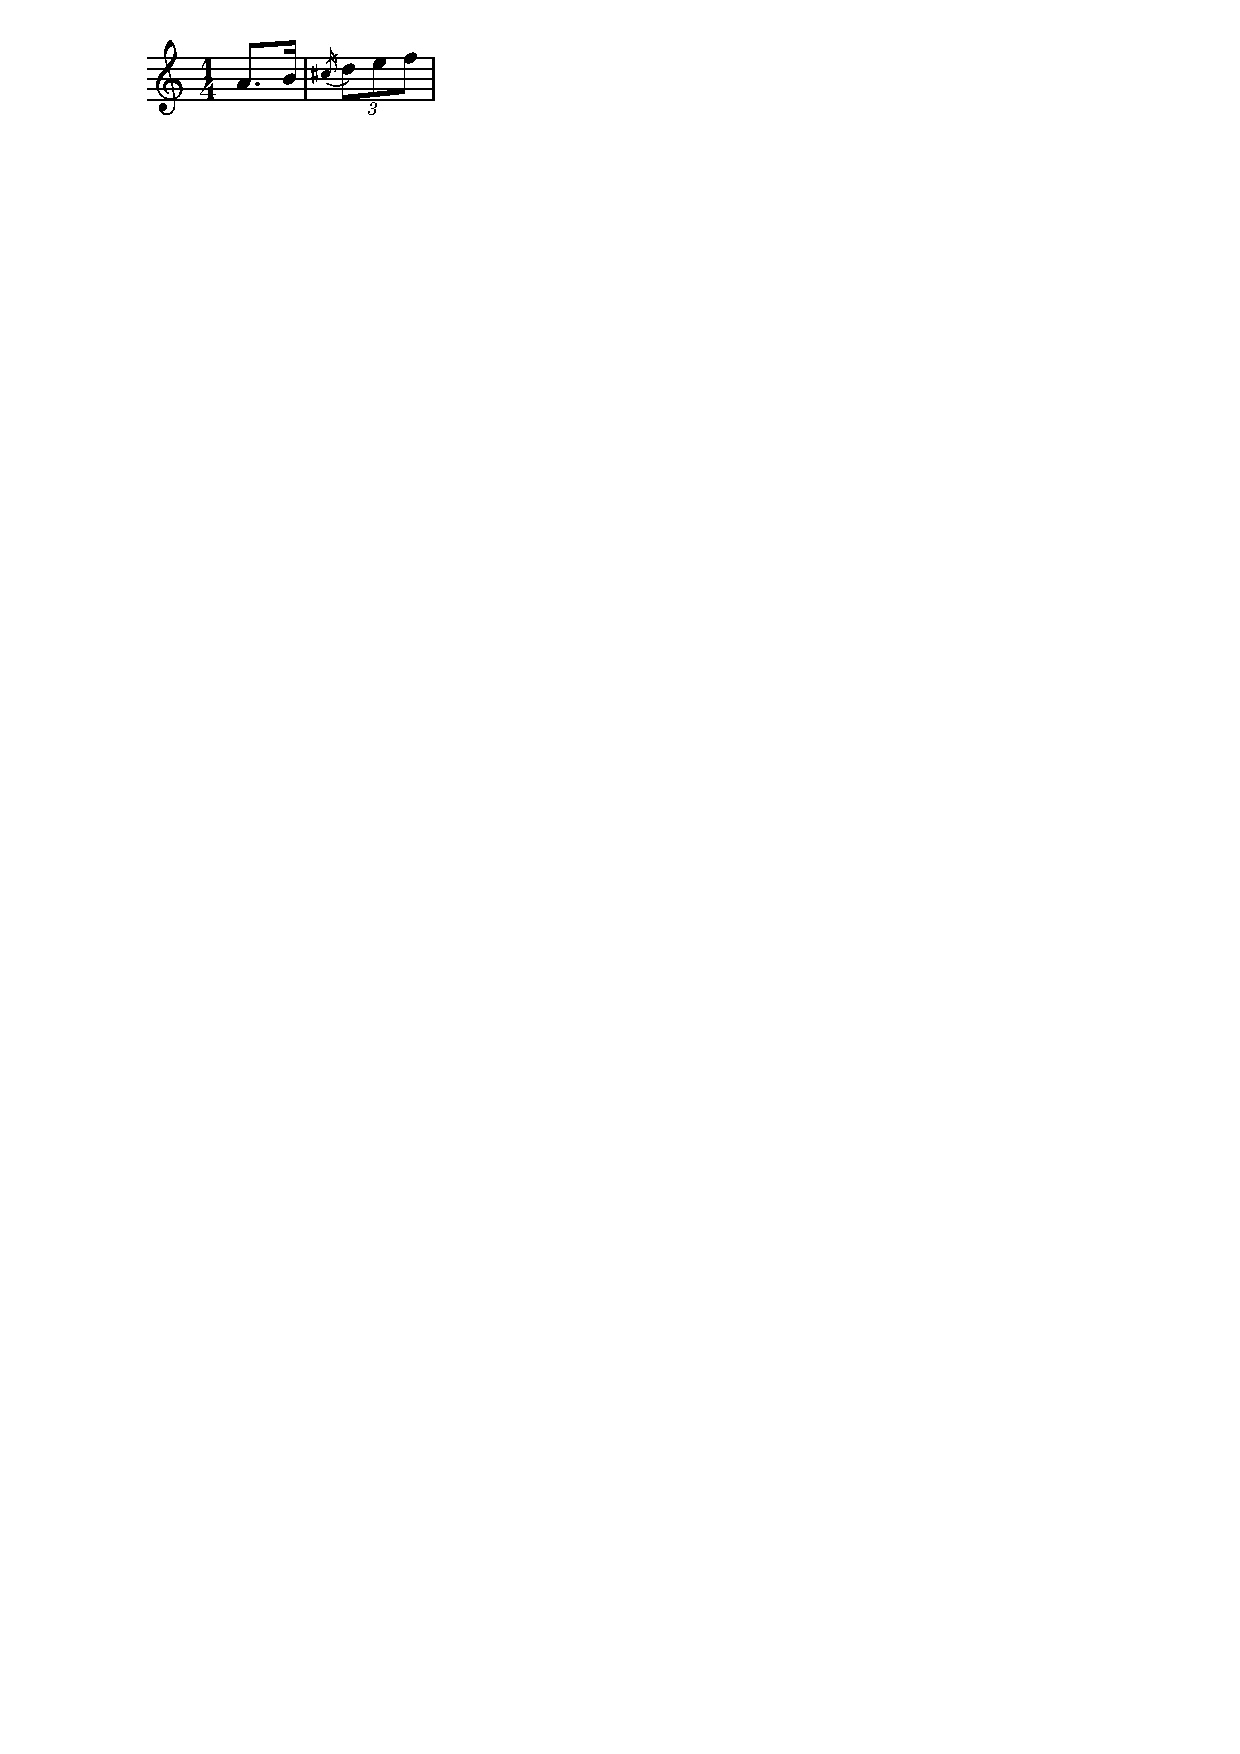
\includegraphics[scale=0.35,trim=0 5mm 0 0]{pictures/ex2.pdf}
of transcription of~$I$,
linearized into
$O' =$
$\ccall{\mathsf{m}}\tstamp{[0,1]}$,
$\ccall{2}\tstamp{[0,1]}$,
$\mbox{\footnotesize A4}\tstamp{0}$,
$\ccall{2}\tstamp{[\frac{1}{2},1]}$,
$-\tstamp{\frac{1}{2}}$,
$\mbox{\footnotesize B4}\tstamp{\frac{3}{4}}$,
$\creturn{2}\tstamp{1}$,
$\creturn{2}\tstamp{1}$,
$\ccall{\mathsf{m}}\tstamp{[1,2]}$,
$\ccall{3}\tstamp{[1,2]}$,
$\mbox{\footnotesize `C$\sharp$5`}\tstamp{1}$,
$\mbox{\footnotesize D5}\tstamp{1}$,
$\mbox{\footnotesize E5}\tstamp{\frac{4}{3}}$,
$\mbox{\footnotesize F5}\tstamp{\frac{5}{3}}$,
$\creturn{3}\tstamp{2}$,
$\creturn{\mathsf{m}}\tstamp{2}$,
$\creturn{\mathsf{m}}\tstamp{2}$
(see also Fig.~\ref{fig:score-tree}).
The symbol between quotes $\mbox{\footnotesize `C$\sharp$5`}$
represents an \emph{appogiatura}, %(grace-note),
\ie an ornamental note with theoretical duration~0.
\endex
\end{example}


\begin{definition}
A \emph{Symbolic Weighted Visibly Pushdown Automata} (\SWVPA)
over  $\Delta = \Deltai \uplus \Deltac \uplus \Deltar$, $\Semiring$ and $\bar\Phi$
is a tuple $A = \< Q, P, \init, \bar\wei, \final >$,
where $Q$ is a finite set of states,
$P$ is a finite set of stack symbols,
$\mathsf{in} : Q \to \Semiring$
(respectively $\mathsf{out} : Q \to \Semiring$)
are functions defining the weight for entering
(respectively leaving) a state,
and $\bar\wei$ is a sextuplet composed of the transition functions :
$\weii : Q \times P \times Q \to \Phici$,
$\weiei : Q \times Q \to \Phii$,
$\weic : Q \times P \times Q \times P \to \Phicc$,
$\weiec : Q \times P \times Q \to \Phic$,
$\weir : Q \times P \times Q \to \Phicr$,
$\weier : Q \times Q \to \Phir$.
%and
%$\weiex : Q \times Q \to \Phix$
%with $\mathsf{x} \in \{ \mathsf{i}, \mathsf{c}, \mathsf{r}\}$.
\end{definition}
%
As in Section~\ref{section:transducer},
we extend the above transition functions as follows
for every $q, q' \in Q$, $p \in P$,
$a \in \Deltai$,
$\call{c} \in \Deltac$,
$\return{r} \in \Deltar$,
overloading their names: % for simplicity:
\[
\begin{array}{lll}
\weii: Q \times [\Deltac \times P] \times \Deltai \times Q \to \Semiring &
\weii(q, c, p, a, q') = \eta_\mathsf{ci}(c, a) &
\mathrm{where~} \eta_\mathsf{ci} = \weii(q, p, q'),\\
%
\weiei: Q \times \Deltai \times Q \to \Semiring &
\weiei(q, a, q') = \phi_\mathsf{i}(a) &
\mathrm{where~} \phi_\mathsf{i} = \weiei(q, q').\\
%
\weic: Q \times [\Deltac \times P] \times  [\Deltac \times P] \times Q \to \Semiring &
\weic(q, c, p, \call{c'}, p', q') = \eta_\mathsf{cc}(c, \call{c'}) &
\mathrm{where~} \eta_\mathsf{cc} = \weic(q, p, p', q'),\\
%
\weiec: Q \times [\Deltac \times P] \times Q \to \Semiring &
\weiec(q, {\call{c}}, p', q') = \phi_\mathsf{c}({\call{c}}) &
\mathrm{where~} \phi_\mathsf{c} = \weiec(q, p, q').\\
%
\weir: Q \times [\Deltac \times P] \times \Deltar \times Q \to \Semiring &
\weir(q, {\call{c}},  p, {\return{r}}, q') = \eta_\mathsf{cr}({\call{c}},  {\return{r}}) &
\mathrm{where~} \eta_\mathsf{cr} = \weir(q, p, q'),\\
%
\weier: Q \times \Deltar \times Q \to \Semiring &
\weier(q, {\return{r}}, q') = \phi_\mathsf{r}({\return{r}}) &
\mathrm{where~} \phi_\mathsf{r} = \weier(q, q').\\
\end{array}
\]
The tuples in the definition domains of the above functions 
are also called \emph{transitions} of the \SWVPA.
We denote by $\src(\tau)$ (respectively $\snd(\tau)$) the first (respectively second) 
state component of a transition~$\tau$.
%
\noindent
%The intuition is the following for the above transitions.
Intuitively, $\weiei$, $\weiec$, and $\weier$ describe the cases where the stack is empty.
The transitions of $\weii$ and $\weiei$ both read an internal symbol~$a$ 
and change state from $q$ to $q'$, without changing the stack.
Moreover, $\weii$ reads a pair made of
${\call{c}} \in \Deltac$ and $p \in P$ on the top of the stack
($c$ is compared to $a$ by the weight function $\eta_\mathsf{ci} \in \Phici$).
%
\noindent
The transitions of $\weic$ and $\weiec$ read the call symbol $\call{c}'$,
push it to the stack along with $p'$, and change state from $q$ to to $q'$.
Moreover, $\weic$ reads ${\call{c}}$ and $p$ at the top of the stack
($c$ is compared to $c'$).
%and $\weiec$ applies iff the stack is empty.
%
\noindent
Finally, $\weir$ and $\weier$ read the return symbol $\return{r}$, and change state from $q$ to to $q'$.
Moreover, $\weir$ reads and pops from stack a pair made of $\call{c}$ and $p$
($\call{c}$ is compared to $\return{r}$).
%and $\weier$ applies iff the stack is empty.
%In this case, the weight function $\phi_\mathsf{r}$
%computes a value of matching between the call and return symbols $c$ and $r$.
%This value might be set to $\zero$ in order to express that the symbols do not match.

Formally, the computations of the automaton~$A$ are defined
with an intermediate function $\weight_A$, like in Section~\ref{sec:SWT}.
%
A configuration $q[\gamma]$
is composed of a state $q \in Q$
and a stack content $\gamma \in \Gamma^*$,
where $\Gamma = \Deltac \times P$.
Hence, $\weight_A$ is a function from
$[Q \times \Gamma^*] \times \Delta^* \times [Q \times \Gamma^*]$ into~$\Semiring$.
The empty stack is denoted by $\bot$, and the topmost
symbol is the last pushed pair.
%
The recursive definition of $\weight_A$
enumerates each of the six possible cases:
reading $a \in \Deltai$,
%\lydia{intro to func}
or $\call{c} \in \Deltac$, or $\return{r} \in \Deltar$,
for each possible state of the stack (empty or not).
%to add to $u \in {\Delta}^*$.
%\lydia{introduced the 6 cases}
\florent{shorter notation $cp$ for $\< c, p>$ ?}

\begin{align}
%\weight_A\bigl(\config{q}{\bot}, \varepsilon, \config{q}{\bot}) & = \one\label{eq:SWVPA-weight}\\
%\weight_A\bigl(\config{q}{\bot}, \varepsilon, \config{q'}{\gamma}) & = \zero
%\mathrm{~if~} q \neq q'\nonumber\\
%
\weight_A\bigl(\config{q}{\gamma}, \varepsilon, \config{q'}{\gamma'}) & = \one
\mathrm{~if~} q = q', \gamma =\gamma' = \bot
\mathrm{~and~} \zero \mathrm{~otherwise}\label{eq:SWVPA-weight}\\
%
\weight_A\bigl(\config{q}{\gamma}, u\, a,
               \configup{q'}{\<{\call{c}}, p>\stackup\gamma'}\bigr) & =
 {\displaystyle\bigoplus_{q'' \in Q}} 
  \weight_A\bigl(\config{q}{\gamma}, u,
                 \configup{q''}{\<{\call{c}}, p> \stackup \gamma'}\bigr) 
  \otimes \weii(q'', c, p, a, q') \nonumber\\
%
\weight_A\bigl(\config{q}{\gamma}, u\, a,
               \config{q'}{\bot}\bigr) & =
  {\displaystyle\bigoplus_{q'' \in Q}} 
   \weight_A\bigl(\config{q}{\gamma}, u, \config{q''}{\bot}\bigr)
   \otimes\weiei(q'', a, q')\nonumber\\
%
\weight_A\bigl(\config{q}{\gamma}, u\,{\call{c}'},
               \configup{q'}{\<{\call{c}'}, p'>\stackup \<{\call{c}}, p>\stackup \gamma'}\bigr) & =
 {\displaystyle\bigoplus_{\begin{array}{c}
                          \scriptstyle q'' \in Q\\[-1ex]
                          \scriptstyle p' \in P
                          \end{array}}}
 \weight_A\bigl(\config{q}{\gamma}, u,
                \configup{q''}{\<{\call{c}}, p>\stackup\gamma'}\bigr)
 \otimes \weic\bigl(q'', {\call{c}}, p, {\call{c}'}, p', q'\bigr)
\nonumber\\[1mm]
%
\weight_A\bigl(\config{q}{\gamma}, u\, {\call{c}},
               \config{q'}{\<{\call{c}}, p>}\bigr) & =
 {\displaystyle\bigoplus_{\begin{array}{c}
                          \scriptstyle q'' \in Q\\[-1ex]
                          \scriptstyle p \in P
                          \end{array}}}
 \weight_A\bigl(\config{q}{\gamma}, u,
                \config{q''}{\bot}\bigr)
 \otimes \weiec(q'', {\call{c}}, p, q')
\nonumber\\
%
\weight_A\bigl(\config{q}{\gamma}, u\,{\return{r}},
               \config{q'}{\gamma'}\bigr) & =
 {\displaystyle\bigoplus_{q'' \in Q}}
  \weight_A\bigl(\config{q}{\gamma}, u,
                 \configup{q''}{\<{\call{c}}, p>\stackup\gamma'}\bigr)
  \otimes \weir\bigl(q'', {\call{c}}, p, {\return{r}}, q'\bigr)\nonumber\\
%
\weight_A\bigl(\config{q}{\gamma}, u\,{\return{r}},
               \config{q'}{\bot}\bigr) & =
 {\displaystyle\bigoplus_{q'' \in Q}} 
          \weight_A\bigl(\config{q}{\gamma}, u,
                         \config{q''}{\bot}\bigr)
  \otimes \weier(q'', {\return{r}}, q')\nonumber
\end{align}
%\lydia{c p to <c, p>}
%
% and ${\call{c}}\, p\stacksep \gamma$
%denotes a stack where the pair made of ${\call{c}} \in \Deltac$ and $p \in P$ is the top symbol
%and $\gamma$ is the rest of stack.

\noindent
The weight associated by $A$ to $t \in \Delta^*$
is defined according to empty stack semantics:
%
\begin{equation}
A(t)  =
{\displaystyle\bigoplus_{q, q' \in Q}} \textstyle
\mathsf{in}(q) \mathop{\otimes}
\weight_A\bigl(\config{q}{\bot}, t, \config{q'}{\bot}\bigr)
\mathop{\otimes} \mathsf{out}(q')
\label{eq:SWVPA-value}
\end{equation}

\noindent
Every $\SWA$ $A = \< Q, \init, {\wei_1}, \final >$,
over $\Sigma$, $\Semiring$ and $\bar\Phi$
is a special case of $\SWVPA$
$\< Q, \emptyset, \init, \bar\wei, \final >$
over $\Delta$, $\Semiring$ and $\bar\Phi$
with $\Deltai = \Sigma$ and $\Deltac = \Deltar = \emptyset$,
and computing with an always empty stack:
$\weiei = \wei_1$ and all the other functions
of~$\bar\wei$ are the constant~$\zero$.

\begin{example} \label{ex:SWVPA}
\reviews{revision ex. needed. see rev. 3) and app. $\weic$, $\weir$, $\weii$ wrong.}
We consider a \SWVPA over the alphabet of Example~\ref{ex:nested-word} and with $P = Q$,
that expresses a weight related to the music notation,
or more precisely to its structural complexity.
Given a set of equivalent representations, we aim at choosing the simpler one, \ie the one with the smallest weight.

\lydia{We should find a better variable name than j... it does not render well in fractions}
Let's say the top of the stack is a tuple of the call~$\ccall{n}\tstamp{[\tau, \tau+\ell]}$ and a state $q$. Let's now consider a new call transition starting in state $q_{\frac{j}{n}}$, that is the $j$-th state of the $n$ sub-intervals of duration~$\frac{\ell}{n}$.
We thus read a new time-division symbol ~$\ccall{d}$ 
and compute the weight of the transition from $q_{\frac{j}{n}}$ to $q_{\frac{1}{d}}$, 
the first state after the new~$\ccall{d}$, reading on the top of the stack the pair
$\<\ccall{n}\tstamp{[\tau, \tau+\ell]}, q>$, 
and pushing $\<\ccall{d}\tstamp{\iota}, q_{\frac{j+1}{c}}>$ on top, or:
\(
\weic\bigl(q_{\frac{j}{n}},
           \ccall{n}\tstamp{[\tau, \tau+\ell]}, q,
           \ccall{d}\tstamp{\iota}, q_{\frac{j+1}{c}},
           q_{\frac{1}{d}} \bigr) = \alpha_d
\).
\lydia{is it ok to explain precisely this computation and not the others ? is it redundant with the explaniation before equation (5) ?}
\noindent
Reading the $k$-th musical event $\mu$ in this current sub-interval is computed with:
\(
\weii\bigl(q_{\frac{k}{d}},
           \ccall{d}\tstamp{[\tau, \tau+\ell]}, q_{\frac{j}{n}},
           \mu\tstamp{\tau + \frac{j\ell}{d}}, q_{\frac{k+1}{d}} \bigr) = \alpha_\mu
\).
Finally, this sub-interval will end after reading a return symbol $\creturn{d}$ and compute:
\(
\weir\bigl(q_{\frac{d}{d}},
           \ccall{d}\tstamp{[\tau, \tau+\ell]}, q_{\frac{i+1}{c}},
           \,\creturn{d}\tstamp{\tau + \ell}, q_{\frac{i+1}{c}} \bigr) = \one
\).
\noindent
We described earlier the special cases where the stack is empty, which applies for example when reading the first measure 
for which we only push $\<\ccall{\mathsf{m}}\tstamp{[0, 1]}, q_{\frac{1}{1}}>$ in the stack:
\(
\weiec\bigl(q_{\frac{1}{1}},
           \ccall{\mathsf{m}}\tstamp{[0, 1]}, q_{1/1},
           q_{1/1} \bigr) = \one
\).
In comparison, any other new measure would compute instead:
\(
\weic\bigl(q_{\frac{1}{1}},
          \ccall{\mathsf{m}}\tstamp{[\tau-1, \tau]}, q_{\frac{1}{1}},
          \ccall{\mathsf{m}}\tstamp{[\tau, \tau+1]}, q_{\frac{1}{1}},
          q_{\frac{1}{1}} \bigr) = \one
\).

Each transition thus has a weight computing an overall weight for one representation of music notation. 
When setting the weights, we decide which notation is preferred if possible. 
For example, let's say we want to prioritize tuplets over triplets, then we set $\alpha_2$ and $\alpha_3$ such as $\alpha_2 > \alpha_3$. In conclusion, a \SWVPA is capable of computing several representations of the same piece of music, allowing to choose the best one.
\endex
\end{example}

%\begin{example} \label{ex:SWVPA}
%\reviews{revision ex. needed. see rev. 3) and app. $\weic$, $\weir$, $\weii$ wrong.}
%We consider a \SWVPA over the alphabet of Example~\ref{ex:nested-word} and with $P = Q$
%that expresses a weight related to the music notation,
%or more precisely to its structural complexity.
%Given a set of equivalent representations, we aim at choosing the simpler one.
%
%Let's say the top of the stack is a tuple of the call~$\ccall{n}\tstamp{[\tau, \tau+\ell] and a state $q$. Let's now consider a new call transition starting in state $q_{\frac{j}{n}}$, that is the $j$-th state of the $n$ sub-intervals of duration~$\frac{\ell}{n}$.
%We thus read a new time-division symbol ~$\ccall{d}$ and compute the weight of the transition from q_{\frac{j}{n}} to q_{\frac{1}{d} (the first state after the new ~$\ccall{d}$), reading the top of the stack <\ccall{n}\tstamp{[\tau, \tau+\ell]}, q>, and pushing <\ccall{d}\tstamp{\iota}, q_{\frac{j+1}{c}}> on top, or:
%\(
%\weic\bigl(q_{\frac{j}{n}},
           %\ccall{n}\tstamp{[\tau, \tau+\ell]}, q,
           %\ccall{d}\tstamp{\iota}, q_{\frac{j+1}{c}},
           %q_{\frac{1}{d}} \bigr) = \alpha_d
%%\).
%
%\noindent
%Reading the $k$-th musical event $\mu$ in this current sub-interval is computed with:
%\(
%\weii\bigl(q_{{k}/{d}},
           %\ccall{d}\tstamp{[\tau, \tau+\ell]}, q_{\frac{j}{n}},
           %\mu\tstamp{\tau + \frac{j\ell}{d}}, q_{\frac{k+1}{d}} \bigr) = \alpha_\mu
%\).
%Finally, this sub-interval will end after reading a return symbol \creturn{d} which will compute the transition:
%\(
%\weir\bigl(q_{\frac{d}{d}},
           %\ccall{d}\tstamp{[\tau, \tau+\ell]}, q_{\frac{i+1}{c}},
           %\,\creturn{d}\tstamp{\tau + \ell}, q_{\frac{i+1}{c}} \bigr) = \one
%\).
%
%\noindent
%We described earlier the special cases where the stack is empty, which applies for example when reading the first measure for which we push <\ccall{\mathsf{m}}\tstamp{[0, 1]}, q_{1/1}>, but don't read anything on the stack:
%\(
%\weiec\bigl(q_{1/1},
 %          \ccall{\mathsf{m}}\tstamp{[0, 1]}, q_{1/1},
%           q_{1/1} \bigr) = \one
%\).
%In comparison, any other new measure would compute instead:
%\(
%\weic\bigl(q_{1/1},
%          \ccall{\mathsf{m}}\tstamp{[\tau-1, \tau]}, q_{1/1},
%          \ccall{\mathsf{m}}\tstamp{[\tau, \tau+1]}, q_{1/1},
%          q_{1/1} \bigr) = \one
%\).
%\endex
%\end{example}


%\subsection{Properties}
\medskip\noindent
Similarly to \VPA~\cite{AlurMadhusudan09nested}
and \SVPA~\cite{dAntonyAlur14SVPDA},
the class of \SWVPA is closed under the binary operators of the underlying semiring.
%
\begin{proposition}\label{prop:SWVPA-product}
Let $A_1$ and $A_2$ be two \SWVPA
over the same~$\Delta$, commutative~$\Semiring$ and effective~$\bar\Phi$.
There exist two effectively constructible $\SWVPA$
$A_1 \oplus A_2$ and $A_1 \otimes A_2$,
such that for every $s \in \Delta^*$,
$(A_1 \oplus A_2)(s) = A_1(s) \oplus A_2(s)$ and
$(A_1 \otimes A_2)(s) = A_1(s) \otimes A_2(s)$.
\end{proposition}
%
\begin{proof}
%We do a classical product construction, see Appendix~\ref{sec:product} for details.
%similar to the case of the Boolean semiring~\cite{dAntonyAlur14SVPDA}.
% !TEX root = main.tex
%
% Proof of Proposition product swVPA
%
We prove the closure under $\otimes$. 
The proof of the closure under $\oplus$ is similar.

Let $A_1 = \< Q_1, P_1, \init_1, \bar\wei_1, \final_1 >$
and $A_2 = \< Q_2, P_2, \init_2, \bar\wei_2, \final_2 >$.
The \SWVPA $A_1 \otimes A_2$ is built by a 
classical product construction.
%
It has a state set $Q = Q_1 \times Q_2$
and a auxiliary set of stack symbols $P = P_1 \times P_2$:
$A_1 \otimes A_2 = \< Q, P, \init_{1, \otimes}, 
         \bar\wei_{\otimes}, \final_{\otimes} >$.
The weight entering and leaving functions         
$\init_{\otimes}$, $\final_{\otimes}$
and the sextuplet of transition functions $\bar\wei_{\otimes}$
are defined 
using the label-theory operators of Section~\ref{section:symbols}.
They will simulate the synchronized behaviour of $A_1$ and $A_2$.
%
For all $\< q_1, q_2>, \< q'_1, q'_2> \in Q$ 
and $\< p_1, p_2>, \< p'_1, p'_2> \in P$:
\[
\begin{array}{lcl}
\init_{\otimes}\bigl(\< q_1, q_2>\bigr) & = & \init_{1}(q_1) \otimes \init_{2}(q_2)\\
\final_{\otimes}\bigl(\< q_1, q_2>\bigr) & = & \final_{1}(q_1) \otimes \final_{2}(q_2)\\
%
\wei_{\mathsf{i}, \otimes}\bigl(\< q_1, q_2>, \<p_1, p_2>, \<q'_1, q'_2>\bigr) & = &
\wei_{\mathsf{i}, 1}(q_1, p_1, q'_1) \otimes \wei_{\mathsf{i}, 2}(q_2, p_2, q'_2)\\
%
\weie[\mathsf{i}, \otimes]\bigl(\< q_1, q_2>, \<q'_1, q'_2>\bigr) & = &
\weie[\mathsf{i}, 1](q_1, q'_1) \otimes \weie[\mathsf{i}, 2](q_2, q'_2)\\
%
\wei_{\mathsf{c}, \otimes}\bigl(\< q_1, q_2>, \<p_1, p_2>, \<q'_1, q'_2>, \<p'_1, p'_2>\bigr) & = &
\wei_{\mathsf{c}, 1}(q_1, p_1, q'_1, p'_1) \otimes \wei_{\mathsf{c}, 2}(q_2, p_2, q'_2, p'_2)\\
%
\weie[\mathsf{c}, \otimes]\bigl(\< q_1, q_2>, \<p_1, p_2>, \<q'_1, q'_2>\bigr) & = &
\weie[\mathsf{c}, 1](q_1, p_1, q'_1) \otimes \weie[\mathsf{i}, 2](q_2, p_2, q'_2)\\
%
\wei_{\mathsf{r}, \otimes}\bigl(\< q_1, q_2>, \<p_1, p_2>, \<q'_1, q'_2>\bigr) & = &
\wei_{\mathsf{r}, 1}(q_1, p_1, q'_1) \otimes \wei_{\mathsf{r}, 2}(q_2, p_2, q'_2)\\
%
\weie[\mathsf{r}, \otimes]\bigl(\< q_1, q_2>, \<q'_1, q'_2>\bigr) & = &
\weie[\mathsf{r}, 1](q_1, q'_1) \otimes \weie[\mathsf{i}, 2](q_2, q'_2)\\
\end{array}
\]






\qed
\end{proof}
\noindent
%We present now a procedure for searching, for a~$\SWVPA$ $A$,
%a word %$w \in \Delta^*$
%of minimal weight for~$A$.
We present now a procedure for searching a word of minimal weight for a~$\SWVPA$~$A$.
%as stated in the following proposition. %\wrt~$\leq_\oplus$,
%It requires the following property of label theories.
%
\begin{proposition}\label{th:best-search}
For a \SWVPA $A$
over $\Delta$,
$\Semiring$ commutative, bounded, total and complete, %semiring
and $\bar\Phi$ effective, %and $k$-convex, % label theory,
one can construct in PTIME a word $t \in \Delta^*$
such that $A(t)$ is minimal \wrt the natural ordering $\leq_\oplus$ for $\Semiring$.
\end{proposition}
%\florent{total?}
%
Let $A = \< Q, P, \init, \bar\wei, \final >$.
%
We propose first a method for %Dijkstra-like algorithm 
computing,
for every $q, q' \in Q$,
the minimum, \wrt $\leq_\oplus$, of the function
$\beta_{q, q'} : t \mapsto \weight_A(\config{q}{\bot}, t, \config{q'}{\bot})$.
Let us denote by $b_\bot(q, q')$ this minimum.
\florent{it exists by effectiveness of label th. ?}
%
By definition of $\leq_\oplus$, and since $\Semiring$ is total,
\reviews{1) $\Semiring$ total $\to$ $\Semiring$ extremal}
it holds that
(the infinite sum in~\eqref{eq:bbot} is well defined since $\Semiring$ is complete):
%
\begin{equation}\label{eq:bbot}
  b_\bot(q, q') = \bigoplus_{t\in \Delta^*}
  \textstyle
  \weight_A\bigl(\config{q}{\bot}, t, \config{q'}{\bot}\bigr).
\end{equation}
%
Following~\eqref{eq:SWVPA-value}, and the associativity, commutativity
and distributivity for~$\otimes$ and~$\oplus$, the minimum of~$A(t)$ is:
\begin{equation}\label{eq:min}
{\displaystyle\bigoplus_{t\in \Delta^*}} A(t)
=
{\displaystyle\bigoplus_{t\in \Delta^*}}
{\displaystyle\bigoplus_{q, q' \in Q}} \textstyle
\mathsf{in}(q) \mathop{\otimes}
\beta_{q, q'}(t)
\mathop{\otimes} \mathsf{out}(q')
=
{\displaystyle\bigoplus_{q, q' \in Q}} \textstyle
\mathsf{in}(q) \mathop{\otimes}
b_\bot(q, q')
\mathop{\otimes} \mathsf{out}(q')
\end{equation}

\noindent
Hence, in order to prove Proposition~\ref{th:best-search}, 
it is sufficient to show that we can compute $b_\bot(q, q')$ for all $q, q' \in Q$. 
For this purpose, we shall consider an auxiliary function $b_\top :  Q \times P \times Q \to \Phic$
that corresponds to the cases where the stack of $A$ is not empty.
%
Intuitively, $b_\top(q, p, q')$ is a function of~$\Phic$,
mapping every $c \in \Deltac$ to
the minimum weight of a computation of~$A$
starting in state~$q$, 
with a non-empty stack $\gamma' = \<c, p> \, \gamma \in \Gamma^+$,
and ending in state~$q'$ with the same stack~$\gamma'$,
such that
the computation does not pop the pair $\<c, p>$ at the top of $\gamma'$
(\ie~$\gamma'$ is left untouched during the computation).
However, the computation can read $\<c, p>$ at the top of $\gamma'$,
and can also push another pair $\< c', p'> \in \Gamma$ on top of $\gamma'$,
following the third case 
in the definition \eqref{eq:SWVPA-weight} of $\weight_A$ (call symbol).
The pair $\< c', p'>$ can be popped later, during the computation from $q$ to $q'$,
following the fifth case of \eqref{eq:SWVPA-weight} (return symbol).
%However, it cannot apply one of the two last cases (return symbol and empty stack)
%when the current stack is $\gamma$.
%pop symbols in $\gamma$.
%
% Note that having a stack reduced to such a symbol makes impossible the application of the
% two last cases in the definition of $\weight_A$ (return symbol and empty stack).
% However, it is possible to apply the two first cases
% (internal symbol or call symbol, with a push on the top of $\top$).
%
Formally, in order to define~$b_\top$, we consider
a fresh stack symbol $\top \notin \Gamma$,   %which does not belong to $\Gamma$,
representing the above untouched stack, and let:
%
\begin{equation}\label{eq:btop}
  b_\top(q, p, q') : c \mapsto \bigoplus_{s\in \Delta^*}
  \textstyle
  \weight_A\bigl(\configup{q}{\< c, p> \stackup \top }, s, \configup{q'}{\<c, p> \stackup \top}\bigr)
\quad
\mathrm{~for~all~} c \in \Deltac
\end{equation}
%
%By definition of $\weight_A$ in \eqref{eq:SWVPA-weight},
%using the symbol $\top$ for the part of the stack below $\<c, p>$
%(\ie the substack $\gamma$ in the above $\gamma' = \<c, p> \, \gamma$)
%ensures that this part is not touched during the computation.
% there cannot be a pop of $\<c, p>$ followed by a push of $\<c, p>$
% because it is not possible to push over $\top$ (push read the top of stack).
%
This ensures in particular that the subword
read during the computation is well parenthesized
(every symbol in $\Deltac$ has a matching symbol in $\Deltar$).

% Note that having a stack reduced to such a symbol makes impossible the application of the
% two last cases in the definition of $\weight_A$ (return symbol and empty stack).
% However, it is possible to apply the two first cases
% (internal symbol or call symbol, with a push on the top of $\top$).

%The term $\config{q}{\bot}, s, \config{q'}{\bot}$
%of this sum is the central expression in
%the definition \eqref{eq:weightA} of $A(s_0)$, for the minimum $s_0$
%of the function $\weight_A$.


\medskip
% !TEX root = main.tex
%

\florent{New Algorithm for best-search}
We shall compute the values of the functions $b_\bot$ and $b_\top$
by search of shortest paths in a $\Semiring$-labeled graph $\G_A$
associated to the \SWVPA $A$. 
This graph is defined by $\G_A = \< V_A, E_A, \eta_A >$, 
with set of vertices $V_A = (Q \times Q) \cup (Q \times P \times Q)$,
set of edges $E_A = V_A \times V_A$
(an edge $\< v_1, v_2>$, with $v_1, v_2 \in V_A$ is denoted by $v_1 \to v_2$),
and with an edge labelling  
$\eta_A : E_A \to \Semiring$ defined by, %as follows,
for $q_0, q_1, q_2, q_3 \in Q$, $p, p' \in P$:
%
\[
\begin{array}{rclcl}
%
\< q_0, q_1> & \to & \< q_0, q_2> & \mapsto &
\bigoplus_{\Deltai} \weiei(q_1, q_2) \oplus \bigoplus_{\Deltar} \weier(q_1, q_2)\\
%
\< q_1, p, q_2> & \to & \<q_0, q_3> & \mapsto &
\bigoplus_{\Deltac} \bigl[ \weiec(q_0, p, q_1) \otimes \bigoplus^2_{\Deltar} \weir(q_2, p, q_3)\bigr]\\ 
%
%\< q_0, p, q_1> & \to & \< q_0, p, q_2> & : &
%\bigoplus_{\Deltai} \weii(q_1, p, q_2)\\
%
\< q_1, p', q_2> & \to & \< q_0, p, q_3> & \mapsto &
{\displaystyle\bigoplus_{q_0=q_1}}
{\displaystyle\bigoplus_{p=p'}}
 \bigoplus_{\Deltai} \weii(q_2, p, q_3)\\
 & & & & 
\qquad\quad 
\oplus \bigoplus^2_{\Deltac} \bigl[ \weic(q_0, p, p', q_1) \otimes_2 {\bigoplus_{\Deltar}} \weir(q_2, p', q_3) \bigr]\\
%
\end{array}
\]
%Removing from $\G_A$ every edge $e \in E_A$ such that $\eta(e) = \zero$ 
%is preserving the results below.
%
A \emph{path} of $\G_A$ is a sequence $\pi = v_0,\ldots, v_n \in V^*_A$,
it is called \emph{safe} when $v_0$ has the form $\< q, q>$ for some $q \in Q$, 
and $n_v$ is called $\last(\pi)$.
%
A path $\pi$ is assigned a weight value $\weight(\pi) \in \Semiring$ which is the product by $\otimes$ 
of the weights of the edges involved in the path.
More precisely, for all $q, q' \in Q$ and $p \in P$, we let 
$\weight(\< q, q' > ) = \one$ if $q = q'$, and $\zero$ otherwise, 
$\weight(\< q, p, q' > ) = \zero$ and 
for all $n \geq 1$, 
$\weight(v_0,\ldots, v_n) = \weight(v_0,\ldots, v_{n-1}) \otimes \eta_A(v_{n-1} \to v_{n})$.
%$\weight(\pi) = \bigotimes_{i=1}^{n} \eta(v_{i-1} \to v_i)$.

%Intuitively, 
\begin{lemma}[Correctness]
For all safe path~$\pi$ of~$\G_A$,  %with $\src(\pi) = \<q_0, q_0>$,
%with last element $v$, \\
($i$) if $\last(\pi) = \< q, q'>$, %with $q, q' \in Q$, 
then there exists $u \in \Delta^*$ such that 
$\weight_A(q[\bot], u, q'[\bot]) = \weight(\pi)$,\\
%
($ii$) if $\last(\pi) = \< q, p, q'>$, %with $q, q' \in Q$, $p\in P$, 
then there exists $v \in \Delta^*$ such that \\
${\displaystyle\bigoplus_{c \in \Deltac}}
 \weight_A\bigl(\configup{q}{\< c, p> \stackup \top }, v, \configup{q'}{\<c, p> \stackup \top}\bigr)
 = \weight(\pi)$.
\end{lemma}
%
\begin{proof}
We prove ($i$) and ($ii$) simultaneously by induction on the length $|\pi|$ of the path $\pi$.

\noindent
The base case $|\pi| = 1$ is a direct consequence of the definition of weight of paths of length 1
and the first line of \eqref{eq:SWVPA-weight}.

\noindent
If $\pi = v_0,\ldots, v_n$ with $n \geq 1$, 
let us do a case analysis on the edge $v_{n-1} \to v_n$.
...
\qed
\end{proof}



\begin{lemma}[Completeness] \label{lem:algo-completeness}
For all $q, q' \in Q$, $p\in P$, 
($i$) there exists a safe path~$\pi$ of~$\G_A$ such that
%such that $\src(\pi) = \<q_0, q_0>$ for some $q_0 \in Q$, 
$\last(\pi) = \< q, q'>$,
and $\weight(\pi) = b_\bot(q, q')$, 
($ii$) there exists a safe path $\pi'$ of $\G_A$ 
such that $\last(\pi') = \< q, p, q'>$,
and $\weight(\pi') = \bigoplus_\Deltac b_\top(q, p, q')$.
\end{lemma}
%
\begin{proof}
By associativity, commutativity and distributivity for $\Semiring$,
\eqref{eq:bbot} can be rewritten into the form, unfolding~\eqref{eq:SWVPA-weight}:
%
\begin{equation}\label{eq:bbot-unfold}
b_\bot(q, q') = 
\bigoplus_{t\in \Delta^*} 
\bigoplus_{\begin{array}{c}
           \scriptstyle q_0,\ldots, q_n \in Q\\
           \scriptstyle p_{i},\ldots, p_{k} \in P
           \end{array}}
\bigotimes_{i=1}^n w_i(\tau_i)           
\end{equation}
%
where $n$ is the length of $t$, $k \leq n$,
$q_0 = q$, $q_n = q'$, 
for all $1 \leq i < n$, 
$w_i$ is one of the functions of $\bar\wei$,
$\tau_i$ is a transition of $A$ and
$\src(\tau_i) = q_{i-1}$, $\snd(\tau_i) = q_i$.
%
Since $\Semiring$ is total, there exists finite sequences as above such that
\( b_\bot(q, q') = \bigotimes_{i=i}^n w_i(\tau_i)\).
%
There might exists, for $q$ and $q'$,
several finite sequences~$\bar\tau$ and~$\bar{w}$ as above, 
let us choose arbitrarily one of minimal length~$n$. 
This integer $n$ will be denoted $n_{q, q'}$ in the following.
%We represent a computation of $A$ on $t$ by a sequence $\rho$ of its transitions, 

Similarly, following~\eqref{eq:btop} and~\eqref{eq:SWVPA-weight}, 
$\bigoplus_\Deltac b_\top(q, p, q')$ can be put in the form:
%
\begin{equation}\label{eq:btop-unfold}
{\textstyle\bigoplus_\Deltac} b_\top(q, p, q') = 
{\textstyle\bigoplus_\Deltac} \bigoplus_{t\in \Delta^*} 
\bigoplus_{\begin{array}{c}
           \scriptstyle q_0,\ldots, q_n \in Q\\
           \scriptstyle p_{i},\ldots, p_{k} \in P
           \end{array}}
\bigotimes_{i=1}^n w_i(\tau_i)           
\end{equation}
%
and hence 
\( {\textstyle\bigoplus_\Deltac} b_\top(q, p, q') = \bigotimes_{i=i}^n w_i(\tau_i) \),
using $c \in \Deltac$ that minimize the function in rhs of~\eqref{eq:btop-unfold}.
We denote the smallest $n$ as above by $n_{q, p, q'}$.

\noindent
We show now the existence of a path $\pi$ of Lemma~\ref{lem:algo-completeness}, 
by simultaneous induction on $n_{q, q'}$ and $n_{q, p, q'}$.

The base case, $n = 0$ corresponds to $t = \varepsilon$. 
In this case, by~\eqref{eq:SWVPA-weight}, $b_\top(q, p, q') = \zero$,
$b_\bot(q, q) = \one$ and $b_\bot(q, q') = \zero$ if $q \neq q'$.

\noindent
For $n = n_{q, q'} > 0$, let $\bar\tau$ and~$\bar{w}$
be the sequences associated to $q$ and $q'$ as above.
Let us do a case analysis of $w_n$.



 

\end{proof}





%

\begin{algorithm}
\SetKw{Extract}{extract}
\SetKw{Update}{update}

\textbf{initially} let $\Q = (Q \times Q) \cup (Q \times P \times Q)$,
and let $d_\bot(q_1, q_2) = d_\top(q_1, p, q_2) = \one$
if $q_1 = q_2$ and $d_\bot(q_1, q_2) = d_\top(q_1, p, q_2) = \zero$ otherwise$\;$

\smallskip\noindent
\While{$\Q \neq \emptyset$}{

%\noindent\quad
\Extract $\< q_1, q_2>$ or $\< q_1, p, q_2>$ from $\Q$
%
%\noindent\quad
such that $d_\bot(q_1, q_2)$, 
resp. $\bigoplus_{\Deltac} d_\top(q_1, p, q_2)$, is minimal in $\Semiring$ \wrt $\leq_\oplus$$\;$

%\noindent\quad
%\textbf{for all} $q_0, q_3 \in Q$
\Update $d_\bot$ if $\< q_1, q_2>$ was extracted (Figure~\ref{fig:best-update-bottom}), or \\
\Update $d_\top$ if $\< q_1, p, q_2>$ was extracted (Figure~\ref{fig:best-update-top}).$\;$
}
\caption{Best search for \SWVPA}
\label{algo:Dijkstra}
\end{algorithm}

\textbf{Proof of correctness}

To prove that the algorithm does compute the word with the best weight, we use the following invariant :
$$
\<q_1, q_2> \notin Q \iff d_{\bot}(q_1, q_2) = b_{\bot}(q_1, q_2)
$$
In other words, a tuple $\<q_1, q_2>$ is removed from the queue during an iteration only when $d_{\bot}(q1, q2)$ has its minimal value.

Initialization : Before the while loop, no tuple has been extracted from the queue, so the invariant is trivially true.

Recursion : 

Let's show by contradiction that at each iteration of the while loop, for the tuple $\<q, q'>$ extracted from Q we have:
$$
d_{\bot}(q, q') = b_{\bot}(q, q'), 
$$


Let's consider the states $q_0$, $q_1$, $q_2$ and $q_3$ $\in Q$ such as they form a path $q$ ~...~>$q_0$ -> $q_1$ -> $q_2$ -> $q_3$ ~..~> $q'$.

We take $\<q_0, q_1>$ as the first tuple to be removed from the queue. Then when $\<q_0, q_1>$ is extracted from the queue, the algorithms updates $d_{\bot}(q_0, q_2)$ and $d_{\bot}(q_0, q_3)$. Thus, we have:
$$
d_{\bot}(q_0, q_2) \geq b_{\bot}(q_0, q_1) \\
d_{\bot}(q_0, q_3) \geq b_{\bot}(q_0, q_1)
$$
Let's show that it is true for each update possible, shown in Figure 3. TODO

Let $\<q_0, q_3>$ be the first tuple for which the invariant is false:
$$
For \<q_0, q_3> \notin Q, d_{\bot} (q_0, q_3) \neq b_{\bot} (q_0, q_3)
$$
Since $d_{\bot}(q_0, q_2)$ has to be computed to compute $d_{\bot}(q_0, q3)$, and because the invariant is true for  $d_{\bot}(q_0, q_2)$ we can say:
$$
d_{\bot}(q_0, q_2) = b_{\bot}(q_0, q_2) \\
d_{\bot}(q_0, q_2) \leq b_{\bot}(q_0, q_3) \\
\\d_{\bot}(q_0, q_2) \leq d_{\bot}(q_0, q_3) \\
$$
 However, when $\<q_0, q_3>$ was extracted, $\<q_0, q_2>$ was still in $Q$. Thus, by definition 
$$
d_{\bot}(q_0, q_2) \geq d_{\bot}(q_0, q_3) \\
$$
Then the two inequalities are actually equal : 
$$
d_{\bot}(q_0, q_2) = b_{\bot}(q_0, q_2) = d_{\bot}(q_0, q_3) = b_{\bot}(q_0, q_3) \\
$$
We find that $d_{\bot}(q_0, q_3) = b_{\bot}(q_0, q_3)$, so by contradiction, we find that indeed $d_{\bot}(q_0, q_3) = b_{\bot}(q_0, q_3)$ iff 
$\<q_0, q_3> \notin Q$.


Termination: TODO 


Algorithm~\ref{algo:Dijkstra} constructs iteratively, using a priority queue $\Q$, 
two markings
$d_\bot : Q \times Q \to \Semiring$ and
$d_\top : Q \times P \times Q \to \Phic$,
%of the triplets $\<q, \sigma, q'>$
%of states of $A$ by weight values in $\Semiring$,
that converge eventually to $b_\top$ and $b_\bot$. 
%
\florent{intuition sur update en commentaire}
%Intuitively, in the update defined in Figure~\ref{fig:best-update},
%we assume that the values of $d_\bot$ and $d_\top$ are definitely 
%fixed for every tuplet which has been extracted from the queue $\Q$ 
%(like in particular $\<q_1, q_2>$ or $\< q_1, p, q_2>$ when the algorithm calls this update), 
%and we use these values 
%(and the functions $w$ of transitions) 
%in order to update the values of $d_\bot$ and $d_\top$ 
%on the other tuplets (those which are still in the queue $\Q$).
%
\florent{explication Fig.~\ref{fig:best-update} (update) suivant cas de \eqref{eq:SWVPA-weight}?}
\florent{The infinite sums in the updates of $d$ in Algorithm~\ref{algo:Dijkstra},
 Figure~\ref{fig:best-update} are well defined since~$\Semiring$ is complete.}
%
% COMPLEXITY
%The algorithm performs $2.|Q|^2$ iterations until $P$ is empty,
%and each iteration has a time complexity $O(|Q|^2 . |P|)$.
%\florent{complexity: detail with and states?}
%That gives a time complexity $O(|Q|^4 . |P|)$.
%It can be reduced by implementing $P$ as a priority queue,
%prioritized by the value returned by $d$.
%** where  $T$ is the worst time complexity for an oracle computing the values
%of Definition~\ref{def:effective}.
%$|Q|^3.\log(|Q|^2)$
%
%Algorithm~\ref{algo:Dijkstra}
It terminates in PTIME (when $\Q$ is empty), 
and its correctness is ensured by~\eqref{eq:min} and  
the following invariants: 
$\< q_1, q_2> \notin \Q$ iff $d_\bot(q_1, q_2) = b_\bot(q_1, q_2)$, 
and $\< q_1, p, q_2> \notin \Q$ iff 
$\bigoplus_{\Deltac} d_\top(q_1, p, q_2) = \bigoplus_{\Deltac} b_\top(q_1, p, q_2)$.
\florent{(see Appendix~\ref{sec:bestsearch}).}
%of Algorithm~\ref{algo:Dijkstra}.

\begin{figure}[ht]
\(
\begin{array}{lcl}
\multicolumn{3}{l}{%
 \mbox{For~every}\  q_0, q_3 \in Q,}\\[1mm] % if $\< q_1, p, q_2> \notin \Q$
%
d_\bot(q_0, q_3) & \opluseq &
  d_\bot(q_0, q_2) \otimes
  \bigoplus_{\Deltai} \weiei(q_2, q_3)\ 
  \mathrm{if~} \< q_0, q_2> \notin \Q \\
%
d_\bot(q_0, q_3) & \opluseq &
  {\bigoplus_{\Deltac}}
  \bigl(
  \weiec(q_0, p, q_1) \otimes
   d_\top(q_1, p, q_2) \otimes
  \bigoplus^2_{\Deltar} \weir(q_2, p, q_3)\bigr)\ 
  \mathrm{if~} \< q_1, p, q_2> \notin \Q \\
%
d_\bot(q_0, q_3) & \opluseq &
  d_\bot(q_0, q_2) \otimes
  \bigoplus_{\Deltar} \weier(q_2, q_3)\ 
  \mathrm{if~} \< q_0, q_2> \notin \Q \\ 
%
d_\bot(q_0, q_3) & \opluseq &
  d_\bot(q_0, q_2) \otimes d_\bot(q_2, q_3)\  
  \mathrm{if~} \< q_0, q_2>\notin \Q, \< q_2, q_3> \notin \Q \\[-1mm]
\end{array}
\)
\caption{\textbf{update} $d_\bot$ (Algorithm~\ref{algo:Dijkstra}).}
\label{fig:best-update-bottom}
\end{figure}
%

\begin{figure}[ht]
\(
\begin{array}{lcl}
\multicolumn{3}{l}{%
 \mbox{For~every}\  q_0, q_3 \in Q\ \mbox{and}\ p \in P,}\\[1mm] % if $\< q_1, p, q_2> \notin \Q$
d_\top(q_0, p, q_3) & \opluseq &
  d_\top(q_0, p, q_2) \otimes
  \bigoplus_{\Deltai} \weii(q_2, p, q_3)\
  \mathrm{if~} \< q_0, p, q_2> \notin \Q \\
%\multicolumn{3}{l}{\quad
%\mathrm{where~} \weii(q_2, p, q_3)_a \in \Phic
%\mathrm{~is~the~partial~application~}
%x_c \mapsto \weii(q_2, x_c, p, a, q_3)}\\
d_\top(q_0, p, q_3) & \opluseq &
  {\bigoplus^2_{\Deltac}}
  \bigl[ \bigl( \weic(q_0, p, p', q_1) \otimes_2
  d_\top(q_1, p', q_2) \bigr) \otimes_2
  {\bigoplus_{\Deltar}} \weir(q_2, p', q_3) \bigr]\
  \mathrm{if~} \< q_1, p', q_2> \notin \Q \\
%\multicolumn{3}{l}{\quad
%\mathrm{where~} \weic(q_0, p, p', q_1)_{c'} \in \Phic
%\mathrm{~is~the~partial~application~}
%x_c \mapsto \weic(q_0, p, x_c, c', p', q_1)}\\[2pt]
%
d_\top(q_0, p, q_3) & \opluseq &
  d_\top(q_0, p, q_2) \otimes d_\top(q_2, p, q_3)\ 
  \mathrm{if~} \< q_0, p, q_2> \notin \Q, \< q_2, p, q_3> \notin \Q \\[-1mm]
\end{array}
\)
%$\weii(q_2, p, q_3)_a \in \Phic$, for $a \in \Deltai$,
%is the partial application
%$x_c \mapsto \weii(q_2, x_c, p, a, q_3)$.
%
%$\weic(q_0, p, p', q_1)_{c'} \in \Phic$, for $c' \in \Deltac$,
%is the partial application
%$x_c \mapsto \weic(q_0, p, x_c, c', p', q_1)$.
%\caption{Update $d_\bot$ with $\<q_1, q_2>$ or $d_\top$ with $\< q_1, p, q_2>$.}
\caption{\textbf{update} $d_\top$ (Algorithm~\ref{algo:Dijkstra}).}
\label{fig:best-update-top}
\end{figure}
%
%\noindent
%** effectively computable by hypothesis that the label theory is effective**
%\florent{REVOIR}
Thanks to the hypothesis that $\bar\Phi$ is effective, 
it is possible to construct during the iteration a witness word
for Proposition~\ref{th:best-search}, 
\ie a word $t \in \Delta^*$ with a minimal weight $A(t)$ \wrt~$\leq_\oplus$.

%we require the additional property of convexity of weight functions.***
%using the second requirement in Definition~\ref{def:effective}.


 % former version




%%%%%%%%%%%%%%%%%%%%%%%%%
\section{Symbolic Weighted Parsing}
\label{sec:parsing}
%% see parse-tree.tex for a definition with parse tree (instead of nested words)

Let us now apply the models and results of the previous sections %in order to define
to the problem of parsing over an infinite alphabet. %appropriate
%
%\subsection{Definition}
%
Let~$\Sigma$
and~$\Delta = \Deltai \uplus \Deltac \uplus \Deltar$
be countable input and output alphabets,
let $\< \Semiring, \oplus, \zero, \otimes, \one>$ be a
commutative, bounded, total and complete %\florent{total?} 
semiring and let $\bar\Phi$ be an effective label theory over $\Semiring$,
containing $\Phi_\Sigma$, $\Phi_{\Sigma, \Deltai}$, as well as
$\Phii$, $\Phic$, $\Phir$, $\Phicr$
(following the notations of Section~\ref{sec:SWVPA-def}).
%
\noindent
We assume to be given the following input:
\begin{description}
\item[--] a \SWT $T$ over $\Sigma$, $\Deltai$, $\Semiring$, and $\bar\Phi$,
defining a measure %between words
$T: \Sigma^* \times \Deltai^* \to \Semiring$,

\item[--] a \SWVPA $A$ over $\Delta$, $\Semiring$, and $\bar\Phi$,
defining a measure $A: \Delta^* \to \Semiring$,
%a \SWVPA $A$ over $\Delta$, and $\Semiring$, defining a series of nested words
%      $A : \Delta^* \to \Semiring$,
\item[--] an input word $s \in \Sigma^*$.
\end{description}
%
For every $u \in \Sigma^*$ and $t \in \Delta^*$, let
\(d(u, t) = T\bigl(u, t|_\Deltai \bigr)\),
where $t|_\Deltai \in \Deltai^*$ is the projection of $t$ onto~$\Deltai$,
obtained from $t$ by removing all symbols in $\Delta \setminus \Deltai$.
%
\noindent
\emph{Symbolic weighted parsing} is the problem,
given the above input,
to find $t \in \Delta^*$ %nested word $t \in \Delta$
minimizing \( d(s, t) \otimes A(t)\)
\wrt $\leq_\oplus$,
\ie s.t. %such that: %Hence, it is the problem of finding
%
\begin{equation}\label{eq:distance-lang}
d(s, t) \otimes A(t) = \displaystyle\bigoplus_{u \in \Delta^*} d(s, u) \otimes A(u)
\end{equation}
%
Following the terminology of~\cite{Mohri03ijfcs},
$\SW$-parsing is the problem of computing
the distance~\eqref{eq:distance-lang} between the input string~$s$ 
and the weighted language over the output alphabet defined by~$A$,
and returning a witness~$t$.

\begin{example}[Symbolic Weighted Parsing and the transcription problem]
Applied to the music transcription problem, the above formalism
is interpreted as follows:
%
\begin{itemize}
\item The input word is $I$ of Example~\ref{ex:running}.
\item The \SWT $T$ evaluates a ``fitness measure'' expressing
    a correspondence between a performance and a nested representation of a music score
    - Ex.~\ref{ex:SWT}.
\item The \SWVPA $A$ expresses a cost related to the complexity of music notation.
\end{itemize}
%One possibility is to relate this cost to the structural complexity:
%given a set of equivalent representations,
%we aim at choosing the simpler one.
%
As seen in Example~\ref{ex:SWVPA},
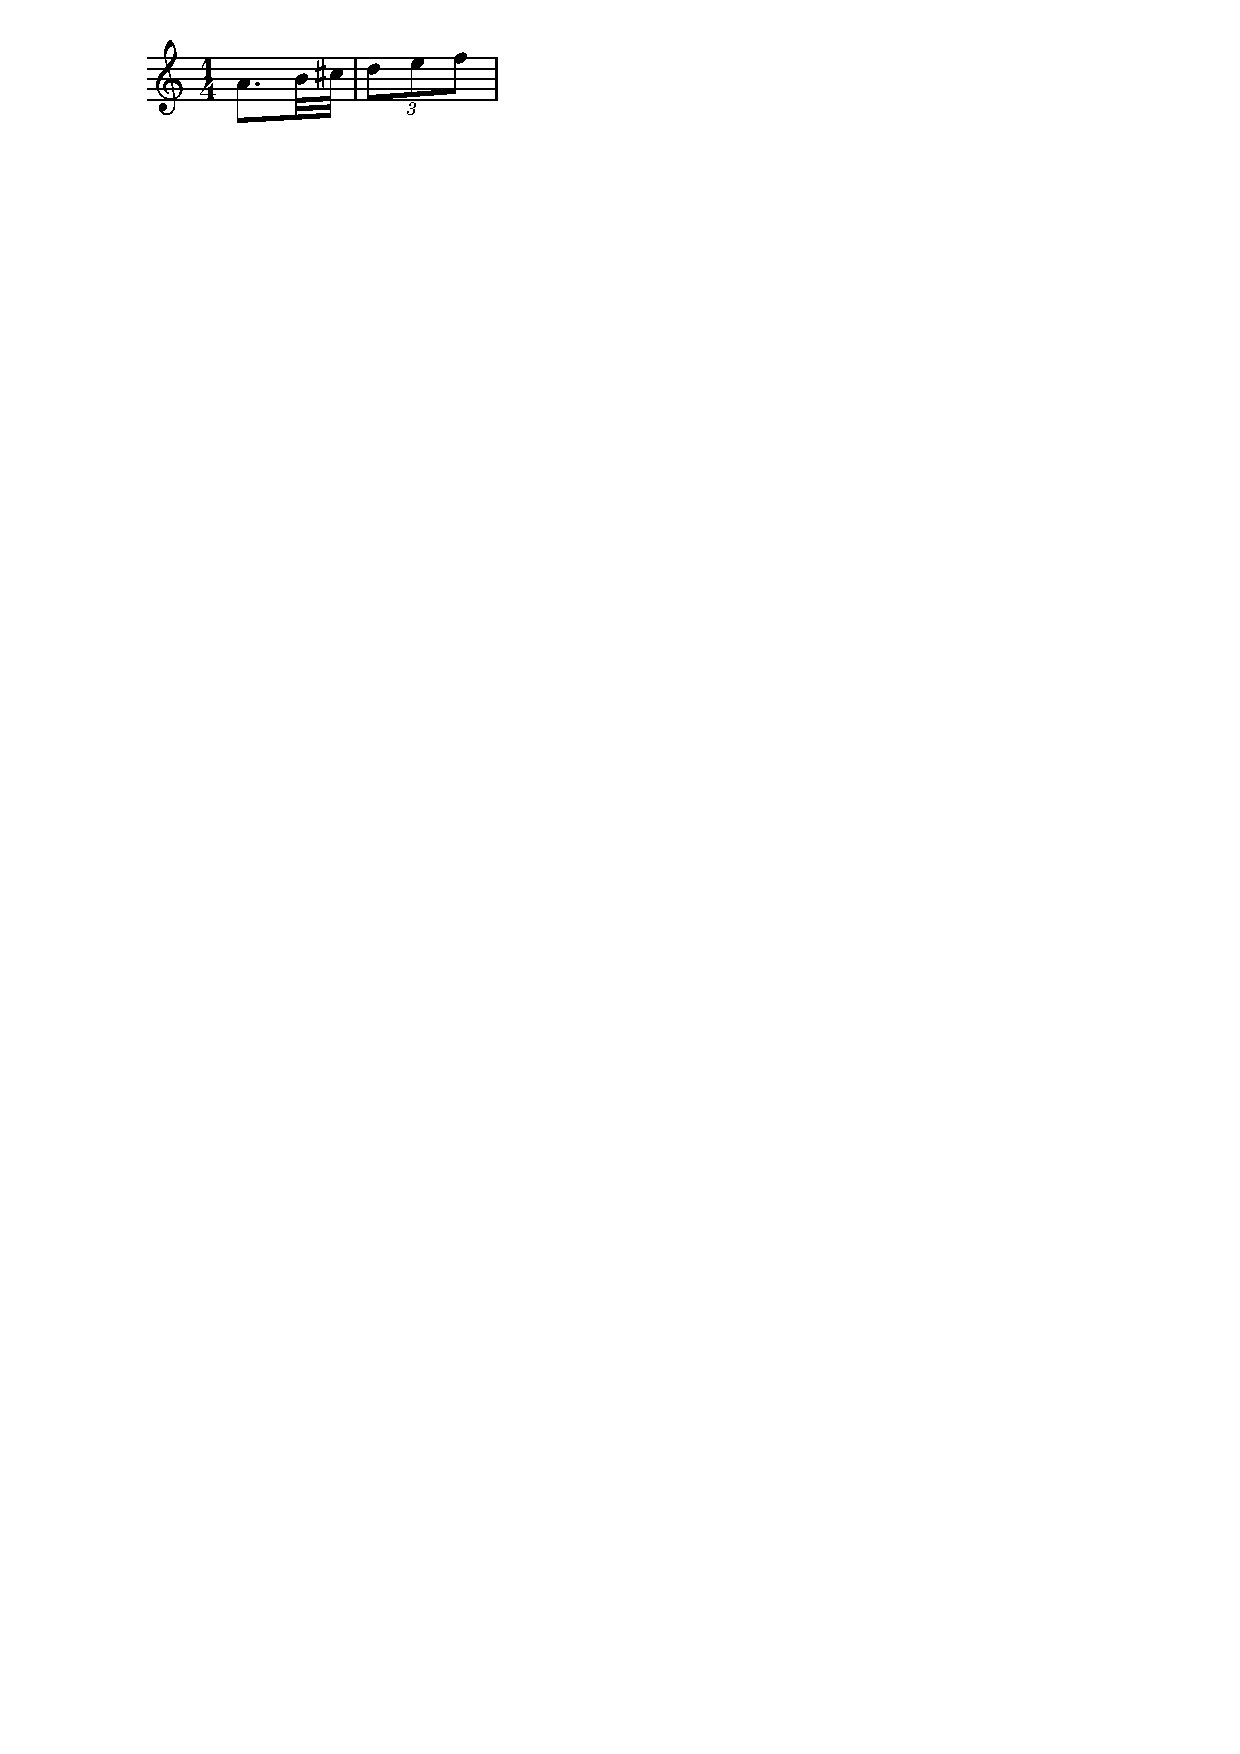
\includegraphics[scale=0.35,trim=0 5mm 0 0]{pictures/ex1.pdf},
%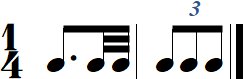
\includegraphics[scale=0.20]{pictures/score5.png}
will be favored on
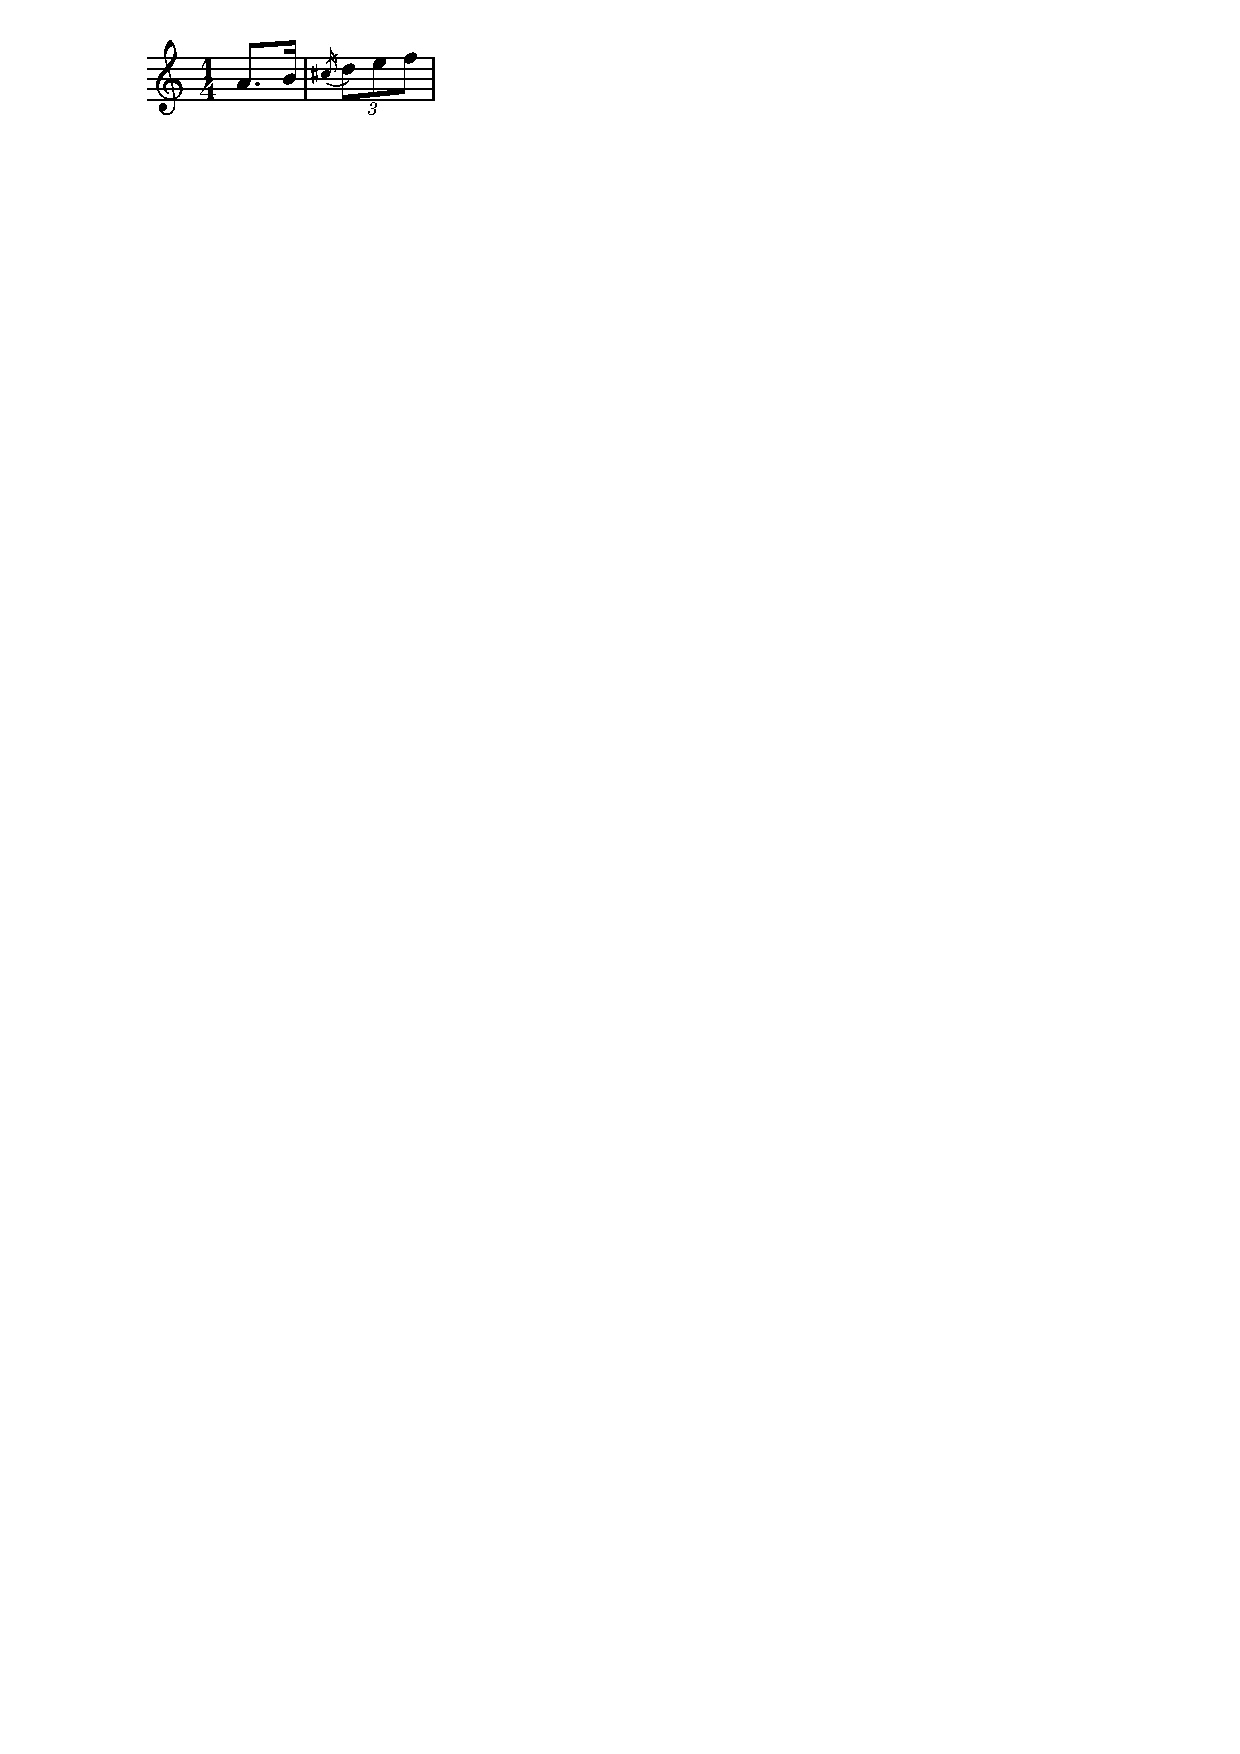
\includegraphics[scale=0.35,trim=0 5mm 0 0]{pictures/ex2.pdf}
%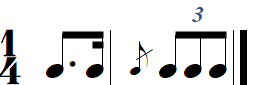
\includegraphics[scale=0.20]{pictures/score4.png}.
when the weight assigned to an additional second time division with $\ccall{2}$ is less
than the difference of weight between\
the appogiatura $\mbox{`\footnotesize C$\sharp$5`}$
and the standard note $\mbox{\footnotesize C$\sharp$5}$.

\noindent
The SW-parsing framework, applied to the transcription problem,
allows to find an optimal solution
that considers both the fitness of the result,
and its structural complexity.
\endex
\end{example}
The application to music transcription suggested briefly in the examples
has been implemented in a C++ tool~\cite{qparse}, %\footnote{https://qparse.gitlabpages.inria.fr}.
following the principles of the present SW-parsing framework, 
although it differs in several points.
In particular, the automata constructions are performed on the on-the-fly
during the search of a best AST, for efficiency reasons.


%
%\subsection{Computation}
%
\begin{proposition}
The problem of Symbolic Weighted Parsing
can be solved in PTIME in the size of the input \SWT $T$, \SWVPA $A$
and input word $s$,
and the computation time of the functions and operators of the label theory.
\end{proposition}
%
\begin{proof} (sketch)
We follow a \emph{Bar-Hillel} construction for parsing by intersection.
%
\noindent
We first extend the \SWT $T$ over $\Sigma$, $\Deltai$
into a \SWT $T'$ over $\Sigma$ and $\Delta$
(and the same semiring and label theory $\Semiring$ and $\bar\Phi$),
such that for every $u \in \Sigma^*$, and $t \in {\Delta}^*$,
$T'(u, t) = T(u, t|_{\Deltai})$.
%
$T'$ simply skips every symbol
$b \in {\Delta} \setminus \Deltai$
by the addition 
of new transitions of the form $\wei_{01}(q, \varepsilon, b, q')$ to $T$.
%
\noindent
Then, using Corollary~\ref{cor:epsilon},
we construct from $s \in \Sigma^*$ and $T'$
a \SWA $B_{s, T'}$,
such that for every $t \in \Delta^*$, $B_{s, T'}(t) = d(s, t)$.
%
%This automaton is such that for all $t \in \Delta^*$,
%\[
%   A_{T', s}\bigl(\lin(t)\bigr)
% = T'\bigl(s, \lin(t)\bigr)
% = T'\bigl(s, \lin(t)|_{\Deltai}\bigr)
% = d(s, t).
%\]
%
\noindent
Next, %we convert the input \SWTA $A$ over $\Delta$
%into a \SWVPA $A'$ over $\hat\Delta$, using Proposition~\ref{lem:SWTA}, and
we compute the \SWVPA $B_{s, T'} \otimes A$,
using Proposition~\ref{prop:SWVPA-product}.
%
\noindent
It remains to compute a best nested word $t \in {\Delta}^*$ for this \SWVPA,
using the procedure of Proposition~\ref{th:best-search}.
%and convert it into a best tree in $\T_\Delta$ in order to solve SW parsing
%for~$T$, $A$ and~$s$.
\qed
\end{proof}

The $\SW$-parsing problem generalizes
the problem of searching for the best derivation (AST) of a weighted CF-grammar $G$
that yields a given input word $w$, called~\emph{weighted parsing},
(see~\cite{Goodman99SemiringParsing},
 also the more general framework~\cite{MorbitzVogler19weighted-parsing}),
with an infinite input alphabet instead of a finite one and
transducer-defined distances instead of equality. 
%
See Appendix~\ref{sec:trees} for more details on the correspondence between 
nested words $t \in \Delta^*$, AST, CF grammars and \SWVPA.

%
%Indeed, it corresponds to the case where $T$
%accepts only the pairs $\<s, t>$ such that
%$s$ is the projection of $t$ on $\Deltai$.
%This can be done with a single state $q$ and
%with transition rules of the form:
%\begin{description}
%\item[] $\wei(q, \varepsilon, a, q) = \one$ for all $a \in \Deltac \cup \Deltar$,
%\item[] $\wei(q, a, a, q) = \one$ for all $a \in \Deltai$,
%\item[] $\wei(q, a, b, q) = \zero$ for all $a, b \in \Deltai$, $a \neq b$.
%\end{description}
%
%Weighted parsing
%corresponds to $\SW$-parsing in the case of finite alphabets,
%a transducer $T$ computing the identity and some \SWVPA~$A$
%obtained from $G$. %the weighted CF grammar.
%Indeed, the \emph{depth-first} traversal of an AST $\tau$
%yields a well-parenthesised word $\lin(\tau)$ over an alphabet
%$\Delta = \Deltai \uplus \Deltac \uplus \Deltar$,
%assuming \eg that $\Deltai$ contains the symbols labelling the leaves of $\tau$ 
%(symbols of rank $0$),
%and $\Deltac$ and $\Deltar$ contain respectively one left and right parenthesis
%$\ccall{b}$ and $\creturn{b}$ for each symbol $b$ labelling inner nodes of $\tau$ 
%(symbols of rank $>0$).
%
%With this representation, the projection $\lin(t)|_\Deltai$ is the
%sequence of leaves of $\tau$. %, enumerated in a \emph{dfs}-traversal.
%
%We show in Appendix~\ref{sec:trees} how to construct
%%($\SW$) tree automaton~$A$ %(in particular the TA computing on the AST of a given CF-grammar)
%a $\SWVPA$ $A$ such that $A(\lin(\tau))$ is the weight the AST $\tau$ of $G$.


%That also holds for the set of ASTs of a weighted CF-grammar.
%The purpose of the transducer $T$ is to measure a distance between input and output words,
%\ie between the word $s$ and the sequence leaves of a derivation tree, in $\Deltai^*$.
%
%that generates (weighted) trees by replacement of a state symbol~$q_0$ (non-terminal),
%by a tree $a(q_1,\ldots, q_k)$, where $k = \rank(a)$.
%A replacement rule $q_0 \to a(q_1,\ldots, q_k)$,
%of weight $\wei(q_0, a, q_1 \ldots q_k) \in \Semiring$
%according to Definition~\ref{def:SWTA},
%corresponds to the production rule $q_0 := a(q_1,\ldots, q_k)$ of a weighted CF grammar,
%with set non-terminal symbols $Q$ and set of terminal symbols $\Delta_0$.
%
%This actually is a slight generalization of CFG since
%each such production rule is labelled by  a symbol of $\Delta_{>0}$,
%hence parse trees %derivation trees
%are trees of $\T_\Delta)$.
%
%Another (more original) generalization is that the set of terminal symbols
%$\Delta_0$ may be infinite.
%
%
%The input language can also be expressed as a \SWTA, or,
%as a particular case, as a weighted context-free grammar,
%converted in turn into a \SWVPA following Lemma~\ref{lem:SWTA}.
%
%\florent{In practice,
%the functions in transition might be represented by diagram such as
%Algebraic Decision Diagrams~\cite{Bahar97ADD}.}
%\paragraph{Application to Automated Music Transcription.}
%



\subsection{Application to Automated Music Transcription}
\label{sec:transcription}
Symbolic Automated Music Transcription
and analysis of music performances

\subsubsection{Time Scales}
Real-Time Unit (RTU) = seconds

\noindent 
Musical-Time Unit (MTU) = number of measures

\noindent 
conversion via tempo value

\subsubsection{Representation of Music Performances}
We consider symbolic representations of musical performances, as finite sequences of events.
It corresponds to the concrete case of a MIDI file~\cite{SMF} 
recorded  from an electronic keyboard, 
or the output of a transcription from audio files~\cite{Benetos18AMTsurvey}.
%
For the sake of simplicity, 
we shall only consider here the case of monophonic performances, 
where at most one note is sounding at a time. 
The approach however extends to the polyphonic case.

A music performance is a finite sequence of events in a set~$\Sigma$.
Every event $e \in \Sigma$ has attributes such from a finite domain, 
like a number of key for a note 
or a flag indicating that it is a rest 
(\textsf{ON} and \textsf{OFF} messages in~\cite{SMF})
and a velocity value (0..127 in~\cite{SMF})).
%This representation is similar to the piano roll ~\cite{Muller15fundamentals} chap.1. 
Moreover, it contains a RTU value $\ioi{e}$ (real number) 
representing the time distance to the next event, 
or to the end of performance for the last event,
also called \emph{inter-onset interval}.


\subsubsection{Representation of Music Scores}
Music score are represented as structured words
made of timed %quantified 
events and parenthesized markups,
akin of nested words~\cite{AlurMadhusudan09nested}.

We consider an alphabet $\Delta$, every symbol of which is 
composed of a tag, in a finite set $\Xi$, 
and an MTU (rational) IOI duration value.
%The alphabet $\Delta$ 
It is partitioned into 
$\Delta = \Deltai \uplus \Deltac \uplus \Deltar$, 
like in Section~\ref{section:SWVPA}.
%
\noindent
The symbols of $\Deltai$ represent events:
% (infinite alphabet of internal symbols) made of:
with tags indicating a new note or grace-note (with null IOI), 
a rest or the continuation of the previous note (tie or dot).
%
The elements of $\Deltac \uplus \Deltar$ are matched
markups for describing the structure of the score, 
\ie the hierarchical grouping of events, and also, 
importantly the division of time in measures, tuplets...
%- parentheses for time divisions : tuplets, bars...
(linearization of rhythm trees \cite{jacquemard:hal-01138642}...).
They contain additional info such as tuple number, beaming policy...

\noindent
The duration values of letters of $\Delta$, in MTU (rational), 
can be computed with the markups and tags (\eg grace note has duration 0).

%\noindent
%There are simultaneous events, since grace notes has duration 0. They are ordered.
%
%\noindent
%Finite bound on the number of duration ratio. ?

\begin{example}
...      
\end{example}

\subsubsection{Performance/Score Distance Computation}
\label{app:distance}
We define a distance between performance and score representations
by a $\SWT$ $T = \< Q, \init, \wei, \final >$, over a semiring $\Semiring$.
** detail the elements of $\Semiring$ ....**
%are quadruplets of the form
%$\< t, s, \delta_t, \delta_s>$

Every state of $Q$ contains a 
tempo value in a finite domain (e.g. 30..300 bpm).
This value can be fixed 
or recomputed by the $T$ %transducer 
after reading each event, 
according to a perceptive/cognitive model of tempo 
such as~\cite{LargeJones99tempo}
(also used in the context of score following~\cite{Cont10TPAMI}).
% we wont detail here.


\subsection{Transcription by SW Parsing} %Best-first Search}
We assume a score language defined by a \SWVPA over the semiring 
$\Semiring$ of Section~\ref{app:distance}.


%...

\section*{Conclusion}

We  introduced Symbolic Weighted language models %over infinite alphabets,
and applied them to the problem of parsing
with infinitely many possible input symbols (typically timed events).
Our approach extends conventional parsing and weighted parsing
by computing a derivation tree modulo
a distance between words
defined by a SW transducer given in input.
This allows to consider finer word relationships than strict equality.
%

This work can be extended in several directions. First, 
the best search algorithm could be generalized from $1$-best to $n$-best~\cite{Huang05kbest},
and to $k$-\emph{closed} semirings~\cite{Mohri02semiring}
(instead of \emph{bounded}, which corresponds to $0$-\emph{closed}). Second,
%we believe that
the complexity bounds of the algorithms could be more precisely characterized,
as well as expressiveness of \swM compared to the automata of 
\eg~\cite{Segoufin06csl,KaminskiFrancez94,NevenSchwentickVianu04FSMinfinite,Bojanczyk11FO2}.
Finally, the  best search algorithm presented here works offline, whereas
an on-the-fly automata construction would allow for online parsing,
a suitable feature in the context of applications such as 
\eg automatic music transcription.

\florent{comparison of expressiveness with the automata 
of\cite{Segoufin06csl,KaminskiFrancez94,NevenSchwentickVianu04FSMinfinite,Bojanczyk11FO2}.}

\newpage


%%%%%%%%%%%%%%%%%%%%%%%%%%%%%%%%%%%%%%%%%%%%%%%%%%%%%%%%%%%%%%%%%%%%%%%%%%%%%%%%
%% BIBLIO                                                                     %%
%%%%%%%%%%%%%%%%%%%%%%%%%%%%%%%%%%%%%%%%%%%%%%%%%%%%%%%%%%%%%%%%%%%%%%%%%%%%%%%%
%\bibliographystyle{plain}
%\bibliographystyle{abbrv}
\bibliographystyle{plainurl}  % LIPICS
%\bibliographystyle{splncs04} % LLNCS
%\bibliographystyle{eptcs}    % EPTCS
%\bibliography{generic}

\bibliography{references}




%%%%%%%%%%%%%%%%%%%%%%%%%%%%%%%%%%%%%%%%%%%%%%%%%%%%%%%%%%%%%%%%%%%%%%%%%%%%%%%%
%% APPENDIX                                                                   %%
%%%%%%%%%%%%%%%%%%%%%%%%%%%%%%%%%%%%%%%%%%%%%%%%%%%%%%%%%%%%%%%%%%%%%%%%%%%%%%%%
\newpage
\appendix

%\section{Properties of Label Theory Operators} \label{sec:closure}
%% !TEX root = main.tex
%
% Properties of Label Theory

The following facts are immediate consequences of the definitions of 
the operators on the functions of labels theories. % in Section~\ref{sec:prelim}.

\begin{lemma} \label{lem:label-th}
For a complete label theory $\bar\Phi$, 
for all $\Phi_{\Sigma}, \Phi_{\Delta}, \Phi_{\Sigma, \Delta} \in \bar\Phi$, 
$\alpha \in \Semiring$,
$\phi, \phi' \in \Phi_{\Sigma}$,
$\psi \in \Phi_{\Delta}$, and
$\eta \in \Phi_{\Sigma, \Delta}$,
it holds that:
%
\begin{enumerate}
\item[$i.$]
\( \bigoplus_{\Sigma}\bigoplus^2_{\Delta} \eta = \bigoplus_{\Delta}\bigoplus^1_{\Sigma} \eta \).
\item[$ii.$]
\( \alpha \otimes \bigoplus_{\Sigma} \phi = \bigoplus_{\Sigma} (\alpha \otimes \phi) \) and
\( \bigl( \bigoplus_{\Sigma} \phi \bigr) \otimes\alpha = \bigoplus_{\Sigma} (\phi \otimes \alpha) \),
and similarly for~$\oplus$.
\item[$iii.$]
\( \bigl(\bigoplus_{\Sigma} \phi\bigr) \oplus \bigl(\bigoplus_{\Sigma} \phi'\bigr)
   = \bigoplus_{\Sigma} (\phi \oplus \phi') \) and
\( \bigl(\bigoplus_{\Sigma} \phi\bigr) \otimes \bigl(\bigoplus_{\Sigma} \phi'\bigr)
   = \bigoplus_{\Sigma} (\phi \otimes \phi') \).
\item[$iv.$]
\( \bigl(\bigoplus^2_{\Delta} \eta\bigr) \oplus \bigl(\bigoplus^2_{\Delta} \eta' \bigr) =
 \bigoplus^2_{\Delta} (\eta \oplus \eta') \), and
\( \bigl(\bigoplus^2_{\Delta} \eta\bigr) \otimes \bigl(\bigoplus^2_{\Delta} \eta' \bigr) =
 \bigoplus^2_{\Delta} (\eta \otimes \eta') \).
\item[$v.$]
%\( \phi \oplus \bigl(\bigoplus_{\Delta} \eta\bigr) = \bigoplus_{\Delta} (\phi \oplus \eta) \),
\( \phi \otimes \bigl(\bigoplus^2_{\Delta} \eta\bigr) = \bigoplus_{\Delta} (\phi \otimes_1 \eta) \), and
\( \bigl(\bigoplus^2_{\Delta} \eta\bigr) \otimes \phi = \bigoplus_{\Delta} (\eta \otimes_1 \phi) \),\\
and similarly for~$\oplus$.
\item[$vi.$]
%\( \psi \oplus \bigl(\bigoplus_{\Sigma} \eta\bigr) = \bigoplus_{\Sigma} (\psi \oplus \eta) \),
\( \psi \otimes \bigl(\bigoplus^1_{\Sigma} \eta\bigr) = \bigoplus_{\Sigma} (\psi \otimes_2 \eta) \), and
\( \bigl(\bigoplus^1_{\Sigma} \eta\bigr) \otimes \psi = \bigoplus_{\Sigma} (\eta \otimes_2 \psi) \),\\
and similarly for~$\oplus$.
\end{enumerate}
\end{lemma}


\section{End of proof of Proposition~\ref{prop:epsilon}} \label{sec:closure}
% !TEX root = main.tex
%
% Proof of Proposition closure swA by swT
%
Let us show that 
$B_{A, T}(t) = \displaystyle\bigoplus_{s\in \Sigma^*} A(s) \otimes T(s, t)$
for all $t\in \Delta^+$.

\noindent
We call \emph{run} from $\< p_0, q_0>$ to $\< p_n, q_n>$ 
a finite sequence of the form:
\florent{revise run with seq. of transitions}
$\rho = \< p_0, q_0>$, $a_1, \< p_1, q_1>$,\ldots, $a_n, \< p_n, q_n>$
where $\< p_i, q_i> \in Q'$ for all $0 \leq i \leq n$
and $a_j \in \Sigma$ for all $1 \leq j \leq n$.
The state $\< p_0, q_0>$ is called source of the run, denoted $\mathit{src}(\rho)$
and $\< p_n, q_n>$ is called target of the run, denoted $\mathit{trg}(\rho)$;
the set of runs with source $\< p, q>$ and target $\< p', q'>$ 
is denoted $\Rho(\< p, q>, \< p', q'>)$.
The word $a_1\ldots a_n \in \Sigma^*$ is called word of the run $\rho$
and denoted $\word(\rho)$.
%The set of all runs
Moreover, we associate a weight value in $\Semiring$ to every run, 
defined by:
\begin{equation} \label{def:weight-run}
\weight(\rho) = \bigotimes_{i = 1}^{n} 
\wei_1(p_{i-1}, a_i, p_i) \otimes
\wei_{10}(q_{i-1}, a_i, \varepsilon, q_i)
\end{equation}

By definition of the weight functions, and 
associativity, commutativity, and distributivity of $\oplus$, $\otimes$,  
it holds that:
\begin{equation}\label{eq:weight-run}
\weight_A(p, s, p') \otimes \weight_T(q, s, \varepsilon, q') = 
\bigoplus_{\begin{array}{c}
		   \scriptstyle\rho \in \Rho(\< p, q>, \< p', q'>)\\[-1ex]
		   %\scriptstyle\mathit{src}(\rho) = \<p , q>\\[-1ex]
		   %\scriptstyle\mathit{trg}(\rho) = \<p' , q'>\\[-1ex]
		   \scriptstyle\word(\rho) = s
		   \end{array}} 
\weight(\rho) 
\end{equation}
%
Using \eqref{def:weight-run} 
and Lemma~\ref{lem:label-th} repetively, 
\eqref{eq:weight-run} implies that:
%
\begin{equation}\label{eq:weight-run-plus}
\begin{array}{l}
\displaystyle\bigoplus_{s \in \Sigma^*} 
  \weight_A(p, s, p') \otimes \weight_T(q, s, \varepsilon, q') =\\
\multicolumn{1}{r}{%
\qquad
\displaystyle\bigoplus_{\begin{array}{c}
		   \scriptstyle\rho \in \Rho(\< p, q>, \< p', q'>)\\[-1ex]
		   \scriptstyle\rho = \< p_0, q_0>, a_1,\< p_1, q_1>,\ldots, a_n, \< p_n, q_n>\\[-1ex]
%		   \scriptstyle\rho = \< p_0, q_0>, a_1,\\[-1ex]
%		   \scriptstyle\< p_1, q_1>,\ldots,\\[-1ex]
%       	   \scriptstyle a_n, \< p_n, q_n>\\[-1ex]
%		   \scriptstyle\< p_0, q_0> = \< p, q>\\[-1ex]
%		   \scriptstyle\< p_n, q_n>  = \< p', q'>	   
		   \end{array}} 
\displaystyle\bigotimes_{i = 1}^{n} 
\displaystyle\bigoplus_\Sigma (\wei_1(p_{i-1}, p_i) \otimes
                  \wei_{10}(q_{i-1}, q_i))
}
\end{array}           %\nonumber
\end{equation}
%
Note that the symbols $a_1, \ldots, a_n \in \Sigma$ in the run $\rho$
are not significant in \eqref{eq:weight-run-plus}.
%
Using a pumping argument, we can show that~\eqref{eq:weight-run-plus}
still holds when restricting $\rho$ to the set $\Rho_0(\< p, q>, \< p', q'>)$
of runs without repetition in the state symbols.
%
Indeed, assume that in 
$\rho = \< p_0, q_0>, a_1,\< p_1, q_1>,\ldots, a_n, \< p_n, q_n>$, 
$\< p_{i_1}, q_{i_1}> = \< p_{i_2}, q_{i_2}>$
for $0 \leq i_1 < i_2 \leq n$.
Then 
$\rho' = 
 \< p_0, q_0>, \ldots, 
 a_{i_1-1},\< p_{i_1-1}, q_{i_1-1}>,
 a_{i_2},\< p_{i_2}, q_{i_2}>, \ldots,  a_n, \< p_n, q_n>$ 
also belongs to   $\Rho\bigl(\< p_0, q_0>, \< p_n, q_n>\bigr)$
and yields a smaller expression (\wrt $\leq_\oplus$) 
in the right-hand-side of \eqref{eq:weight-run-plus}
than~$\rho$.
It follows, by~\eqref{eq:init-wei} and \eqref{eq:iter-wei}, that
for all $b \in \Delta$, 
%
\begin{equation}\label{eq:weiprime1}
%\begin{array}{rcl}
\wei'_1(\< p, q>, b, \< p', q'>) = 
\displaystyle\bigoplus_{s \in \Sigma^*} 
\displaystyle\bigoplus_{\begin{array}{c}
                        \scriptstyle p'' \in P\\[-1ex]
                        \scriptstyle q'' \in Q
                        \end{array}}
\weight_A(p, s, p'') \otimes \weight_T(q, s, \varepsilon, q'') \otimes \psi_1(b)
%\weight_{B_{A, T}}(\< p, q>, s, \< p', q'>)
%\end{array}
\end{equation}
where 
$\psi_1 = \wei_{01}(q'', q') \oplus
\displaystyle{\bigoplus}_\Sigma^1 \bigl(\wei_1(p'', p') 
 \otimes_1 \wei_{11}(q'', q')\bigr)$.
%
% lift to $A(s) \otimes T(s, \varepsilon)$

\medskip
\noindent
We show now by induction on the length of $t \in \Delta^+$, that
\[
\weight_{B_{A, T}}(\<p, q>, t, \<p', q'>) = 
 \displaystyle\bigoplus_{s\in \Sigma^*}
 \weight_{A}(p, s, p') \otimes  \weight_{T}(q, s, t, q')
\]
This permits to conclude, using 
the definition of $\init'$ in~\eqref{eq:initprime},
%and a proof for 
and the definition of $\final'$ 
in~\eqref{eq:init-final}, and~\eqref{eq:iter-final}. 
%$B_{A, T}(t) = \displaystyle\bigoplus_{s\in \Sigma^*} A(s) \otimes T(s, t)$

\noindent
The base case $t \in \Delta$ follows from~\eqref{eq:weiprime1} and 
the distributivity of $\otimes$.

\noindent
For $t = b u$, with $b \in \Delta$ and $u \in \Delta^*$,
by definition of $\weight_A$ and $\weight_T$,
it holds that for all $s \in \Sigma^*$:
\[
\begin{array}{l}
\displaystyle\weight_A(p, s, p') \otimes \weight_T(q, s, t, q') = 
\bigoplus_{s = s_1 s_2}
\displaystyle\bigoplus_{\begin{array}{c}
                        \scriptstyle p'', p''' \in P\\[-1ex]
                        \scriptstyle q'', q''' \in Q
                        \end{array}}
\weight_A(p, s_1, p''') \otimes \weight_A(p''', s_2, p'') \mathop\otimes \\
\hfill\displaystyle
\weight_T(q, s_1, \varepsilon, q'') \otimes
 \left(
 \begin{array}{l}
 \displaystyle
 \bigoplus_{q''' \in Q}
 \wei_{01}(q'', \varepsilon, b, q''') \otimes \weight_T(q''', s_2, u, q')
 \mathop\oplus\\
 \displaystyle
 \bigoplus_{q''' \in Q} \bigoplus_{s_2 = a s'_2}
 \wei_{11}(q'', a, b, q''') \otimes \weight_T(q''', s'_2, u, q')
 \end{array}
 \right)
\end{array}
\]

\noindent
Using~\eqref{eq:weiprime1}, it follows that:
\[
\begin{array}{l}
\displaystyle\bigoplus_{s \in \Sigma^*} 
\displaystyle\weight_A(p, s, p') \otimes \weight_T(q, s, t, q') = \\
\qquad
\displaystyle\bigoplus_{\begin{array}{c}
                        \scriptstyle p'', p''' \in P\\[-1ex]
                        \scriptstyle q'', q''' \in Q
                        \end{array}}
\bigoplus_{s_1 \in \Sigma^*}
\weight_A(p, s_1, p'') \otimes \weight_T(q, s_1, \varepsilon, q'') \otimes \psi_1(b)\\
%\wei'_1(\< p, q>, b, \< p'', q''>) \mathop\otimes \\
\qquad
\otimes\displaystyle\bigoplus_{\scriptstyle s_2 \in \Sigma^*}
\weight_A(p''', s_2, p') \otimes \weight_T(q''', s_2, u, q')
%\displaystyle\bigoplus_{\begin{array}{c}
%                        \scriptstyle s_1 \in \Sigma^*\\[-1ex]
%                        \scriptstyle s_2 \in \Sigma^*
%                        \end{array}}
\end{array}
\]
with 
$\psi_1 = \wei_{01}(q'', q''') \oplus
\displaystyle{\bigoplus}_\Sigma^1 \bigl(\wei_1(p'', p''') 
 \otimes_1 \wei_{11}(q'', q''')\bigr)$.

\noindent
The first term in the right-hand-side is 
$\wei'_1(\< p, q>, b, \< p''', q'''>)$ by \eqref{eq:weiprime1},
and the second term is
$\weight_{B_{A,T}}(\< p''', q'''>, u, \< p', q'>)$ by induction hypothesis.
Hence, by definition, 
\[
\begin{array}{rcl}
\displaystyle\bigoplus_{s \in \Sigma^*} 
\displaystyle\weight_A(p, s, p') \otimes \weight_T(q, s, t, q') & = & \\
\multicolumn{3}{r}{%
\displaystyle\bigoplus_{\begin{array}{c}
                        \scriptstyle p''' \in P\\[-1ex]
                        \scriptstyle q''' \in Q
                        \end{array}}
 \wei'_1(\< p, q>, b, \< p''', q'''>) \otimes
 \weight_{B_{A,T}}(\< p''', q'''>, u, \< p', q'>)}\\
 & = & \weight_{B_{A,T}}(\< p, q>, t, \< p', q'>).\\
\end{array}
\]




%
%
% old version
%
%\noindent
%The entering, leaving and transition functions of $B_{A, T}$ will
%simulate synchronized computations of $A$ and $T$,
%while reading an output word of $\Delta^*$.
%%
%Its state entering functions is defined
%for all $\<p_1, q_1> \in Q'$, %$p_1 \in P$, $q_1 \in Q$
%by $\init'(p_1, q_1) = \init_A(p_1) \otimes \init_T(q_1)$.
%%
%The transition function $\wei'_1$ will roughly perform
%a synchronized product of transitions defined by $\wei_1$,
%$\wei_{01}$ ($T$ reading in output word and not an input word)
%and $\wei_{11}$ ($T$ reading both an input word and an output word).
%%
%Moreover, $\wei'_1$ also needs to simulate transitions
%defined by $\wei_{10}$: $T$ reading in input word and not an output word.
%Since $B_{A, T}$  will read only in the output word, such a transition corresponds
%to an $\varepsilon$-transition of $\SWA$.
%But $\SWA$ have been defined without $\varepsilon$-transitions.
%Therefore, in order to take care of this case, we perform an on-the-fly
%suppression of $\varepsilon$-transition in the $\SWA$ in construction,
%following the algorithm of~\cite{LombardySakarovitch12ciaa}.
%%
%% Initialize state leaving functions i
%%and $\final'(p, q) = \final_A(p) \otimes \final_T(q)$.
%
%%Every transition of $B_{A, T}$ will
%%simulate a sequence of transitions of $T$ performing the following steps:
%%advance in the input word while staying immobile in the output word,
%%and then make one step in the output word (and advance in the input word or not).
%
%\noindent
%Initially, for all $p_1, p_2 \in P$, and $q_1, q_2 \in Q$, let
%\[
%\begin{array}{rcl}
%\wei'_1\bigl( \< p_1, q_1>, \< p_2, q_2>\bigr) & = &
%\wei_1(p_1, p_2) \otimes
%\bigl[
%\wei_{01}(q_1, q_2)
%\oplus
%\displaystyle\bigoplus_{\Sigma}
%\wei_{11}(q_1, q_2)
%\bigr]\\
%\final'(p_1, q_1) & = & \final_A(p_1) \otimes \final_T(q_1)
%\end{array}
%\]
%
%\noindent
%Then, we iterate the following for all $p_1\in P$ and $q_1, q_2 \in Q$:
%for all $p_2\in P$ and $q_3 \in Q$,
%\[
%\begin{array}{rcl}
%\wei'_1\bigl( \< p_1, q_1>, \< p_2, q_3>\bigr) & \opluseq &
%\displaystyle\bigoplus_{\Sigma} \wei_{10}(q_1, q_2)
%\otimes
%\wei'_1\bigl( \< p_1, q_2>, \< p_2, q_3>\bigr)\\
%\final'(p_1, q_1) & \opluseq &
%\displaystyle\bigoplus_{\Sigma} \wei_{10}(q_1, q_2)
%\otimes \final'(p_1, q_2)
%\end{array}
%\]

%\section{Proof of Proposition~\ref{prop:SWVPA-product}} \label{sec:product}
%% !TEX root = main.tex
%
% Proof of Proposition product swVPA
%
We prove the closure under $\otimes$. 
The proof of the closure under $\oplus$ is similar.

Let $A_1 = \< Q_1, P_1, \init_1, \bar\wei_1, \final_1 >$
and $A_2 = \< Q_2, P_2, \init_2, \bar\wei_2, \final_2 >$.
The \SWVPA $A_1 \otimes A_2$ is built by a 
classical product construction.
%
It has a state set $Q = Q_1 \times Q_2$
and a auxiliary set of stack symbols $P = P_1 \times P_2$:
$A_1 \otimes A_2 = \< Q, P, \init_{1, \otimes}, 
         \bar\wei_{\otimes}, \final_{\otimes} >$.
The weight entering and leaving functions         
$\init_{\otimes}$, $\final_{\otimes}$
and the sextuplet of transition functions $\bar\wei_{\otimes}$
are defined 
using the label-theory operators of Section~\ref{section:symbols}.
They will simulate the synchronized behaviour of $A_1$ and $A_2$.
%
For all $\< q_1, q_2>, \< q'_1, q'_2> \in Q$ 
and $\< p_1, p_2>, \< p'_1, p'_2> \in P$:
\[
\begin{array}{lcl}
\init_{\otimes}\bigl(\< q_1, q_2>\bigr) & = & \init_{1}(q_1) \otimes \init_{2}(q_2)\\
\final_{\otimes}\bigl(\< q_1, q_2>\bigr) & = & \final_{1}(q_1) \otimes \final_{2}(q_2)\\
%
\wei_{\mathsf{i}, \otimes}\bigl(\< q_1, q_2>, \<p_1, p_2>, \<q'_1, q'_2>\bigr) & = &
\wei_{\mathsf{i}, 1}(q_1, p_1, q'_1) \otimes \wei_{\mathsf{i}, 2}(q_2, p_2, q'_2)\\
%
\weie[\mathsf{i}, \otimes]\bigl(\< q_1, q_2>, \<q'_1, q'_2>\bigr) & = &
\weie[\mathsf{i}, 1](q_1, q'_1) \otimes \weie[\mathsf{i}, 2](q_2, q'_2)\\
%
\wei_{\mathsf{c}, \otimes}\bigl(\< q_1, q_2>, \<p_1, p_2>, \<q'_1, q'_2>, \<p'_1, p'_2>\bigr) & = &
\wei_{\mathsf{c}, 1}(q_1, p_1, q'_1, p'_1) \otimes \wei_{\mathsf{c}, 2}(q_2, p_2, q'_2, p'_2)\\
%
\weie[\mathsf{c}, \otimes]\bigl(\< q_1, q_2>, \<p_1, p_2>, \<q'_1, q'_2>\bigr) & = &
\weie[\mathsf{c}, 1](q_1, p_1, q'_1) \otimes \weie[\mathsf{i}, 2](q_2, p_2, q'_2)\\
%
\wei_{\mathsf{r}, \otimes}\bigl(\< q_1, q_2>, \<p_1, p_2>, \<q'_1, q'_2>\bigr) & = &
\wei_{\mathsf{r}, 1}(q_1, p_1, q'_1) \otimes \wei_{\mathsf{r}, 2}(q_2, p_2, q'_2)\\
%
\weie[\mathsf{r}, \otimes]\bigl(\< q_1, q_2>, \<q'_1, q'_2>\bigr) & = &
\weie[\mathsf{r}, 1](q_1, q'_1) \otimes \weie[\mathsf{i}, 2](q_2, q'_2)\\
\end{array}
\]








%\section{Correctness of the Best-Search Algorithm} \label{sec:bestsearch}
%% !TEX root = main.tex
%
% Proof of best-search algo


The correctness of Algorithm~\ref{algo:Dijkstra}
is stated by the following lemma.

\begin{lemma}\label{lem:bot}
At the termination of Algorithm~\ref{algo:Dijkstra}, 
for all $\< q_1, q_2> \notin \Q$,
$d_\bot(q_1, q_2) =  b_\bot(q_1, q_2)$.
\end{lemma}

The proof is by contradiction,
assuming a counter-example minimal in the length of the witness word.

is ensured by the invariant... expressed in the following lemma.

\begin{lemma}\label{lem:top}
At every step of Algorithm~\ref{algo:Dijkstra}, 
for all $\< q_1, p, q_2> \notin \Q$,
$d_\top(q_1, p, q_2) = b_\top(q_1, p, q_2)$.
\end{lemma}

\noindent
For computing the minimal weight of a computation of $A$, we use the equality~\eqref{eq:min}, 
which, with Lemma~\ref{lem:bot} implies that
at the termination of Algorithm~\ref{algo:Dijkstra}, %it holds that,
%There exist $q_1, q_2 \in Q$
\(
  {\displaystyle \bigoplus_{s \in \Delta^*} A(s)} =
  {\displaystyle\bigoplus_{q, q' \in Q}} \textstyle
  \mathsf{in}(q) \mathop{\otimes} d_\bot(q, q') \mathop{\otimes} \mathsf{out}(q').
\)

\section{Nested Words and Parse Trees} \label{sec:trees}\label{app:trees}
% !TEX root = main.tex
%
% Correspondance between nested-words and trees

The hierarchical structure of nested words, defined with the \emph{call} 
and \emph{return} markup symbols
suggest a correspondence with trees.
The lifting of this correspondence to languages, of tree automata and VPA,
has been discussed in~\cite{AlurMadhusudan09nested},
and~\cite{Caralp12VPAmult} for the weighted case.
In this section, we describe a correspondence between the symbolic-weighted extensions
of tree automata and VPA.

Let $\Omega$ be a countable ranked alphabet, such that
every symbol $a \in \Omega$ has a rank
$\rank(a) \in [0..M]$ where $M$ is a fixed natural number.
We denote by $\Omega_k$ the subset of all symbols $a$ of $\Omega$
with $\rank(a) = k$, where $0 \leq k \leq M$,
and $\Omega_{>0} = \Omega \setminus \Omega_0$.
%
\noindent
The free $\Omega$-algebra of finite, ordered,
$\Omega$-labeled trees is denoted by $\T_\Omega$.
It is the smallest set such that  $\Omega_0 \subset \T_\Omega$
and for all $1 \leq k \leq M$, all $a \in \Omega_k$,
and all $t_1, \ldots, t_k \in \T_\Omega$, $a(t_1, \ldots, t_k) \in \T_\Omega$.
%
% tree = single node (leave) labeled with a symbol of $a \in \Omegai$
% (such a tree is simply denoted by $a$)
% or the composition, denoted by $b(t_1,\ldots, t_n$) of a node labeled with $b$
% and $n$ subtrees $t_1$,\ldots, $t_n$.
%
Let us assume a commutative semiring~$\Semiring$
and a label theory~$\bar{\Phi}$ over~$\Semiring$
containing one set~$\Phi_{\Omega_k}$ for each $k \in [0..M]$.
%
\renewcommand{\call}[1]{\ensuremath \langle_{#1}}
\renewcommand{\return}[1]{\ensuremath {}_{#1}{\rangle}} % $\prescript{}{a}{)}$

% A \emph{regular tree grammar} over $\Omega$
% is a triplet $G = \< N, q_\mathsf{i}, R>$ where
% $N$ is a finite set of non-terminal symbols denoted $q$...,
% $q_\mathsf{i} \in N$ is the starting non-terminal,
% $R$ is a finite set of production rules of the form
% $q_0 \to a(q_1\ldots q_k)$ where
% $q_0, q_1, \ldots, q_k \in N$
% $a \in \Omega_k$.
% A tree $t \in \T_\Omega$ is in the language of $G$
% if it can be generated from $q_\mathsf{i}$ by
% non terminal replacement following the rules of $R$.
%
\begin{definition}  \label{def:SWTA}
A \emph{symbolic-weighted tree automaton} (\SWTA)
over $\Omega$, $\Semiring$, and~$\bar\Phi$
is a triplet $A = \< Q, \init, \bar{\wei} >$ where
$Q$ is a finite set of states,
$\mathsf{in} : Q \to \Phi_\Omega$ is the starting weight function,
and $\bar{\wei}$ is a tuplet of transition functions containing,
for each $k \in [0..M]$,
%$\wei_\varepsilon$ from $Q \times Q$ into $\Semiring$, and,
the functions $\wei_{k}: Q \times Q^{k} \to \Phi_{\Omega_{>0},\Omega_k}$
and $\weie[k]: Q \times Q^{k} \to \Phi_{\Omega_k}$.
\end{definition}
%
%Like in Section~\ref{sec:SWAdef},
We define %from $\bar{\wei}$
a transition
function~$\wei: Q \times (\Omega_{> 0} \cup \{ \varepsilon \}) \times \Omega \times \bigcup_{k=0}^{M} Q^k
  \to \Semiring$
by: %also called $\wei$ for simplicity,
%such that, for all $q, q' \in Q$, $a \in \Sigma$, and $b \in \Delta$,
\[
\begin{array}{rcll}
%\wei(q_0, \varepsilon, q_1) & = &  \wei_\varepsilon(q_0, q_1),\\ %\phi_\varepsilon\\
\wei(q_0, a, b, q_1 \ldots q_k) & = & \eta(a, b) &
\quad\mathrm{where~} \eta = \wei_{k}(q_0, q_1\ldots q_k)\\
\wei(q_0, \varepsilon, b, q_1 \ldots q_k) & = & \phi(b) &
\quad\mathrm{where~} \phi = \weie[k](q_0, q_1\ldots q_k).
\end{array}
\]
%
\noindent
where $q_1\ldots q_k$ is $\varepsilon$ if $k = 0$.
The first case deals with a strict subtree, with a parent node labeled by $a$,
and the second case is for a root tree.

\noindent
Every \SWTA %of Definition~\ref{def:SWTA}
defines a mapping
from trees of $\T_\Omega$ into~$\Semiring$, %the weight values in~$\Semiring$,
based on the following intermediate function
$\weight_A: Q \times (\Omega \cup \{ \varepsilon \}) \times \T_\Omega \to \Semiring$
\begin{equation}
%\begin{array}{rccl}
\weight_A(q_0, a, t) =  % & = &
%   \displaystyle\bigoplus_{q_1 \in Q} &
%   \wei(q, \varepsilon, q_1) \otimes \weight_A(q_1, t)\\
 \displaystyle\bigoplus_{q_1 \ldots q_k \in Q^k} % &
              \wei(q_0, a, b, q_1 \ldots q_k )
   \otimes \displaystyle\bigotimes_{i=1}^{k}
           \weight_A(q_i, b, t_i)
%\end{array}
\end{equation}
where $q_0 \in Q$, $a \in \Omega_{>0} \cup \{ \varepsilon \}$ and
$t = b(t_1,\ldots, t_k) \in \T_\Omega$,
$0 \leq k \leq M$.

\medskip\noindent
Finally, the weight associated by $A$ to  $t \in \T_\Omega$ is
\begin{equation}
A(t)  =
\displaystyle\bigoplus_{q \in Q} \mathsf{in}(q) \mathop{\otimes} \weight_A(q, \varepsilon, t)
\label{eq:weightTA}
\end{equation}

\noindent
Intuitively, $\wei(q_0, a, b, q_1 \ldots q_k)$ can be seen as
the weight of a production rule $q_0 \to b(q_1, \ldots, q_k)$
of a regular tree grammar~\cite{tata},
that replaces the non-terminal symbol $q_0$ by $b(q_1, \ldots, q_k)$,
provided that the parent of $q_0$ is labeled by $a$
(or $q_0$ is the root node if $a = \varepsilon$).
%in a step of tree building.
%
%Such a grammar computes the weights of the derivation trees
%of the Context-Free grammar obtained by forgetting the labeling symbols of $\Omega_{>0}$.
The above production rule can also be seen as
a rule of a weighted CF grammar, of the form
$[a, b]\, q_0 := q_1 \ldots q_k$ if $k > 0$,
and $[a]\, q_0 := b$ if $k = 0$.
In the first case, $b$ is a label of the rule,
and in the second case, it is a terminal symbol.
And in both cases, $a$ is a constraint on the label of rule applied
on the parent node in the derivation tree.
This features of observing the parent's label
are useful in the case of infinite alphabet,
where it is not possible to memorize a label with the states.
%
%One can observe that
\noindent The weight of a labeled derivation tree $t$
of the weighted CF grammar associated to~$A$ as above,
is $\weight_A(q, t)$,
when $q$ is the start non-terminal.
%
We shall now establish a correspondence between such a derivation tree $t$
and some word describing a linearization of $t$,
in a way that $\weight_A(q, t)$ can be computed by a $\SWVPA$.

Let $\hat\Omega$ be the countable (unranked) alphabet obtained
from $\Omega$ by:
$\hat\Omega = \Deltai \uplus \Deltac \uplus \Deltar$, with
$\Deltai = \Omega_0$,
$\Deltac = \{ \; \call{a} \mid a \in \Omega_{>0} \}$,
$\Deltar = \{ \; \return{a} \mid a \in \Omega_{>0} \}$.

\noindent
We associate to $\hat\Omega$
a label theory $\hat{\Phi}$
like in Section~\ref{sec:SWVPA-def},
%
\noindent
and we define a linearization of trees of $\T_\Omega$ into
words of ${\hat\Omega}^*$ as follows:
\begin{description}
\item $\lin(a) = a$ for all $a \in \Omega_0$,
\item $\lin\bigl( b(t_1, \ldots, t_k)\bigr) =
       \call{b} \; \lin(t_1) \ldots \lin(t_k) \; \return{b}$
       when $b \in \Omega_k$ for $1 \leq k \leq M$.
\end{description}
%
\begin{example}
The trees in Figure~\ref{fig:score-tree}
represent the two scores in Examples~\ref{ex:running},\ref{ex:nested-word}, 
and their linearization are respectively~$O$ and~$O'$ inn the same examples.
\end{example}


\begin{proposition}\label{lem:SWTA}
For all \SWTA $A$ over~$\Omega$, $\Semiring$ commutative, and $\bar\Phi$,
there exists an effectively constructible \SWVPA $A'$ over
$\hat\Omega$, $\Semiring$ and $\hat\Phi$
such that for all $t \in \T_\Omega$, $A'\bigl(\lin(t)\bigr) = A(t)$.
\end{proposition}
%
\begin{proof}
Let $A = \< Q, \init, \bar{\wei} >$ where $\bar{\wei}$ is presented as above by a function
    %
We build
$A' = \< Q', P', \init', \bar{\wei}', \final' >$,
%computing over $\Delta = \Omegai \uplus \Omegac \uplus \Omegar$,
where $Q' = \bigcup_{k=0}^{M} Q^k$ is the set of sequences of state symbols of $A$,
of length at most $M$, including the empty sequence denoted by~$\varepsilon$,
and where $P' = Q'$ and $\bar\wei$ is defined by:

\[
\begin{array}{lcll}
\weii(q_0\, \bar{u}, {\call{c}}, \bar{p}, a, \bar{u}) & = & \wei(q_0, c, a, \varepsilon) &
\mathrm{for~all~} c \in \Omega_{>0}, a \in \Omega_0\\ %\bar{p}\in P',
%
\weiei(q_0\,\bar{u}, a, \bar{u}) & = & \wei(q_0, \varepsilon, a, \varepsilon) &
\mathrm{for~all~} a \in \Omega_0\\
%
\weic(q_0\,\bar{u}, {\call{c}}, \bar{p}, \call{d}, \bar{u}, \bar{q}) & = & \wei(q_0, c, d, \bar{q}) &
\mathrm{for~all~} c, d \in \Omega_{>0}\\ % \bar{p}\in P'
%
\weiec(q_0\,\bar{u}, \call{c}, \bar{u}, \bar{q}) & = & \wei(q_0, \varepsilon, c, \bar{q}) &
\mathrm{for~all~} c \in \Omega_{>0}\\
%
%\weir: Q \times \Omegac \times P \times \Sigmar \times Q \to \Semiring &
\weir(\varepsilon, {\call{c}}, \bar{p}, {\return{c}}, \bar{p}) & = & \one &
\mathrm{for~all~}  c \in \Omega_{>0}\\ % \bar{p}\in P'
%
%\weie: Q \times \Omegar \times Q \to \Semiring &
\weier(\bar{u}, {\return{c}}, \bar{q}) & = & \zero &
\mathrm{for~all~}  c \in \Omega_{>0}
\end{array}
\]
\noindent
All cases not matched by one of the above equations have a weight $\zero$,
for instance  %This is in particular the case of
$\weir(\bar{u}, {\call{c}}, \bar{p}, {\return{d}}, \bar{q}) = \zero$
if $c \neq d$
or $\bar{u} \neq \varepsilon$
or $\bar{q} \neq \bar{p}$.
%
%\noindent
%It is sufficient to consider in $Q'$ only the prefixes of
%sequences in transition with a non-null weight.
%\qed
\end{proof}

\begin{figure}
\begin{center}
\begin{tikzpicture} [-,thick]
\tikzstyle{level 1}=[level distance=9mm,sibling distance=24mm]
\tikzstyle{level 2}=[level distance=8mm,sibling distance=6mm]
\tikzstyle{level 3}=[level distance=8mm,sibling distance=6mm]
\node {$\mathsf{m}$}
  child { node {$2$}
    child { node {$\mbox{\footnotesize A4}$} }
    child { node {$2$}
      child { node {$-$} }
      child { node {$2$}
        child { node {$\mbox{\footnotesize B4}$} }
        child { node {$\mbox{\footnotesize C$\sharp$5}$} }}}}
  child { node {$\mathsf{m}$}
    child { node {$3$}
      child { node {$\mbox{\footnotesize D5}$} }
      child { node {$\mbox{\footnotesize E5}$} }
      child { node {$\mbox{\footnotesize F5}$} }}
    child { node {$\varepsilon$} }};        
\end{tikzpicture}
%
\quad 
%
\begin{tikzpicture} [-,thick]
\tikzstyle{level 1}=[level distance=9mm,sibling distance=30mm]
\tikzstyle{level 2}=[level distance=8mm,sibling distance=8mm]
\tikzstyle{level 3}=[level distance=8mm,sibling distance=8mm]
\node {$\mathsf{m}$}
  child { node {$2$}
    child { node {$\mbox{\footnotesize A4}$} }
    child { node {$2$}
      child { node {$-$} }
      child { node {$\mbox{\footnotesize B4}$} } } }
  child { node {$\mathsf{m}$}
    child { node {$3$}
      child { node {$`\mbox{\footnotesize C$\sharp$5}`\,\mbox{\footnotesize D5}$} }
%                   {$\begin{array}{c}
%                     \mbox{\footnotesize C5}\\
%                     \mbox{\footnotesize D5}
%                     \end{array}$} }
      child { node {$\mbox{\footnotesize E5}$} }
      child { node {$\mbox{\footnotesize F5}$} } }
    child { node {$\varepsilon$} } };        
\end{tikzpicture}
\end{center}
\caption{Tree representation of scores 
of Examples~\ref{ex:running},\ref{ex:nested-word}, 
linearized respectively into~$O$ and~$O'$.}
\label{fig:score-tree}
\end{figure}




%%%%%%%%%%%%%%%%%%%%%%%%%%%%%%%%%%%%%%%%%%%%%%%%%%%%%%%%%%%%%%%%%%%%%%%%%%%%%%%%
%% TODO                                                                       %%
%%%%%%%%%%%%%%%%%%%%%%%%%%%%%%%%%%%%%%%%%%%%%%%%%%%%%%%%%%%%%%%%%%%%%%%%%%%%%%%%
%\newpage
%\listoftodos


\end{document}
